\documentclass[12pt]{article}
\usepackage[english]{babel}
\usepackage{amsmath,amsfonts}
\usepackage{amsthm}
\usepackage{amssymb}
\usepackage{amscd}
\usepackage{fancyhdr}
\usepackage{graphicx}
\usepackage{setspace}
\usepackage{verbatim}
\usepackage{tikz-cd}
\usepackage{pdfsync}
\usepackage{stmaryrd}
\usepackage{calrsfs}
\usepackage{mathrsfs}
%\usepackage{hyperref}
\usepackage[a4paper,left=1cm,right=1cm,top=3cm,bottom=1.5cm]{geometry}
\usetikzlibrary{positioning, arrows}
%\usepackage[a4paper,left=2cm,right=2cm,top=2cm,bottom=3.5cm]{geometry}
\pdfpagewidth 12in
\pdfpageheight 15in

\pagestyle{fancy}
\fancyhf{}
%\renewcommand{\headrulewidth}{0pt}
\headheight 15pt
\rhead{\rightmark}
\lhead{Graduate Algbera II-A script}
\rfoot{}
\cfoot{\thepage}
\lfoot{}
\title{}
\author{}

\theoremstyle{definition}
\newtheorem{Rmk}{Remark}[section]
\newtheorem{Ex}{Example}[section]
\newtheorem{apDef}{Definition}
\newtheorem{Def}{Definition}[section]
\newtheorem{Lemma}{Lemma}[section]
\newtheorem{Cor}{Corollary}[section]
\newtheorem{Exe}{Example}[section]
\newtheorem{Prop}{Proposition}[section]
\newtheorem{Theo}{Theorem}[section]
\newtheorem*{noRmk}{Remark}

\theoremstyle{plain}

%%%%%%%%%%%%%%%%%%%%%%%%%%%%%%%%%%%%%%%%%%%%5
\DeclareMathOperator*{\Span}{Span}
\DeclareMathOperator{\tr}{tr}
\DeclareMathOperator{\sign}{sgn}
\DeclareMathOperator{\id}{id}
\DeclareMathOperator{\im}{Im}
\DeclareMathOperator{\inv}{Inv}
\DeclareMathOperator{\codim}{codim}
\DeclareMathOperator{\ind}{ind}
\DeclareMathOperator{\defect}{def}
\DeclareMathOperator{\Spec}{Spec}
\DeclareMathOperator{\nil}{nil}
\DeclareMathOperator{\rad}{rad}
\DeclareMathOperator{\Hom}{Hom}
\DeclareMathOperator{\End}{End}
\DeclareMathOperator{\Coker}{Coker}
\DeclareMathOperator{\CoIm}{CoIm}
\DeclareMathOperator{\rank}{rank}
\DeclareMathOperator{\Ann}{Ann}
\DeclareMathOperator{\ev}{ev}
\DeclareMathOperator{\Ext}{Ext}
\DeclareMathOperator{\Tor}{Tor}
\DeclareMathOperator{\Adj}{Adj}
\DeclareMathOperator{\Aut}{Aut}
\DeclareMathOperator{\Ht}{ht}
\DeclareMathOperator{\supp}{supp}
\DeclareMathOperator{\gr}{gr}
%%%%%%%%%%%%%%%%%%%%%%%%%%%%%%%%%%%%%%%%%%%%%%%%%%%%%%%%%%%%
\newcommand{\tabs}[1]{\interleave #1 \interleave}
\newcommand{\lbrac}[1]{\left\{ #1 \right\}}
\newcommand*{\bigchi}{\mbox{\Large$\chi$}}% big chi
%%%%%%%%%%%%%%%%%%%%%%%
\newcommand{\quat}{\mathbb{H}}
\newcommand{\nat}{\mathbb{N}}
\newcommand{\real}{\mathbb{R}}
\newcommand{\complex}{\mathbb{C}}
\newcommand{\rat}{\mathbb{Q}}
\newcommand{\z}{\mathbb{Z}}
\newcommand{\field}{\mathbb{F}}
\newcommand{\inj}{\hookrightarrow}
\newcommand{\surj}{\twoheadrightarrow}
%%%%%%%%%%%%%for this document%%%%%%%%%%%%%%%%%%%%%%
\newcommand{\sn}{\Delta^n}
\newcommand{\smoo}{C^\infty}
\newcommand{\vecf}{\mathfrak{X}(M)}
\newcommand{\overbar}[1]{\mkern 1.5mu\overline{\mkern-1.5mu#1\mkern-1.5mu}\mkern 1.5mu}
\newcommand{\brac}[1]{\langle #1 \rangle}
\renewcommand{\bar}{\overbar}
\renewcommand{\tilde}{\widetilde}
\newcommand{\disk}{\mathbb{D}}
\newcommand{\torus}{\mathbb{T}}

%\hypersetup{colorlinks=true, linkcolor=red, pdfborderstyle={/S/U/W 1}}
\begin{document}
\tableofcontents
\pagebreak
\section{Introduction}
  Reference Text:
  \begin{enumerate}
    \item Michael Atiyah, \emph{Introduction to commutative algebra}.
    \item Matsumura, \emph{Commutative Ring theory}, Cambridge series.
    \item Jean Serre, \emph{Local Algebra}, Springer.
  \end{enumerate}
  $\nat={0,1,....}$
\subsection{Rings and algebras}
The reader is assumed to be familiar with the fundamentals of rings.
\Exe[examples of rings from number theory]\leavevmode
\begin{enumerate}
  \item \textbf{Gaussian integer} $\z[i]$
  \item \textbf{Eisenstein integer} $\z[\omega]$ where $\omega=\frac{-1+\sqrt{3}i}{2}$ the root of $x^2+x^2+1$. (Note: $\omega^2=-1-\omega$)
  \item polynomial algebras over a coefficient ring $A$:
  $$A[x]:=\{\text{formal sums } \sum_{i\in \nat^n}a_ix^i\}$$
  where the coefficients are almost all zero. (Note the $i$ is multi-index, and $x^i=x_1^{i_1}...x_n^{i_n}$). The identity $\id_{A[x]}=1\cdot x$.
  \item Rings of functions on geometric objects: $C(X, \real)$, $C^\infty(X, \complex)$ etc.
\end{enumerate}
\Exe [p-adic no.]
\begin{equation}
\begin{tikzcd}
  & \z \arrow[hook]{ld} \arrow[hook]{r}\arrow[hook]{d} & \rat \arrow[hook]{d} \arrow[hook]{r} &\real \arrow[hook]{r}&\complex
  \\ \field_p &\z_p\arrow[hook]{l} \arrow[hook]{r} &\rat_p & &
\end{tikzcd}
\end{equation}
\Prop [Universal Property of the zero ring] For any ring $A$, there exists a unique ring homomorphism form $A$ to $0$.
\Rmk Geometrically for any set $X$, $\exists !$ set map $\varphi: \phi\to X$
\Prop [Universal Property of the ring $\z$] For any ring $A$< $\exists !$ ring homomorphism: $\z\to A$
\proof $f:\z\to A$: $n\geq 0: f(n)=n\cdot 1_A$; $n<0, f(n)=-f(-n)$.
\Rmk Geometrically for any set $X$, $\exists !$ set map $\varphi: X\to \{\cdot\}$.
\Def Let $A$ be a commutative ring. An $A$-algebra (commutative algebra) consists of:\leavevmode
\begin{enumerate}
  \item A ring $B$ (underlying ring of the $A$-algebra)
  \item a ring $\varphi_B:A\to B$ (structural homomorphism of $B$ as $A$-algebra)
\end{enumerate}
\Rmk In context of $A$-algebras, anything in $A$ is considered `known'.
\Exe Any commutative ring is canonically and uniquely a $\z$-algebra, immediately from the universal property of $\z$.
\Exe Given base ring $A$, the polynomial algebra $A[x]$ is an $A$-algebra. with structural homomorphism $A\to A[x]: a\mapsto ax^{(0,...,0)}$.
\Prop [Universal property of $A$-algebra] For any $A$-algebra $B$, and any $n$ elements $b_1,..., b_n\in B$: $\exists ! A$-algebra homomorphism: $f:A[x_1, ..., x_n]\to B$ such that $f(x_1)=b_1, ..., f(x_n)=b_n$.
\Def If $B, C$ are $A$-algebra, an $A$-algebra homomorphism: $B\to C$ is a map such that $f$ is a ring homomorphism and the diagram commutes:
\begin{equation}\begin{tikzcd}
B \arrow{rr}{f}
& &C\\
&A\arrow{lu}{\varphi_B} \arrow{ru}[swap]{\varphi_C}
\end{tikzcd}
\end{equation}
$f\circ \varphi_B=\varphi_C$.
\Def Let $A$ be base ring. Let $B$ be a $A$-algebra. A \textbf{sub-$A$-algebra} of $B$ (a.k.a., \textbf{subring} of $B$ when $A=\z$) is a additive subgroup which is closed under multiplication of $B$ and contains $1_B$. Moreover, the structural homomorphism $\varphi_B: A\to B$ maps into $C$. i.e. $\varphi_B: A\overset{\varphi_C}{\to} C \hookrightarrow B$.
\Rmk When we speak of subring, the last prerequisite becomes unnecessary.
\Exe $\complex[X^2, Y^3]\subseteq \complex[X, Y]$
\Def Let $A$ be a base ring. $\{B_i\}_{i\in I}$ be a family of $A$-algebra. The direct product $A$-algebra of the family is a $A$-algebra given by underlying ring: $\prod_{i\in I}B_i$ with conventional zero and identity. and the $A$-algebra structural homomorphism given by $$\varphi_{\prod B_i}:A\to \prod_{i\in I}B_i; \qquad a\mapsto (\varphi_{i}(a))_{i\in I}$$
\Rmk The direct product comes with projection maps. $\forall j\in I$, we have $$\pi_j:\prod B_i\to B_j; \qquad (b_i)_{i\in I}\mapsto b_j$$.
\Prop[Universal property of direct product] Given any $A$-algebra $C$ and $\forall j\in I$, given an $A$-algebra homomorphism $f_j:C\to B_j$, $\exists ! A$-algebra homomorphism $f: C\to \prod B_i$  such that $\forall j\in I$, the diagram commutes.
\begin{equation}\begin{tikzcd}
\prod B_i\ar[two heads]{r}{\pi_j} &B_j\\
C\arrow{u}{f_i} \ar[dashed]{ru}[swap]{\tilde{f}}
\end{tikzcd}
\end{equation}
\Def A \textbf{subring} of a ring $A$ is a subset $B\subseteq A$ such that $B$ is an additive subgroup and is closed under multiplication which contains $1_A$. An \textbf{ideal} of a ring $A$ is a subset $I\subseteq A$ such that $I$ is an additive subgroup which $\forall a\in A, \forall x\in I, ax\in I$.
\Def Given a ring $A$ and an ideal $I\subseteq A$, a \textbf{quotient ring of $A$ modulo $I$} is the ring $A/I$ with the canonical map:
$$\pi: A\to A/I; a\mapsto a+I$$
which is a surjective ring homomorphism.
\Exe $A/\{0_A\}\cong A \qquad A/A\cong 0 \qquad \z/n\z$ the ring of integers modulo $n$.
\Prop [Universal Property of quotient ring] Given a ring $A$ and an ideal $I$. Then for any ring and a ring homomorphism $f:A\to B$, such that for all $a\in I$, $f(x)=0$. Then it induces an unique ring homomorphism $\tilde{f}:A/I\to B$ making the following diagram commutes.
\begin{equation}\begin{tikzcd}
A\ar{r}{f} \ar[two heads]{d}[swap]{q}&B\\
C\arrow[dashed]{ru}[swap]{\tilde{f}}
\end{tikzcd}
\end{equation}
\Rmk $f^{-1}(\text{any ideal of }B$ is an ideal of $A$. Hence when $q:A\twoheadrightarrow A/I$ the quotient homomorphism. Then there is a bijection:
\begin{align*}
  \{\text{radicals of }A\supseteq I\} &\longleftrightarrow \{\text{ideals of }A/I\}\\
  J(\supseteq I)&\to q(J)=J/I
\end{align*}
More precisely, we have the following isomorphism theorem:
\Theo For any homomorphism $f:A\to B$, there induces an isomorphism of rings: $\tilde{f}:A/\ker(f)\cong \im(f)$. In addition, the following diagrams commutes:
\begin{equation}
  \begin{tikzcd}
    A\ar{r}{f} \ar[two heads]{d}{q} & B\\
    A/\ker(f) \ar{r}{\tilde{f}}[swap]{\cong} & f(A)\ar[hook]{u}
  \end{tikzcd}
\end{equation}
\Def Given $A$ a ring. Then $x\in A$ is a \textbf{zero-divisor} if $\exists y\in A\backslash\{0\}$, such that $x\cdot y=0_A$. $x\in A$ is \textbf{nilpotent element} if $\exists \in \nat$ such that $x^n=0_A$. $x\in A$ is \textbf{invertible} if $\exists y\in A$ such that $x\cdot y=1_A$.
\Exe In $\z/6\z$, then $2+6\z$ and $3+6\z$ are zero divisors which does not have nilpotent element.
\Def We define a ring $A$ to be a \textbf{integral domain}(or for brevity \textbf{domain}) if $A\neq 0$ and $A$ does not possess any zero-divisors other than zero. We say a ring $A$ is \textbf{reduced} if $A$ does not possess any nilpotent elements other than zero.

\bigskip
\subsection{prime and maximal ideals}
\Def An ideal $\mathfrak{p}\subsetneq A$ is a \textbf{prime ideal} of $\forall a, b\in A$ such that $a\cdot b\in \mathfrak{p}$ then either $a\in \mathfrak{p}$ or $b\in \mathfrak{p}$.
\Rmk When $\mathfrak{p}$ is prime, then $A/\mathfrak{p}$ is a integral domain.
\Def An ideal $\mathfrak{m}\in A$ is \textbf{maximal} if $\mathfrak{m}\neq A$ and is maximal with respect to inclusion. i.e., $\forall I\supsetneq \mathfrak{m}$, $I=A$.
\Rmk $\mathfrak{m}$ is maximal $\iff$ $A/\mathfrak{m}$ is a field.
\Rmk Given a family of ideals $\{I_j=i\}$ of $A$. Then the intersection $\bigcap_{i\in I}I_i\subseteq A$ is an ideal, so is the sum $\sum_{i\in I}I_i$, where $\sum_{i\in I}I_i$ is the intersection of all ideals containing $I_j$, i.e., the \textbf{ideal generated by $\{I_i\}$}.
\Prop Let $f:A\to B$ a ring homomorphism. Then for any prime ideal $\mathfrak{q}\in B$, $f^{-1}(\mathfrak{q}\in A)$ is also a prime ideal.
\proof Consider the following diagram:
\begin{equation}
  \begin{tikzcd}
    A\ar{r}{f} \ar[two heads]{d} \ar[two heads]{rrd}{g}&B \ar[two heads]{r}{\pi} &B/\mathfrak{q}\\
    A/f^{-1}(\mathfrak{q})\ar{rr}{\cong} & &g(A)\ar[hook]{u}[swap]{\id}
  \end{tikzcd}
\end{equation}
where $A/f^{-1}(\mathfrak{q})$ is either $0$ or $A$. But $f^{-1}(\mathfrak{q})\neq A$, for $a\notin f^{-1}(\mathfrak{q})$. Hence $A/f^{-1}(\mathfrak{q})$ is a integral domain.
\Prop [Existence of maximal ideals for non-zero rings] Let $A$ be a non-zero ring. then $\exists$ a maximal (hence prime) ideal in $A$.
\proof Zorn's Lemma and note the set of proper ideals of $A$ is not empty, containing zero ideal.
\Cor Let $A$ be a non-zero ring. $\mathfrak{a}\subsetneq A$ be a proper ideal. Then $\exists $ a maximal ideal $\mathfrak{m}\subseteq A$ such that $\mathfrak{a}\subseteq \mathfrak{m}$.
\proof Apply the proposition to $A/\mathfrak{a}$.
\Cor Let $A$ be a non-zero ring. $a\in A\backslash A^\times$ be any non-invertible element. Then $\exists$ maximal ideal containing $a$.
\Def Let $I\subseteq A$ be ideal. The \textbf{radical of $I$} is
$$\rad(I):=\{a\in A: \exists n\in \nat, a^n\in I\}$$
The \textbf{nilradical of $A$} is
$$\nil(A):=\rad(\text{zero ideal in }A)=\{a\in A:\exists n\in \nat, a^n=0_A\}$$
\Rmk $\rad(I)\supseteq I$ an ideal. If $a, b\in \rad(I)$, so is $a+b$.
\Prop $\nil(A)=\bigcap$ all prime ideals in $A$.
\proof $\subseteq$ is clear. For the direction of $\supseteq$, suppose $a$ is not nilpotent. Consider $A[1/a]:=A[X]/(aX-1)$. we show this ring is nonzero. Assuming this, choose a maximal hence prime ideal $\mathfrak{q}\subseteq a[1/a]$and the ring homomorphism:\begin{align}
  A\hookrightarrow A[x]&\twoheadrightarrow A[1/a]\\
  f^{-1}\mathfrak{q}=\mathfrak{p} &\mapsto \mathfrak{q}
\end{align}
hence $a\notin \mathfrak{p}$. \\
Now we show $A[1/a]\notin 0$. Suppose $A[1/a]=0$. then $A[1/a]\iff (aX-1)\cdot A[X]=A[X]\iff \exists \varphi(X):=a_0+a_1X+...+a_nX^n\in A[X]$ such that $(aX-1)\cdot \varphi(X)=1\in A[X]$. Then $a_0=1, a\cdot a_0=a$, $a_2=a\cdot a_1=a^2$... $a_r=a\cdot a_{n-1}=a^n$ and $a\cdot a_n=0$. Hence $a$ is nilpotent.
\Rmk The spirit of this proof is to construct a new ring in which the original elements becomes invertible. So is this the method of localisation.

\bigskip
\subsection{Zariski topology}
\Def Let $A$ be a ring. Then the \textbf{prime spectrum of ring $A$} is
$$\Spec{A}:=\{\text{prime ideals of }A\}$$
 For any subset $E\subseteq A$, we define:
\begin{align*}
  V(E)&:=\{\mathfrak{p}\in \Spec(A): \mathfrak{p}\subseteq E\}\\
  &=\{\text{all prime ideals of }A\subseteq E\}
\end{align*}
So $V(E)\subseteq \Spec(A)$.
\Def We define the \textbf{Zariski topology} on $\Spec(A)$ being defining the closed sets in $\Spec(A)$ to be:
$$\mathcal{C}:=\{\text{collection of all these }V(E): E\in A\}$$
\Rmk One could readily verifies the axioms of topology fulfilled with the following Lemmas. The others are left to the reader.
\Lemma \begin{gather}
  V(E)=V(\text{ideals in }A\text{ generated by }E)\\
  \bigcap_{i\in I}V(E_i)=V(\bigcup_{i\in I}E_i) \qquad \bigcap_{i\in I}V(a_i)=V(\sum_{i\in I}a_i)\\
  \text{for any ideals }\mathfrak{a}, \mathfrak{b}\subseteq A, V(\mathfrak{a}\cap \mathfrak{b})=V(\mathfrak{a}\mathfrak{b})=V(\mathfrak{a})\cap V(\mathfrak{b})
\end{gather}
where $\mathfrak{a}\mathfrak{b}$ denotes the product ideals.
\proof $\mathfrak{p}$ prime ideal of $A$ contains $E$ $\iff$ it contains an ideal generated by $E$. If $\mathfrak{p}\supseteq \mathfrak{a}\cap \mathfrak{b}\supseteq \mathfrak{a}\mathfrak{b}$, hence $\mathfrak{p}\supset\mathfrak{a}$ or $\mathfrak{p}\supseteq\mathfrak{b}$.
\Ex \leavevmode
\begin{enumerate}
  \item $\Spec(\field)$={zero ideals of $\field$} is a singleton.
  \item $\Spec(\z)$={zero ideal $0\z$} $\cap$ {$p\z$: $p$ prime number}, where closed sets are $V(a\z: a\in \z)=\{p \text{ prime }: p|a\}$, which is a finite union of $V(p\z)=\{p\z\}$. Moreover, except of $\Spec(\z)$ itself, no closed subset contains $0\z$
\begin{noRmk}
 To express the topology on $\z$ explicitly, we have $(0)$ be not closed point, and $(p)$ are all closed points. Yet $\bar{\{0\z\}}$ is $\Spec(\z)$. Hence $\{0_\z\}$ is dense in $\Spec(\z)$, testifying that Zariski topology are in general not Hausdorff. This may sometimes, however, be a virtue. We we exploit an set $X$, which possess an certain desired property. Showing $X$ is closed and $0\z\in X$ shall be sufficient to extend $X$ to all prime ideals of $\z$, that is, $\Spec(\z)$.
 \end{noRmk}
  \item $\Spec(\field[x])$=\{Zero ideals $0\cdot \field[x]$\}$\cap$ \{$f\cdot \field[x]$: $f$ monic polynomials irreducible over $\field$\}, where the closed sets are finite union of $\{f\cdot \field[x]\}$  where $f$ monic polynomials irreducible over $\field$.
 \begin{noRmk}[\textbf{Special case $\field=\complex$}]\leavevmode
   \begin{align*}
    \Spec(\complex[x])&\cong \{0\}\sqcup \complex/\{\alpha\sim (x-\alpha):\alpha\in \complex\} \\
     \Spec(\real[x])&\cong \{0\}\sqcup \real/\{\alpha\sim(x-\alpha):\alpha\in\real\}\sqcup\{\text{orbits of }(\complex\backslash\real)\text{ under complex conjugation}\}\\
     &\cong \quat/\{\alpha\sim((x-\alpha)(x-\bar{\alpha}))\}
   \end{align*}
 \end{noRmk}
\end{enumerate}
\Prop Let $f:A\to B$ be a ring homomorphism. Define
\begin{align}
  f^*: \Spec(B)&\to \Spec(A)\\
  \mathfrak{q}& \mapsto f^*(\mathfrak{q}):=f^{-1}\mathfrak{q}:=\{a\in A: f(a)\in \mathfrak{q}\}
\end{align}
Then this map is well defined by the results of last time. Then $f^*$ is continuous in Zariski topology.
\proof It is equivalent to show that $\forall$ closed set $C$ in $\Spec(A)$ $(f^*)^{-1}(C):=\{y\in \Spec(y); y\in C\}$ closed. Set $X:=\Spec(A), Y:=\Spec(B)$, then $f^*:Y\to X$, Let $C\subseteq X$ closed, then $\exists \mathfrak{a}\subseteq A$ such that $C=V_A(\mathfrak{a})$. Let $\mathfrak{b}:=$ ideal of $B$ generated by $f(\mathfrak{a})$. Let $D:=V_Y(\mathfrak{b})$ closed in $Y$. We claim $(f^*)^{-1}(C)=D$. \\ Let $\mathfrak{q}\subseteq B$ be a prime ideal. then
\begin{align*}
  \mathfrak{q}\in (f^*)^{-1}(C) &\iff (f^*)(\mathfrak{q})\in C\\
   &\iff f^{-1}(\mathfrak{q})\supseteq \mathfrak{a} \text{ as ideals in } A\\
    &\iff f(\mathfrak{a})\subseteq \mathfrak{q}\\
    &\iff \mathfrak{b}\subseteq \mathfrak{q}\text{ as ideal in }B\\
    &\iff q\in V_Y(\mathfrak{b})=D
\end{align*}
\Prop If $f:A\to B$, and $g:B\to C$ are ring homomorphisms. Then $(g\cdot f)^*=f^*\cdot g^*$ with $1^*$ the identity on $\Spec$.
\Def for $f\in A$, Define $X_f=X\backslash V(f)=\{\mathfrak{p}\in \Spec(A):f\notin\mathfrak{p}\}$ is called a \textbf{principal/basic open subset} of $\Spec(A)$.
\Lemma Any open subset $U\in \Spec(A)$ and any $x\in U$, $\exists$ principal open $X_f\in X$ such that $x\in X_f\subseteq U$.
\proof Given $x\in U=X\backslash V(\mathfrak{a})$ for some $\mathfrak{a}\in A$, where $x$ corresponds to a prime ideal $\mathfrak{p}\subseteq A$ such that $\mathfrak{p}\not\supseteq \mathfrak{a}$. Hence $\exists f\in \mathfrak{a}\backslash \mathfrak{p}$, Hence we yield $X_f$ principal open, where since $f\in \mathfrak{a}$, hence $X_f\subseteq A\backslash V(\mathfrak{a})=U$, also since $f\notin \mathfrak{p}$, $\mathfrak{p}$ belongs to $X_f$.
\Rmk Following the lemma, $X_{\text{invertible element}}=X_1=X; X_{\text{nilpotent element}}=\emptyset; X_f\cap X_g=X_{fg}$.
\Prop $\Spec(A)=X$ is \textbf{quasi-compact} if $X$ assumes a finite-subcovering for every covering.
\Rmk According to French \textbf{AND} German school, \bf{compact=quasi-compact+hausdorff}.
\proof Let $\{U_i\}_{i\in \mathfrak{I}}$ be a covering of $x$. So $X=\bigcap_{i\in \mathfrak{I}}U_i$. Because $X_f$ form bases of Zariski-topology, hence we may assume $U_i=X_{f_i}$ for some $f_i$ is principal open. So $X=\bigcup_{i\in \mathfrak{I}}X_{f_i}$, equivalent to say every prime ideals avoid some $f_i$. Hence let $I:=$ ideal in $A$ generated by all $f_i$, hence $I\subsetneq A$ an ideal hence must contain $1$, hence $\exists$ finitely many $i_1,..., i_n\in I$ and with $g_j\in A$ such that $1=f_1g_1+...+f_ng_n\in A$. It follows that no prime ideal $\mathfrak{p}\in A$ contains all $f_1, ..., f_n$. Hence $X=X_{f_1}\cup...\cup X_{f_n}$.

\bigskip
\subsection{Modules}
\Def A \textbf{module over a ring $A$} consists:
\begin{itemize}
  \item an abelian group $M$ (underlying additive group)
  \item a map $A\times M\to M$ (scalar multiplication map) \\ \medskip satisfying: $\forall a, b\in A$, $m, m'\in M$,
  \item $(ab)\cdot m=a(b\cdot m)$
  \item $1_A\cdot m=m$
  \item $(a+b)\cdot m=a\cdot m+b\cdot m$
  \item $a\cdot (m+m')=a\cdot m+a\cdot m'$
\end{itemize}
\Rmk Equivalently, an $A$-module consists of an additive group $M$ and a ring homomorphism $\varphi_M:A\to \End(M)$ and define scalar multiplication $a\cdot m=\varphi_M(a)(m)$.
\Exe \leavevmode
\begin{itemize}
  \item When $A$ is a field, $A$-module is $A$-vector space.
  \item When $A=\z$, $A$-module is an abelian group.
  \item Zero $A$-module $0$ consisting $\{0\}$.
  \item \textbf{Regular $A$-module} when $M=A$ as a canonically $A$-module.
  \item If $\varphi:A\to B$ is a ring homomorphism, then $B$ becomes an $A$-module via $\varphi$.
\end{itemize}
\Def Let $M, N$ be a $A$-module. An $A$-module homomorphism from $M$ to $N$ consists of a map $f:M\to N$ compatible with the addition of underlying group and respects the scalar multiplication in $M$.
\Prop [Universal property of zero module] For any $A$-module $M$, $\exists !$ $A$-module homomorphism $M\to 0$  and $\exists ! $ $A$-module homomorphism $0\to M$.
\Rmk So $0$ are both the initial and final objects in the category of $A$-module.
\Prop [Universal property of $A$-module $A$] For any $A$-module $M$ and any $m\in M$, $\exists !$ $A$-module homomorphism $f:A\to M$ such that $f(1_A)=m$.
\Def Let $M, N$ be $A$-module. Then the \textbf{Hom-modules} $\Hom_A(M, N)$ is the $A$-module with pointwise addition and pointwise scalar multiplication.
\Rmk let $M, N, P$ be $A$-module. Then $\Hom_A(N, P)\times \Hom_A(M, N)\to$ $\Hom_A(M, P)$ is $A$-bilinear.
\Def Let $\{M_i\}_{i\in I}$ be a family of $A$-module. their \textbf{direct product} is the $A$-module:
\begin{align*}
  \prod_{i\in I}M_i&:=\{\text{all set theoretic maps }m:I\to \sqcap_{i\in I}M_i: \forall i\in I, m(i)\in M_i\}
  \\ &=\{\text{co-tuples}(m_{i_1}, ...) \text{ indexed by }i\in I: m_i\in M_i\}
\end{align*}
where the scalar multiplication obvious.Their \textbf{direct sum} is the $A$-module:
\begin{align*}
  \bigoplus_{i\in I}M_i:=\{(m_i)_{i\in I}\in \prod_{i\in I}M_i: m_i \text{ are all but finitely many non-zero}\}
\end{align*}
\Prop [Universal Property of $\prod$] For any $A$-module $M$ and any family of $A$-module homomorphism, $\{f_j:M\to M_j\}_{j\in I}$ such that $\exists !A$-module homomorphism $f:M\to \prod_{i\in I}M_i$ such that the following diagram commutes:
\begin{equation}\begin{tikzcd}
\prod M\ar[dashed]{r}{f} \ar{rd}[swap]{f_j}&\prod_{i\in I}M_i\ar{d}[two heads]{\pi_j}\\
& M_j
\end{tikzcd}
\end{equation}
\Prop [Universal Property of $\bigoplus$] For any $A$-module $M$ and any family $A$-module homomorphism $\{g_i: M_j\in M\}$, $\exists ! A$-module $g:\bigoplus_{i\in I}M_i\to M$ such that the following diagram commutes:
\begin{equation}\begin{tikzcd}
\bigoplus_{i\in I}M_i\ar[dashed]{r}{g} &B_j\\
C\arrow{u}{\iota_i} \ar{ru}[swap]{g_j}
\end{tikzcd}
\end{equation}
\Def An \textbf{$A$-submodule} is a subset of $A$ which is closed under $+, 0, -$ and also closed under scalar multiplication of $M$.
\Exe $0, M$ are both submodules of $M$. If $\{N_j\}$ is a family of sub-$A$-modules of $M$, then $\cap N_j$ and $\sum_{j]in J}N_j$ are also submodules of $M$. Moreover, as we had in rings, if $f:M\to N$ an $A$-module homomorphism, then the image of any $A$-submodule of $M$ and any preimage of $A$-submodule of $N$ are also $A$-submodule of each. In particular, $\im(f)=f(M)$ and $\ker(f)=f^{-1}(0_N)$.
\Def we define \textbf{Quotient $A$-module $M$ modulo $N$} to be an $A$-module $M/N$ with the scalar multiplication: $A\times M/N \to M/N;\qquad  a\cdot (m+N)=(a\cdot M)+N$.
\Rmk Note as in quotient ring we have a canonical projection $$q:M\to M/N;\qquad m\mapsto m+N$$
\Prop[Universal Property of quotient modules] Let $M$ be any $A$-module, $N\subseteq M$ be a sub-A-module, where $q:M\twoheadrightarrow M/N$ quotient homomorphism. For any $A$-module $T$ and any $A$-module homomorphism $f:M\to T$ such that $\ker(f)\supseteq N$, then $\exists ! $ $A$-module homomorphism $\tilde{f}: M/N\to T$ making the following diagram commutes:
\begin{equation}
  \begin{tikzcd}
    M\ar{r}{f} \ar{d}{q} & T\\
    M/N \ar[dashed]{ru}{\exists!}[swap]{\tilde{f}}
  \end{tikzcd}
\end{equation}
\proof For any $x\in M/N$, choose $m\in M$ such that $q(m)=x$. Set $\tilde{f}(x):=f(m)$.
\Prop The maps:
\begin{align*}
  \{A-\text{submodules of }M\supseteq N\}&\overset{\text{bijection}}{\longleftrightarrow}\{A\text{-module of }M/N\}\\
  q^{-1}(Q)&\leftarrowtail Q\\
  P&\mapsto q(P)=P/N
\end{align*}
are inclusion-preserving, bijective, inverse of each other.
\Def Let $f:M\to N$ be $A$-module homomorphism. Then we define the following notions:
\begin{enumerate}
  \item $\Coker(f)=N/\im(f)$ We get $N\overset{q}{\twoheadrightarrow} \Coker(f)$;
  \item $\CoIm(f)=M/\ker(f)$ We get $\CoIm(f)\overset{\iota}{\hookrightarrow} M$.
\end{enumerate}
Given this, consider the following commutative diagram:
\begin{equation}
  \begin{tikzcd}
    \ker(f)\ar[hook]{r}{\iota} &M\ar{r}{f} \ar[two heads]{d}\ar[two heads]{rd} &N\ar[two heads]{r}{q} &\Coker(f)\\
    & \CoIm(f)\ar[dashed]{r}[swap]{\tilde{f}} & \im(f)\ar[hook]{u}
  \end{tikzcd}
\end{equation}
It is left to the reader to verify the $\tilde{f}$ is indeed an module isomorphism. Summing up, we have:
\Def We can define the category of all $A$-modules with $A$-module homomorphism, which forms a \textbf{abelian category}.i.e.,
\begin{itemize}
  \item it have notions of $A$-modules;
  \item $\forall A$-modules $M, N$, it have an abelian morphism group $\Hom_A(M, N)$
  \item Composition $\Hom_A(N, P)\times \Hom_A(M, N)\to \Hom_A(M, P)$ which is bilinear, which is associative of composition. and for all $A$-module $M$, $\exists 1_M\in Hom_A(M, M)$ such that $1_M\circ f= f\circ 1_M=f$\\
  \textbf{To make it an abelian category, we request the following properties:}
  \item Existence of zero module 0 such that $\Hom_A(M, 0)=0=\Hom_A(0, M)$ for all $M$.
  \item Existence of $\oplus$ of arbitrary family $\{M_i\}_{i\in I}$ such that: $$\Hom_A(\bigoplus_iM_i, N)=\prod_i\Hom_A(M, N)$$
  \item For any $A$-module homomorphism, $f:M\to N$, existence of kernel $\ker(f)$ and inclusion $\iota: \ker(f)\hookrightarrow M$ and existence of cokernel $\Coker(f)$ and quotient $q:N\twoheadrightarrow \Coker(f)$.
  \item Induced homomorphism $\CoIm(f)\to \im(f)$ is always isomorphism.
\end{itemize}

\Rmk Here we shall characterize kernel and cokernel using categorical terms:\\
     the kernel $\ker(f)$ is the object such that $\Hom_A(T, \ker(f))\cong \{\varphi\in \Hom_A(T, M):f\circ \varphi=0\in \Hom_A(T, N)\}$;\\
     the cokernel $\ker(f)$ is the object such that $\Hom_A(\Coker(f), S)\cong \{\psi\in \Hom_A(N, S): \psi\circ f=0\in \Hom_A(M, S)\}$.
     Expressing them using commutative diagram:
     \begin{equation}
       \begin{tikzcd}
         &T\ar[dashed]{ld}{\varphi_0} \ar{d}{\varphi} \ar{rd}{0}\\
         \ker(f)\ar[hook]{r}{i} &M\ar{r}{f}\ar{rd}{0} &N \ar{d}{\psi}\ar[two heads]{r}{q} &\Coker(f)\ar[dashed]{ld}{\psi_0}\\
         & & S
       \end{tikzcd}
     \end{equation}
\begin{Theo}
  [Isomorphism theorem for modules] \leavevmode
  \begin{enumerate}
    \item Any $A$-module homomorphism $f: M\to N$, it induces a canonical isomorphism $\tilde{f}: M/\ker(f)\cong \im(f)$
    \item For any surjective $A$-module homomorphism $f:M\to N$, it induces an canonical isomorphism $\tilde{f}:M/\ker(f)\cong N$.
    \item If $M_1, M_2\subseteq M$ are submodules. then $\exists $ canonical isomorphism: $\frac{M_1}{M_1\cap M_2}\cong \frac{M_1+M_2}{M_2}$
    \item If $N\subseteq M\subseteq L$ are inclusion of modules, then $\exists $ canonical isomorphism $\frac{L/N}{M/N}\cong L/M$
  \end{enumerate}
\end{Theo}

\bigskip
\subsection{Free modules}
 \Def Let $S$ be a set. The \textbf{free $A$-module on set S} is
 $$A^{\oplus S}=\bigoplus_{s\in S} A_s=\{\text{formal sums }\sum_{s\in S}a_is: a_i\in A, \text{ almost all 0}\}$$.
 \Prop[Universal property of free module] For any $A$-module $M$ and the set $a_s\in M_{s\in S}$, then $\exists ! A$-module homomorphism $f:A^{\oplus S}\to M$ such that $\forall s\in S$, $f(s)=a_s$.
 \Def We define $A$-module $M$ is a \textbf{free module} if $\exists $ some set $S$ and $\exists $ $A$-module isomorphism $A^{\oplus S}\cong M$.
 \Rmk Note \textit{a priori} the set $S$ need not be unique and need not have a well-defined cardinality.
 \Prop Suppose $A\neq 0$, $A^{\oplus S}\cong A^{\oplus S'}$ as $A$-modules $\iff$ $S$ is bijective with $S'$ as sets.
 \proof One direction is clear via universal property of free modules. For another direction, suppose $A^{\oplus S}\cong A^{\oplus S'}$ as $A$-modules. Since $A\neq 0$, we yield a maximal ideal $\mathfrak{m}\subseteq A$, consider submodule $f:\mathfrak{m}\cdot A^{\oplus S}\cong \mathfrak{m}\cdot A^{\oplus S'}$, for $f$ respects the scalar multiplication. Pass them to quotient modules, which we produce:
 $$(A^{\oplus S}/\mathfrak{m}\cdot A^{\oplus S}=(A/\mathfrak{m})^{\oplus S}\overset{f}{\cong} (A/\mathfrak{m})^{\oplus S'}$$
 But $k:=A/\mathfrak{m}$ is a field, then $\tilde{f}$ is then isomorphism is $k$-vector spaces $k^{\oplus S}$ and $k^{\oplus S'}$. Since in such the notion of dimension is unique, we shall have the desired result.
 \Rmk For noncommutative rings the above statements are in general not true. Consider $A_0:=\{\nat\times \nat\-\text{matrices with entries in }\complex\}$ which contains two-sided ideals of all finite-rank matrices, the later of which we denote by $I$. then let $A:=A_0/I$, which we can show $A\cong A^{\oplus n} \forall n\in \nat$ as $A$-module!

 \medskip
 The previous arguments allows us to give a concerted definition of the following:
 \Def For commutative rings $A$ and free $A$-module $M$, define \textbf{rank} to be $\rank_A(M):=|S|$ for any set $S$ such that $A^{\oplus S}\cong M$.

 \bigskip
 \subsection{Finitely generated modules}
 \Def A module $M$ is \textbf{finitely generated} if $\exists$ finite subset $\{m_1, ..., m_n\}\subseteq M$ such that $M$ is the module generated by $m_1, ...m_n$, which is equivalent to say $M=\sum_{i=1}^mA\cdot m_i$.
 \Rmk The above definition can be characterized by the canonical homomorphism from the free module $A^{\oplus n}$ for some $n\in \nat$ (not unique) to $M$ via sending $e_i$ to $m_i$ respectively.
 \Def An $A$-module $M$ a \textbf{simple(irreducible)} if $M\neq 0$ and $\forall$ submodules $N\subseteq M$, $N=0$ or $N=M$.
 \Exe \leavevmode
 \begin{itemize}
   \item $A$ is a field. Then any simple $A$-module is the $A$-vector space of dimension 1.
   \item $A=\z$. Then simple $\z/\mathfrak{p}$ for some prime ideal $\mathfrak{p}$.
   \item simple $A$-modules are generated by one element.
 \end{itemize}
 \Prop \leavevmode
 \begin{itemize}
   \item Let $M\neq 0$ be a $A$-module, then $\exists$ simple \textit{subquotient}(i.e., the quotient between its submodules) of $M$
   \item Let $M\neq 0$ be a $A$-module be finitely generated, then $\exists$ simple \textit{quotient} of $M$
 \end{itemize}
 \proof for the first part, note $M\neq 0$, then pick any $M\neq 0$ in $M$ and set $M'=A\cdot m\in M$, then we see $A\overset{f}{\twoheadrightarrow} M'$ is surjective sending $1\mapsto m$ whose $\ker(f)\subsetneq A$. We can further choose maximal ideal $\mathfrak{m}\subseteq A$ such that $\ker(f)\subseteq \mathfrak{m}$. Then $M'':=f(\mathfrak{m})$ is a proper submodule of $M'$. Then $M'/M''\cong A/\mathfrak{m}$ as $A$-module, which is simple.\\ As for the second part, let $m_1, ..., m_n$ be the generatoor of $M$, choose $A$-submodule $M'\subseteq M$ maximal submodule of $M$ which excludes $m_1, ..., m_n$. (simply apply the methodology of which we used to find the maximal ideal, here is where the finitely-generated property plays a role). Then $M/M'\neq 0$. By maximality, it is simple.
 \Exe $\z$ as a $\z$-module is finitely generated has no simple sub-module.
 \Exe $\rat$ as $\z$-module is not finitely generated and it has no simple quotient. To see this, consider some simple quotient $M$. Then let $q: \rat \surj M$, then $N:=\ker(q)\subsetneq \rat$. Pick $x\in \rat\backslash N$. Then for any $\mathfrak{p}$ prime, $x/\mathfrak{p}\in \rat$ implies $x/\mathfrak{p}\in \rat/N$. Thus $x+N\in M=\rat/N$ is divisible by $p$. Then $\exists y+N\in M$ such that $p(y+N)=x+N$. Hence by contradiction, we see $M\not\cong \z/\mathfrak{p}$.

 \medskip
We assume the readers are familiar with the basic terms of exact sequence and short exact sequence. Those who are foreign to these terms can consult any introductory texts in homological algebra. We shall henceforth introduce some tricks.
\Rmk Any long exact sequences can be broken up to short exact sequences. Consider the following commutative diagram:
\begin{equation}
  \begin{tikzcd}
  & & &0\ar{d} &0\\
  & & &M_i/f(M_{i-1})\ar{ru}\ar{d}\\
\cdots \ar{r} &M_{i-1} \ar{r}{f_{i-1}}\ar{d}{f_{i-1}} & M_i\ar{ru} \ar{r}{f_i} &M_{i+1}\ar{d} \ar{r} &\cdots\\
            & f(M_i)\ar{ru} \ar{d}& &N_{i+1}\ar{d}\\
    0\ar{ru} &0 & &0
  \end{tikzcd}
\end{equation}
\Theo[Snake's lemma] Consider the following diagram. From the blue blocks of maps, in which the horizontal sequences exact, there induced the long exact sequence, as shown in the dashed red line. In particular, $\exists$ a canonical homomorphism $\delta:\ker f''\to \Coker f'$ making the resulting sequence exact.
\begin{center}
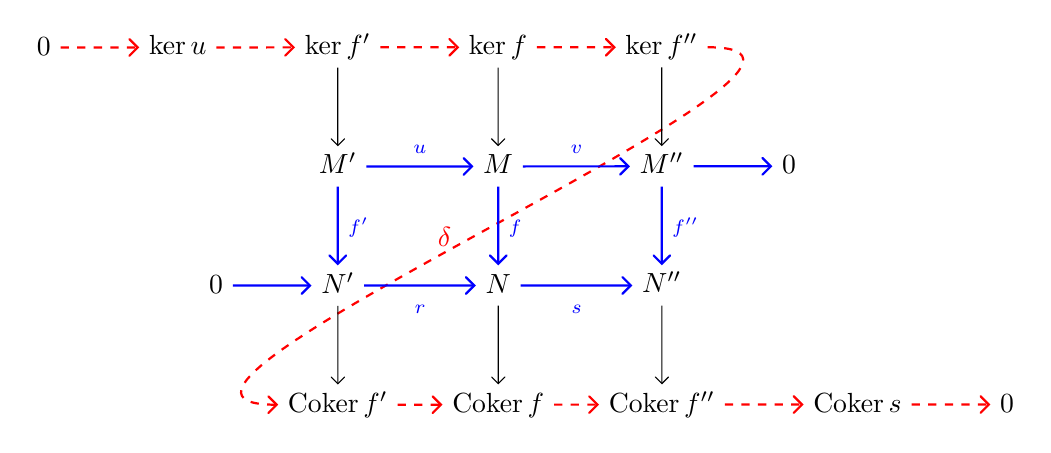
\begin{tikzpicture}[>=angle 90,scale=2.2,text height=1.5ex, text depth=0.25ex]
%%First place the nodes
\node (k-1) at (0,3) {$0$};
\node (k0) [right=of k-1] {$\ker u$};
\node (k1) [right=of k0] {$\ker f'$};
\node (k2) [right=of k1] {$\ker f$};
\node (k3) [right=of k2] {$\ker f''$};
\node (a1) [below=of k1] {$M'$};
\node (a2) [below=of k2] {$M$};
\node (a3) [below=of k3] {$M''$};
\node (a4) [right=of a3] {$0$};
\node (b1) [below=of a1] {$N'$};
\node (b0) [left=of b1] {$0$};
\node (b2) [below=of a2] {$N$};
\node (b3) [below=of a3] {$N''$};
\node (c1) [below=of b1] {$\Coker f'$};
\node (c2) [below=of b2] {$\Coker f$};
\node (c3) [below=of b3] {$\Coker f''$};
\node (c4) [right=of c3] {$\Coker s$};
\node (c5) [right=of c4] {$0$};
%%Draw the red arrows
\draw[->,font=\scriptsize,red,dashed,thick]
(k-1) edge (k0)
(k0) edge (k1)
(k1) edge (k2)
(k2) edge (k3)
(c1) edge (c2)
(c2) edge (c3)
(c3) edge (c4)
(c4) edge (c5);
%%Draw the curvy red arrow
\draw[->,red,dashed,thick]
(k3) edge[out=0,in=180,red] node[pos=0.55,yshift=5pt] {$\delta$} (c1);
%%Draw the black arrows
\draw[->]
(k1) edge (a1)
(k2) edge (a2)
(k3) edge (a3)
(b1) edge (c1)
(b2) edge (c2)
(b3) edge (c3);
%%Draw the thick blue arrows
\draw[->,font=\scriptsize,blue,thick]
(a1) edge node[auto] {$u$} (a2)
(a2) edge node[auto] {$v$} (a3)
(a3) edge (a4)
(a1) edge node[auto] {$f'$} (b1)
(a2) edge node[auto] {$f$} (b2)
(a3) edge node[auto] {$f''$} (b3)
(b0) edge (b1)
(b1) edge node[below] {$r$} (b2)
(b2) edge node[below] {$s$} (b3);
\end{tikzpicture}
\end{center}
\proof first note the all the vertical and horizontal lines are exact. We first consider the following construction:
\begin{enumerate}
  \item Start with $x''\in \ker f''$, which is mapped to $x''\in M''$
  \item choose $x\in M$ such that $v(x)=x''$. Apply $f$ , we have $y:f(x)\in N$.
  \item Choose(\textbf{Verify it we can choose indeed!}) that $y'\in N'$ such that $r(y')=y$ such that $y'$ is mapped to $y'\in \Coker(f')$.
  \item Define $\delta(x'')=y'$
\end{enumerate}
The following is left to the readers to show:
\begin{itemize}
  \item $\delta(x'')$ is well-defined.
  \item $\delta$ is indeed an $A$-module homomorphism.
  \item $\ker(r)=\im(\delta)$ and $\ker(\delta)=\im(v)$.i.e., the map is indeed exact.
\end{itemize}
\begin{noRmk}
One is to note that the aforementioned techniques is elementary in homology theory and respectively in homological algebra. Moreover, note the snake's lemma holds for \textbf{ANY ABELIAN CATEGORY}. The reader who has interest may consult the following article:\\
\textit{http://therisingsea.org/notes/DiagramChasingInAbelianCategories.pdf}
\end{noRmk}

 \medskip
Now we start our discussion in additive functors.
\Def Let $\mathcal{C}$ be a given collection of $A$-modules, Let $G$ be an abelian group. Then an \textbf{additive functor} in $\mathcal{C}$ is a any map $\lambda:\mathcal{C}\to G$ such that $\forall$ exact sequences:
\begin{equation}
  \begin{tikzcd}
    0\ar{r} &M'\ar{r} &M\ar{r} &M''\ar{r} &0
  \end{tikzcd}
\end{equation}
with $M', M, M''\in \mathcal{C}$, one has $\lambda(M)=\lambda(M)+\lambda(M'')$.
\Exe When $\mathcal{C}=$ all finite-dimensional vector spaces, then $\dim$ is an additive functor.
\Prop Let $0\to M_0\to M_1\to \cdots \to M_{n-1}\to M_n\to 0$ is exact and kernel of each homomorphism belong to $\mathcal{C}$ and each $M_i\in \mathcal{C}$, then for any additive functor $\lambda: \mathcal{C}\to G$, one has the \textbf{Euler characteristic} $\sum_{i=0}^n(-1)^i\lambda(M_i)$ is zero.
\proof Break the long exact sequence into the short exact sequence $0\to N_i\to M_i\to N_{i+1}\to 0$ for $i=0, ..., n$ using the previous trick, where $N_0=0=N_{n+1}$ and $N_i$ is kernel of some homomorphisms. Then $N_i\in \mathcal{C}$. Then $\forall i$, $\lambda(M_i)=\lambda(N_i)+\lambda(N_{i+1})$ by additive functor property, then $\sum_{i=0}^\infty (-1)^i\lambda(M_i)=\lambda(N_0)+(-a)^{n+1}\lambda(N_{n+1})=0$. Hence $\lambda(0)=\lambda(0)+\lambda(0)$  implies $\lambda(0)=0_G$.
\Def A \textbf{(finite) chain of submodule} of $M$ is a (finite) sequence of submodule $0=M_0\subsetneq M_1\subsetneq ...\subsetneq M_n=M$. We define the \textbf{length} of the chain to be the number of $\subsetneq$ involved.
\Def We define the above chain to be a \textbf{composition series} if it cannot be refined to a longer chain. i.e., we cannot insert more intermediate terms.
\Exe Consider $\z$ as a $\z$-module does not have composition series. Suppose to the contrary $0=M_0\subsetneq ...\subsetneq M_n=\z$ a composition series. Consider $M_{n-1}\subsetneq \z$ an abelian group, then $M_{n-1}=d\z$ for some $d\neq \pm1$. If $d=0$, then clearly $n\z$ is the intermediate term. If $d\neq 0$, then consider $M_{n-2}\subsetneq M_{n-1}$ which is $e\z$. The same logic applies, showing that $e\neq 0$. Consecutively applying it, either the series terminates, in which we yield a contradiction, or the series does not terminate.
\Exe On the other hand, any finite abelian group $G$ as a $\z$-module has a composition series, then by the structural theorem of abelian group the series $0\subsetneq p^{n-1}\z/p^n\z\subsetneq...\subsetneq \z/p^n\z$ is the desired composition for one component.
\Def An $A$-module $M$ has \textbf{finite length} if it has a composition series and we define the length to be the length of an choice of composition series.
\Rmk The well-definedness of the length of $M$ is substantiated via the following theorem:
\Theo [Jordan-H\"older theorem] Any two composition series of $M$ which has same length and has same isomorphism class of subquotients.
\Rmk The theorem endowed all the finite-length $A$-modules with another additive functor:
\begin{center}
  length:\{finite length $A$-module\}$\longrightarrow \z$
\end{center}
Now we return to exploit some properties of exact sequences.
\Prop If $M_1\overset{f}{\to}M_2\overset{g}{\to}M_3\to 0$ is exact $\iff$ for any $A$-module $N$, the following sequence is exact:
$$ 0\to \Hom(M_3, N)\overset{g^*}{\to} \Hom_A(M_2, N)\overset{f^*}{\to} \Hom_A(M_1, N)$$
\Rmk Note $f$ can behave as a homomorphism of abelian groups via a contravariant functor between $A$-modules and abelian groups as the following:
\begin{align*}
  \Hom_A(-, N):M&\mapsto \Hom_A(M, N)
\end{align*}
via the followings commutative diagram:
\begin{equation}
  \begin{tikzcd}
    M_1\ar{r}{f}\ar[dashed]{d}[swap]{f^*(\psi):=\psi\circ f} & M_2\ar{ld}{\psi}\\
    N
  \end{tikzcd}
\end{equation}

\medskip
In the spirit as above, we have the following:
\Prop If $0\to M_1\overset{f}{\to}M_2\overset{g}{\to}M_3$ is exact $\iff$ for any $A$-module $N$, the following sequence is exact:
$$ 0\to \Hom(N, M_3)\overset{f_*}{\to} \Hom_A(N, M_2)\overset{g_*}{\to} \Hom_A(M_1, N)$$
\Rmk Note here $f$ induces a morphism: $\Hom(N,M_1)\to \Hom(N, M_2), \quad \psi\mapsto f\circ\psi$. Essentially we have a functor again between $A$-module and abelian groups. $\Hom(N, -)$ which is covariant this time. Due to the symmetry in argument we shall only prove the second proposition:
\proof the $\Rightarrow$ direction is rather straightforward hence left to the reader. As for the $\Leftarrow$ direction:
\begin{enumerate}
  \item \textbf{$f$ is injective}: Take $N=\ker f$. So there is the natural inclusion $i:N\inj M_1$. i.e., $i\in \Hom(N, M_1)$. But $f_*(i)=f\circ i=0$. Hence by the injectivity of $f_*$ we have $i=0$. Thus $f$ injective.
  \item \textbf{$\im f=\ker g$}: take $N=M_1$. take $\phi=1_{M_1}\in \Hom(N, M_1)$, then $g_*f_*\phi=0\Rightarrow g\circ f \circ 1_{M_1}=0$. Hence $\im f\subseteq \ker g$. Take $N=\ker g\subseteq M_2$, let $i:N\inj M_2$ be natural inclusion, so $i\in \Hom(N, M_2)$, and $g\circ i=0$. Now by exactness, $i\in \im f_*$, i.e., $\exists \psi\in \Hom(N, M_1)$ such that $i=f\circ \psi$.
\end{enumerate}
\Rmk Alternatively for the second part of the proof above, we can take the test module to be $A$ directly. Moreover, we call $\Hom_A(-, N)$ and $\Hom_A(N, -)$ are \textbf{exact on the left}, in justifying that both of them acting on the exact sequence and produces a left-exact sequence.
\Def We define the $A$-module $N$ is \textbf{projective} (resp. \textbf{injective}) if $\Hom(N, -)$ (resp. $\Hom(-, N)$) is left-exact functor.

\bigskip
\subsection{Tensor product}
Given two $A$-modules $M$ and $N$, consider functors $f:M\times N\to P$. Then $f$ is an $A$-bilinear map if:
\begin{enumerate}
  \item  for any $n\in N$, $f(-, n)\in \Hom_A(M, P)$
  \item for any $m\in M$, $f(m, -)\in \Hom_A(N, P)$.
\end{enumerate}
Consider, $S_{M, N}=\{(P, f)| P \text{ is a }A\text{-module}; f:M\times N\to P \text{ bilinear}\}$. Note $S_{M,N}\neq 0$ since $(0, 0)\in S_{M, N}$.
\Prop [Universal property of tensor product] $\exists (T, i)\in S_{M, N}$ with the following universal property: Given any $(P, f)\in S_{M, N}$, $\exists !$ $A$-linear map $\bar{f}:T\to P$ such that $\bar{f}\circ i=f$, i.e., for any $P$, one has a canonical bijection:
\begin{center}
  \{Bilinear form $f:M\times N\to P$\}$\leftrightarrow$ $\Hom_A(T, P)$
\end{center}
Moreover, the pair $(T, i)$ is unique up to an unique isomorphism. In terms of commutative diagram, we have:
\begin{equation}
  \begin{tikzcd}
    M\times N \ar{r}{i} \ar{rd}[swap]{f} & T\ar[dashed]{d}{\exists !}[swap]{\bar{f}}\\
    &P
  \end{tikzcd}
\end{equation}
\proof Existence is proven henceforth. Uniqueness is proven replacing the test object $P$ by $T'$ and simultaneously applying the universal property to $T$ and $T'$, as always.\\Consider the free $A$-module $C$ generated by the following elements of $M\times N$, where $C$ consists of all formal finite linear combinations of $(m, n)\in M\times N$. A typical element in $C$ has the following form $\sum_{i=1}^n a_i(m_i, n_i)$. Analytically we may think $C$ as $$\{f: M\times N\to A|f \text{ with finite support}\}$$
Let $D\subseteq C$ the $A$-submodule generated by:
\begin{itemize}
  \item $(a_1m_1+a_2m_2, m)-a_1(m_1, m)-a_2(m_2, m)$;
  \item $(m, a_1m_1a_2m_2)-a_1(m, m_1)-a_2(m, m_2)$.
\end{itemize}
i.e., $D$ is the equivalent relations we wish to built up in $T$. Set $T=C/D$. Now we proceed to check $T$ fulfills universal property. Consider the following diagram:
\begin{equation}
  \begin{tikzcd}
    M\times N\ar{r}{i}\ar{d}{f}& T=C/D\ar[dashed]{ld}{\bar{f}}\\
    P
  \end{tikzcd}
\end{equation}
Uniqueness of $\bar{f}$ follows from image of $M\times N$ under $i$ generated $T$ as $A$-modules, so for all $(m, n)\in M\times N$, $\bar{f}$ is specified by $\bar{f}\circ i=f$. We hence define $\bar{f}:C\to P$ by $\bar{f}(m, n)=f(m, n)$. Then the $A$-bilinearity of $f$ implies that $D\in \ker \bar{f}$. Hence $\bar{f}$ factors through $D$, i.e, $C/D\overset{\bar{f}}{\to} P$.
\Def We set $M\otimes_A N$ to be the pair $(T, i)$ in the proposition above. Write the pair $(m, n)$ to be $m\otimes n$.
\Exe \leavevmode
\begin{itemize}
  \item $A=\z: \z/2\z\otimes_{\z} \z/3\z=0$, for $1\otimes 1=-2\otimes 1=0\otimes 1=0$.
  \item $\z\cdot 2=M_0\subseteq \z e:=M$, and $N=\z/2\z$. Then $M_0\otimes N=\z/2\z$, BUT $M\otimes N=0$.
  \item When $A=\field$ be a field and $M, N$ are finite-dimensional vector spaces over $\field$ with bases $\{m_i\}, \{n_j\}$ respectively. then $\{m_i\otimes n_j\}$ forms a basis of $M\otimes_\field N$. To prove this, $\dim_\field M\otimes_\field N\leq \dim_\field M\cdot \dim_\field N$ is easy to verify. To see the other side, note via universal property one has $\forall \field$-vector space $P$, $\Hom_\field(M\otimes N, P)\cong \{\field-\text{bilinear map}:M\times N\to P\}$. In particular, take $P=\field$, one has $M\otimes N^*\cong \{\field-\text{bilinear map}:M\times N\to \field\}$, which proves the assertion since $M$ and $N$ are finite-dimensional spaces.
\end{itemize}
Now we discover some properties of tensor product.
\begin{itemize}
  \item \textbf{Functoriality}. If $M_1\overset{f}{\to} M_2$ and $N_1\overset{g}{\to} N_2$, then:
  \begin{align*}
    M_1\otimes _A N_1&\overset{f\otimes g}{\longrightarrow} M_2\otimes_A N_2\\
    m_1\otimes n_1&\mapsto f(m_1)\otimes g(n_1)
  \end{align*}
  To verify  this, applying the universal property to $\Phi: M_1\otimes N_1\to M_2\otimes_AN_2, \quad (m,n)\mapsto f(m)\otimes g(n)$.
  \item \textbf{Canonical isomorphisms}
    \begin{enumerate}
      \item \textbf{"Commutativity"}:$M\otimes N\cong N\otimes M, \quad m\otimes n\mapsto n\otimes m$
      \item \textbf{Associativity}:$(M\otimes N)\otimes P\cong M\otimes(N\otimes P) \quad (m\otimes n)\otimes p\mapsto m\otimes(n\otimes p)$
      \item \textbf{Distributivity}: $(M\otimes N)\otimes P\cong M\otimes P\oplus N\otimes P, \quad (m, n)\otimes p\mapsto (m\otimes p, n\otimes p)$
      \item $A\otimes_A M\cong M, \quad a\otimes m\mapsto am$
      \item $\Hom(M\otimes N, P)\cong \Hom(M, \Hom(N, P))$
    \end{enumerate}
    \proof We shall only prove the last case. Note $$\Hom(M\otimes_A N, P)\cong \{\text{bilinear map:} M\times N \to P \}\cong \Hom(M, \Hom(N, P))$$.
\end{itemize}
\Prop If $M_1\to M_2\to M_3\to 0$ is exact, then for any $P$,
$$M_1\otimes P\to M_2\otimes P\to M_3\otimes P\to 0$$ is exact.
\proof Note this is straightforward from the previous proposition tensoring $N$ with a right-exact sequence, by taking $N$ to be $\Hom(P, Q)$ for any $Q$, then via the equality $\Hom(M_i, \Hom(P, Q))\cong \Hom(M\otimes P, Q)$, one yields the desired exactness.
\Rmk We have shown that:
$$-\otimes_A N: \{A-\text{modules}\}\to \{A-\text{modules}\} \quad M\mapsto M\otimes_A N$$
is right exact. Note the functor is not exact. When one takes $A=\z$ and $M_i=\z$ for all $i$, and $N=\z/2\z$. Then $0\to M_1\to M_2$ is exact, sending $m$ to $2m$. But the tensor product of the exact sequence, being $0\to \z/2\z\to \z/2\z$ is not exact, since it sends $x\otimes \mapsto 2x\otimes 1\cong x\otimes 2=0$.
\Def If $N$ is the $A$-module such that $-\otimes_A N$ is an \textbf{exact functor}, i.e., it is both left-exact and right-exact functor,  then $N$ is defined to be a \textbf{flat module}.

\medskip
The flat modules can be characterized by the following proposition:
\Prop Let $N$ be an $A$-module. Then the following are equivalent:
\begin{enumerate}
  \item $N$ is flat.
  \item $\forall$ short exact sequence, $0\to M'\to M\to M''\to 0$, the sequence $0\to M'\otimes N\to M\otimes N\to M''\otimes N$ is exact.
  \item $\forall$ injective $A$-module homomorphism $f:M'\to M$, the homomorphism $f\otimes 1_N:M '\otimes N\to M\otimes N$ is injective.
  \item (3) holds for all finitely generated $A$-modules $M', M$.
\end{enumerate}
\proof $(1)\iff (2)$ via breaking the long exact sequence to short ones, while $(2)\iff (3)$ was proven already.\\
$(3)\Rightarrow (4)$ is clear. For the other direction, given $u=\sum_i m_i'\otimes n_i\in \ker(f\otimes 1_N)$,hence $0=\sum_i f(m_i')\otimes n_i\in M'\otimes N$. Now let $M_0'$ be the submodule of $M'$ generated by $m_i'$ and $M_0$ be that of $M$ generated by $f(m_i)'$, both of which are finitely generated. Let $f_0$ be the restriction of $f: M'\inj M$ to $M'_0$ to $M_0'$, which means that $(f_0\otimes 1)(u_0)=0$. Since both $M_0$ and $M_0'$ are finitely generated, $f_0\otimes 1$ is injective by the presumption, hence $u_0=0$, which implies $u=0$.
\bigskip
\subsection{Algebras}
Recall the definition of $A$-algebras, we now consider the finitely generated algebras.
\Def $B$ is a \textbf{finitely generated $A$-algebra} if there is a finite subset $\Sigma\subseteq B$ such that $B$ is generated by b$A\cap \Sigma$ as a ring. This is equivalence to say, that $A[\Sigma]\surj B$. We say $B$ is a \textbf{finite $A$-algebra} if $B$ is finitely generated as an $A$-\textit{module}.
\Exe When $B=A[x]$ is a finitely generated $A$-algebra, but it is not finite, for it is free of infinite rank as $A$-module, while $C=A[x]/[x^3]$ is a finite $A$-algebra.

\medskip
Now suppose $M$ is an $A$-module, while $B$ an $A$-algebra. Since $B$ is naturally an $A$-module, one can form the $A$-module $M\otimes_A B\cong B\otimes_A M$. Then this $M\otimes_A B$ has a natural $B$-module structure: $b\cdot(b_1\otimes m_1)=(bb_1)\otimes m_1$.
\Def We call the aforesaid $B$-module $B\otimes_A M$ the \textbf{base change (or scalar extension)} of $M$ via $f:A\to B$.
\Exe When $f:\real\to \complex$. then $M$ as an $\real$-vector space and $\complex\otimes M$ is simply the complexification, sending $e_i\mapsto 1\otimes e_i$. More generally, if $M$ is generated by $\{m_i\}$, then $B\otimes_A M$ is generated as $B$-module by $\{1\otimes m_i\}$.

\medskip
Now consider if $B, C$ are both $A$-algebras and hence $A$-modules, then $B\otimes_A C$ has a natural ring/algebra structure, where the multiplication is $(b_1\otimes c_a)\cdot (b_2\otimes c_2)=(b_1b_2\otimes c_1c_2)$. first we check the map is well-defined: First consider the following $A$-multilinear map:
\begin{align*}
  B\times C\times B\times C&\to B\otimes_A C\\
  (b_1, c_1, b_2, c_2)&\mapsto b_1b_2\otimes c_1c_2
\end{align*}
which induces an $A$-bilinear map on $(B\otimes C)\otimes_A (B\otimes_A C)\to B\otimes_A C$, the "sub-multiplication" of which gives the desired multiplication in $B\otimes_A C$. Summarizing it, we have the following diagram:
\begin{equation}
  \begin{tikzcd}[row sep=small, column sep=small]
    &B\otimes_A C\\
    B\ar{ru} & &C\ar{lu}\\
    &A\ar{lu}{f_B}\ar[dashed]{uu}{f} \ar{ru}[swap]{f_C}
  \end{tikzcd}
\end{equation}
where $f(a)=f_B(a)1_B\otimes 1_C=1_B\otimes f_C(a)$. Motivated by such, the $A$-algebra $B\otimes_A C$ equipped with the algebra structure $f:A\to B\otimes_A C$ can be characterized by the following universal property:
\Prop For any $A$-algebra $D$ and a respective commutative diagram:
\begin{equation}
  \begin{tikzcd}[row sep=small, column sep=small]
    &D\\
    B\ar{rd}\ar{ru}{\phi_B} & &C\ar{ld}\ar{lu}[swap]{\phi_C}\\
    &B\otimes_A C\ar[dashed]{uu}{\exists !}[swap]{\phi}
  \end{tikzcd}
\end{equation}
$\exists ! \phi: B\otimes_AC\to D$ an $A$-algebra homomorphism.
\proof We leave it as an exercise to the readers to show this universal property. Note $\phi(b\otimes c)=\phi_B(b)\phi_B(b)\cdot \phi_C(c)$.
\Rmk Thus $B\otimes_A C$ is the "direct sum" of $B$ and $C$ in the category of $A$-algebra. When applying the functor "$\Spec$" to transfer it to the geometric side, we have $\Spec(B\otimes_A C)$, which is named as the \textbf{fiber product} of $\Spec B$ and $\Spec C$ over $\Spec A$ considering the following diagram:
\begin{equation}
  \begin{tikzcd}[column sep=small]
    &\Spec(B\otimes_A C)\ar{rd}\ar{ld}\\
    \Spec(B)\ar{rd}&\Spec(D)\ar[dashed]{u}{\exists !}\ar{r}\ar{l}\ar{d} &\Spec(C)\ar{ld}\\
    &\Spec(A)
  \end{tikzcd}
\end{equation}

\medskip
Suppose $A$ and $B$ are rings, then an \textbf{$(A, B)$-bimodule} is a set $M$ such that $M$ is both an $A$-module and a $B$-module and for all $a\in A, b\in B, m\in M$, we have $a(bm)=b(am)$.
\Exe If $f:A\to B$ and ring homomorphism. then $B$ is an $A$-algebra. Then any $B$-module $M$ has a obvious bi-module structure.
\Lemma If $A, B$ are rings, where $M$ is a $A$-module, $N$ is a $(A, B)$ -bimodule and $P$ is a $B$-module. Then $M\otimes_A N$ and $N\otimes_B P$ are $(A, B)$-module. Moreover, there is a canonical isomorphism
$$(M\otimes_A N)\otimes_B P\cong M\otimes_A(N\otimes_B P)$$
of $(A, B)$-bimodules.
\proof The $B$-module structure on $M\otimes_A N$ is given by $b\in B$, where $M_b:N\to N$ sending $n\mapsto b\cdot m$ is $A$-linear. then by functoriality, one has: $M\otimes A N to M\otimes_A N$ sending $m\otimes n\mapsto m\otimes b\cdot n$. Define
$$(M\otimes_A N)\otimes_B P \overset{f}{\to} M\otimes_A(N\otimes_B P)\overset{g^{-1}}{\to} (M\otimes_A N)\otimes_B P$$
Consider $f_p: M\otimes N\to M\otimes_A(N\otimes_B P)$ sending $(m,n)\mapsto m\otimes (n\otimes p)$. then $f_p$ induces a homomorphism from $M\otimes_A N$. Now define $f$ sends $(x, p)$ to $f_p(X)$ , then we have a $B$-bilinear map. $g$ is defined in a similar manner.
\Prop[Preserving flatness by base change] Suppose $M$ is a $A$-module, $B$ is an $A$-algebra. If $M$ is a flat $A$-module, then $B\otimes_A M$ is a flat $B$-module.
\proof Let $N:=B\otimes_A M$. Given $N_1\to N_2\to N_3$ exact, one needs to show $N_1\otimes_B N \to N_2\otimes_B N\to N_3\otimes_B N$ exact. Note $B, N, N_i$ are all $(A, B)$-bimodules, now the second sequence is obtained form the first via tensoring $M$, i.e.,
$$N_i\otimes_B N = N_i\otimes_B (B\otimes_AM)\cong N_i \otimes_A M$$
Now $M$ is flat, hence the second is exact sequence of $A$-modules, and hence a exact sequence of $B$-modules.

\bigskip
\subsection{Localization}
\Def Let $A$ be a ring. then $S\subseteq A$ is a \textbf{multiplicatively closed (mult-closed)} if $1\in S$ and $S$ is closed under multiplication.
\Exe \leavevmode
\begin{enumerate}
  \item $A$ is an integral domain. then $S=A\backslash \{0\}$ is mult-closed.
  \item Take $a\in A$, then $S=\{a^n: n\in \nat\}$ is mult-closed.
  \item Let $\mathfrak{p}\subseteq A$ be the prime ideal, then $S=A\backslash \mathfrak{p}$ is mult-closed.
\end{enumerate}
Note $S$ functions as a denominator in localization.
\Rmk Consider the set $A\times S$, we would like to endow the product with an equivalence relation. First consider $(a, s)\sim (b, t) \iff at=bs$. Nevertheless, the transitivity cannot be fulfilled unless $S$ has no zero divisor. Hence it gives the right definition:
$$(a, s)\sim ( b, t) \iff \exists u\in S: u(at-bs)=0$$
\Def Let $S^{-1}A$ be the set of equivalence classes with addition: $\frac{a}{s}+\frac{b}{t}=\frac{at+bs}{st}$ and multiplication: $\frac{a}{s}\cdot \frac{b}{t}=\frac{ab}{st}$, which makes $S^{-1}A$ into a ring. Moreover, there is a natural ring homomorphism:
$$f:A\to S^{-1}A \quad a\mapsto \frac{a}{1}$$
We call the quotient ring $S^{-1}A$ the \textbf{localisation of $A$ with respect to $S$}.
\Exe \leavevmode
\begin{enumerate}
  \item When $A$ is an integral domain, and $S=A\backslash \{0\}$. Then $S^{-1}A$ is the field of fractions of $A$.
  \item $S^{-1}A=\{0\} \iff 0\in S$
  \item $\mathfrak{p}\in A$ prime, $S=A\backslash \mathfrak{p}$ Then $S^{-1}A=:A_\mathfrak{p}$ the \textbf{localization of $A$ at $\mathfrak{p}$}
  \item $S=\{f^n: n\in \nat\}$, then $S^{-1}A=\{\frac{a}{f^n}:n\in \z, a\in A\}$ a \textbf{localization of $A$ away from $f$}.
\end{enumerate}
\Rmk It is straightforward that $\forall s\in S, f(s)\in S^{-1}A$ is a unit. Hence if $I\subseteq A$ is an ideal such that $I\cap S\neq \emptyset$, then the ideal of $S^{-1}A$ generated by $f(I)$ is indeed the whole ring.

The pair of $A\to S^{-1}A$ satisfy the following universal property:
\Prop [Universal property of localization] Consider the pair $\Sigma:=\{A\overset{\phi}{\to}B: \phi(S)\subseteq B^\times\}$. Note $f\in \Sigma$. Then given any $\phi:A\to B$ in $\Sigma$, $\exists ! \tilde{\phi}: S^{-1}A \to B$ such that the following diagram commutes:
\begin{equation}
  \begin{tikzcd}
    A\ar{rr}{\phi} \ar{rd}{f}& &B\\
    &S^{-1}A\ar[dashed]{ru}{\exists ! \tilde{\phi}}
  \end{tikzcd}
\end{equation}
\proof We shall only construct the existence. The well-definedness and uniqueness are left to the reader. Note $\tilde{\phi}(\frac{a}{s})=\tilde{\phi}(\frac{a}{1})\tilde{\phi}(\frac{1}{s})$.

\medskip
Now we shift to discuss the localization of $A$-module. Let $S\subseteq A$, and $M$ is an $A$-module. Consider $M\times S$ and define equivalence relation
$$(m_1, s_1)\sim(m_2, s_2) \iff \exists t\in S: t(s_2m_1-s_1m_2)=0$$
\Def We define the \textbf{localization of $A$-module ar $S$} to be $S^{-1}M=M\times S/\sim$.
\Exe \leavevmode
\begin{enumerate}
  \item $S=\{f^n:n\in \nat\}$. Then $S^{-1}M=M_f$.
  \item $S=A\backslash \mathfrak{p}$, then $S^{-1}M=M_\mathfrak{p}$.
\end{enumerate}
Observe that $S^{-1}M$ are $S^{-1}A$-module with conventional addition and multiplication. Then if $\phi:M\to N$ is an $A$-module homomorphism, then it inherits an $S^{-1}A$-module homomorphism:
\begin{align*}
  S^{-1}\phi:S^{-1}M &\to S^{-1}N\\
  \frac{m}{s}&\mapsto \frac{\phi(m)}{s}
\end{align*}
Moreover, $M\overset{\phi}{\to} N\overset{\psi}{\to} P$, then we have $S^{-1}\phi\circ S^{-1}\psi:S^{-1}M\to S^{-1}N\to S^{-1}P$. That is:
\Def $M\to S^{-1}M$ is a functor from $A$ -module to $S^{-1}A$-module, which is defined as \textbf{localization functor}.

\medskip
We now discuss the basic properties of localization.
\begin{enumerate}
  \item $S^{-1}M\cong S^{-1}A\otimes_A M, \quad \frac{am}{s} \mapsto \frac{a}{s}\otimes m$. To see this , note $(\frac{a}{s}, m) \mapsto \frac{a}{s}$ is $A$-bilinear, which induces the map upon tensor product. To prove the injectivity, note if $\sum_i\frac{a_im_i}{s_i}=0$, set $\prod_i s_i=s, \prod_{j\neq i} s_j=t_i$, we conclude: $\exists u\in S: u(\sum_ia_it_im_i)=0\in M$. Hence $\frac{a_i}{s_i} \otimes m_i=\sum_i \frac{a_it_i}{s}\otimes m_i=\frac{1}{s}\otimes (\sum_i a_it_im_i)=\frac{1}{su}\otimes u(\sum_i(a_it_im_i))=0$.
  \item \textbf{localization is exact}: If $M_1\overset{\phi}{\to} M_2\overset{\psi}{\to} M_3$ is exact, then $S^{-1}M\overset{S^{-1}\phi}{\to} S^{-1}M_2\overset{S^{-1}\psi}{\to} S^{-1}M_3$ is exact.  Note since $\psi\circ \phi=0$ , then $S^{-1}\psi\circ S^{-1}\phi=0$,. Conversely, given $\frac{m_2}{s}\in S^{-1}M_2$ such that $S^{-1}\phi(\frac{m_2}{s})=0$. sp $\exists t\in S$ such that $t\cdot \psi(m_2)=0$. So $tm_2\in \ker \psi=\im \phi$. Then $\frac{m_2}{s}=S^{-1}\phi(\frac{m_1}{ts})$. i.e., $\ker(S^{-1}\psi)=\im(S^{-1}\phi)$.
  \item If $N, P\subseteq M$ are sub-$A$-module, then:
  \begin{enumerate}
    \item $S^{-1}(N+P)=S^{-1}N+S^{-1}P$
    \item $S^{-1}(N\cap P)=S^{-1}N\cap S^{-1}P$
    \item $S^{-1}(\frac{M}{N})=\frac{S^{-1}M}{S^{-1}N}$
  \end{enumerate}
  \item \textbf{localization commutes with tensoring}:
  \begin{align*}
    S^{-1}(M\otimes_A N)&\cong S^{-1}M \otimes_{S^{-1}A} S^{-1}N\\
    \frac{1}{st}m\otimes n&\leftarrow \frac{m_1}{s}\otimes \frac{n}{t}\\
    \frac{m\otimes n}{s}&\rightarrow \frac{1}{s}m\otimes n
  \end{align*}
  alternatively, $S^{-1}M\otimes_{S^{-1}A} S^{-1}N=(S^{-1}A\otimes_A M)\otimes_{S^{-1}A}(S^{-1}N)\cong M\otimes_A (S^{-1}A\otimes_{S^{-1}A}S^{-1}N)=M\otimes_A(N\otimes_A S^{-1}A)=(M\otimes_A N)\otimes_A S^{-1}A=S^{-1}(M\otimes_A N)$.
\end{enumerate}
\Cor $S^{-1}A$ is a flat $A$-module.
\proof Use (1) and (2) of the basic properties above.
Now we consider this local behaviour in a more general scope.
\Def Suppose $P$ is  a property of modules. Then we say $P$ is a \textbf{local property} if an $A$-module $M$ satify $P$ $\iff$ $\forall \mathfrak{p}\in \Spec A, M_\mathfrak{p}$ satisfy $P$ as a $A_\mathfrak{p}$-module.

\medskip
Firstly \textbf{Vanishing is a local property}.
\Prop the following are equivalent:
\begin{enumerate}
  \item $M=0$
  \item $M_\mathfrak{p}=0 \quad\forall \mathfrak{p}\in \Spec A$
  \item $M_\mathfrak{m}=0 \quad \forall$ maximal ideal $\mathfrak{m}\subseteq A$
\end{enumerate}
\proof (1)$\to$ (2)$\to$ (3) is clearly. Now assume the last, take $m\in M$, suppose $m\neq 0$, then consider $\Ann_A(m)=\{a\in A:am=0\}$ is an ideal in $A$. Note $m\neq 0$ implies $\exists$ a maximal ideal $\mathfrak{m}\supseteq \Ann_A(m)$. But then $m\neq-$ in $M_\mathfrak{m}$, which is  a contradiction, since this implies $\forall a\in A\backslash \mathfrak{m}, am\neq 0$.
\Cor the following are equivalent:
\begin{enumerate}
  \item $\phi:M\to N$ is injective.
  \item $\phi_\mathfrak{p}: M_\mathfrak{p}\to N_\mathfrak{p}$ is injective $\forall \mathfrak{p} \in \Spec A$.
  \item $\phi_\mathfrak{m}: M_\mathfrak{m}\to N_\mathfrak{m}$ is injective $\forall$ maximal ideal $\mathfrak{m}$.
\end{enumerate}

\medskip
Secondly \textbf{Flatness is a local property}.
\Prop The following are equivalent:
\begin{enumerate}
  \item $M$ is flat.
  \item $M_\mathfrak{p}$ is flat $\forall \mathfrak{p}\in \Spec A$.
  \item $M_\mathfrak{m}$ is flat $\forall$ maximal ideal $\mathfrak{m}$.
\end{enumerate}
\proof From $(1)\to (2)$. Suppose $(*):N_1\to N_2\to N_3$ is a exact sequence of $A_\mathfrak{p}$-module. We want to show $(**):N_1\otimes_{A_\mathfrak{p}}M_\mathfrak{p}\to N_2 \otimes_{A_\mathfrak{p}}M_\mathfrak{p}\to N_3\otimes_{A_\mathfrak{p}}M_\mathfrak{p}$ is exact. But note $(*)$ is exact as $A_\mathfrak{p}$-modules $\iff$ it is exact as $A$-modules $\iff (*) \otimes_A M$ is exact as $A$-modules. Now note $N_1\otimes_{A_\mathfrak{p}}M_\mathfrak{p}=N_1\otimes_{A_\mathfrak{p}}(A_\mathfrak{p}\otimes_A M)=N_1\otimes_A M$. Hence (*) $\otimes_{A_\mathfrak{p}} M_\mathfrak{p}$ is exact as $A_\mathfrak{p}$-module.\\
As for $(3)\to (1)$, It suffices to show: if $0\to N\to P$ is exact, then $0\to N\otimes_A M\to P\otimes_A M$ is exact. Note $N\to P$ is injective $\Rightarrow$ $N_\mathfrak{m}\to M_\mathfrak{m}$ is injective. Hence by the assumption, we have $N_\mathfrak{m}\otimes_{A_\mathfrak{m}}M_\mathfrak{m}\to P_\mathfrak{m}\otimes_{A_\mathfrak{m}}M_\mathfrak{m}$ is injective. Now $N_\mathfrak{m}\otimes_{A_\mathfrak{m}}M_\mathfrak{m}\cong (N\otimes_A M)_\mathfrak{m}$, so is $P_\mathfrak{m}\otimes_{A_\mathfrak{m}}M_\mathfrak{m}\cong (P\otimes_A M)_\mathfrak{m}$. Then by previous proposition, we have $N\otimes_A M\to P\otimes_A M$ is injective. \qedhere

\medskip
We shall now consider the properties of ideals. Consider $f:A\to S^{-1}A$ sending $a$ to $\frac{a}{1}$. We have the following diagram:
\begin{equation}
  \begin{tikzcd}[column sep=large]
  I \ar[|->]{r}{f^{-1}} & f^{-1}(I)\\
\{\text{ideals of }S^{-1}A\}\ar[bend left]{r}{f^{-1}=f^*} &\{\text{ideals of }A\}\arrow[bend left]{l}{S^{-1}}\\
 f(\mathfrak{a})\cdot S^{-1}A & \mathfrak{a}\ar[|->]{l}{S^{-1}}
  \end{tikzcd}
\end{equation}
Note $f(\mathfrak{a})\cdot S^{-1}A\cong S^{-1}\mathfrak{a}\cong S^{-1}A\otimes_A \mathfrak{a}$.
\Rmk If $\mathfrak{a}\cap S\neq \phi$, then $S^{-1}\mathfrak{a}=S^{-1}A$, hence $S^{-1}$ is not injective.
\Prop \leavevmode
\begin{enumerate}
  \item $S^{-1}\circ f^{-1}=1$. In particular, $f^{-1}$ is injective, $S^{-1}$ is surjective.
  \item $f^{-1}\circ S^{-1}(\mathfrak{a})=\{x\in A|x\cdot s\in \mathfrak{a}\text{ for some }s\in S\} \quad \forall \mathfrak{a}\in A$. Hence $S^{-1}\mathfrak{a}=S^{-1}A \iff \mathfrak{a}\cap S\neq \emptyset$.
  \item $f^{-1}$ and $S^{-1}$ induces bijection upon the sets: $\{\mathfrak{p}\in \Spec(A): \mathfrak{p}\cap S=\emptyset\}\leftrightarrow \{\Spec S^{-1}A\}$
\end{enumerate}
\Rmk Assuming the above proposition, we consider the map $f:A\to A_\mathfrak{p}$ which induces the injective $f^{-1}: \Spec A_\mathfrak{p}\overset{f^{-1}}{\inj}\Spec A_\mathfrak{p}$. Hence $\im(f^{-1})=\{\mathfrak{q}\in \Spec(A)|\mathfrak{q}\subseteq \mathfrak{p}\}$.
\proof \leavevmode
\begin{enumerate}
  \item Given $\mathfrak{b}\in S^{-1}A$ a prime ideal, then $S^{-1}(f^{-1}(\mathfrak{b}))\subset \mathfrak{b}$. Conversely, if $\frac{a}{s}\in \mathfrak{b}$, then $\frac{a}{1}=f(a)\in \mathfrak{b}$. Hence $a\in f^{-1}(\mathfrak{b})$ and $\frac{a}{s}\in S^{-1}(f^{-1}(\mathfrak{b}))$.
  \item First note:
  \begin{align*}
  x\in f^{-1}(S^{-1}\mathfrak{a}) &\iff f(x)\in S^{-1}\mathfrak{a}\iff \frac{x}{1}=\frac{a}{s}\text{ for some }a\in \mathfrak{a}, s\in S \\
    &\iff t(xs-a)=0 \text{ for some }t\in S \iff stx\in \mathfrak{a}\text{ for some }t\in S.
  \end{align*}
  Now it left to show if $S^{-1}\mathfrak{a}=S^{-1}A$ implies $\mathfrak{a}\cap S\neq \emptyset$. Note if $f^{-1}(S^{-1}A)=A$ then $1\in f^{-1}(S^{-1}\mathfrak{a})$, then $\exists s\in S$ such that $1\cdot s\in \mathfrak{a}$.
  \item If $\mathfrak{p}\in \im(F^{-1})$, say $\mathfrak{p}=f^{-1}\mathfrak{q}$, then $\mathfrak{p}\cap S=\emptyset$. Else $S^{-1}\mathfrak{p}=S^{-1}A$, where $S^{-1}(f^{-1}(\mathfrak{q}))=\mathfrak{q}$. So $f^{-1}:\Spec S^{-1}A\to \{\mathfrak{a}\in \Spec A|\mathfrak{a}\cap S=\emptyset\}$. We now want to show $S^{-1}\mathfrak{a}$ is prime. To prove it, note $S^{-1}A/S^{-1}\mathfrak{a}\cong S^{-1}(A/\mathfrak{a})$ where $A/\mathfrak{a}$ is an integral domain. Finally, $f^{-1}(S^{-1}\mathfrak{a})=\mathfrak{a}$ by (2).
\end{enumerate}
\Rmk Consider $f:A\to A_\mathfrak{p}, \quad \Spec(A)\overset{f^{-1}}{\hookrightarrow} \Spec A_\mathfrak{p}=\{\mathfrak{q}A_\mathfrak{p}:\mathfrak{q}\subseteq \mathfrak{p}\}$. Note $\mathfrak{q}A_\mathfrak{p}\subset \mathfrak{p}A_\mathfrak{p}$. In particular,  $\mathfrak{p}A_\mathfrak{p}$ is the unique maximal ideal in $A_\mathfrak{p}$. This give rises to the following definition:
\Def We define a ring $A$ to be a \textbf{local ring} if $A$ has a unique maximal ideal $\mathfrak{m}$. We further define the field of fraction $\field=A/\mathfrak{m}$ to be the \textbf{residue field of $A$}.
\Exe Given any $A$, $\mathfrak{p}\in \Spec A$, then $A_\mathfrak{p}$ is a local ring. In particular, $A=\z$ and $\mathfrak{p}$ is prime ideal of $A$. Then $A_\mathfrak{p}=\{\frac{m}{n}: p\nmid n\}$, in which the unique maximal ideal $\mathfrak{m}-\{\frac{pm}{n}: p\nmid n\}$.
\Exe The following example is itself of some significance in the realm of functional analysis. Recall $C(X)$, in which $X$ is a topological space. We take $x_0\in X$, then $\mathfrak{m}_{x_0}=\{f\in C(X)|f(x_0)=0\}$ is the maximal ideal of $C(X)$. To se this , consider the following diagram:
\begin{equation}
  \begin{tikzcd}
    f\ar[|->]{r}{\ev_{x_0}}&f(x_0)\\
    C(X) \ar{r}{\ev_{x_0}} \ar{d}& \real\\
    C(X)/\mathfrak{m}_{x_0}\ar[dashed]{ru}{\cong}
  \end{tikzcd}
\end{equation}
Then $C(X)\mathfrak{m}_{x_0}=\{f/g: f, g\in C(X), g\notin \mathfrak{m}_{x_0}\}/\sim$, where the equivalence relation is defined by:
$$f_1/g_1\sim f_2/g_2 \iff \exists g_3\notin \mathfrak{m}_{x_0}, (g_2f_1-f_2g_1)g_3=0$$
i.e., $C(X)\mathfrak{m}_{x_0}=\{(U, f): U$ is a neighbourhood of $x_0, f: U\to \real$ continuous$\}/\sim$. Note in this scenario, $(U_1, f_1)\sim(U_2, f_2) \iff \exists$ neighbourhood $V\subseteq U_1\cap U_2$ which contains $x_0$, such that $f_1|_V=f_2|_V$.
Hence $C(X)\mathfrak{m}$ is a local ring with unique maximal ideal $\{(U, f): f(x_0)=0\}$.
\Rmk Note in this example, we have degraded the global property, i.e., the continuity upon the whole space, to some local property on neighbourhood, the tactic of which is commonly used and are none the less of great significance in mathematics.
\Lemma $\mathfrak{m}\subseteq A$ is a maximal ideal. Then: $A$ is local $\iff \forall x\in A\backslash \mathfrak{m}$ are unit $\iff$ $\forall x\in \mathfrak{m}$, $1+x$ are units.
\proof The first $\iff$ is easy to prove and is hence handed to the readers. To see the second $\iff$, take $x\in A\backslash \mathfrak{m}$, we want to show $y\in A^\times$, but since $\mathfrak{m}$ and $x$ generates the whole ring, thus $ax+y=1$ for some $a\in A$ and $y\in \mathfrak{m}$. i.e., $ax=1-y\in A^\times \Rightarrow x\in A^\times$.

\medskip
We now proceed to state a useful yet easily stated lemma:
\Lemma [Nakayama's Lemma] Let $A$ be a local ring, in which $\mathfrak{m}$ the maximal ideal. Let $\field$ be the residue field. Let $M$ be a finitely generated $A$-module, consequently $M/\mathfrak{m}M$ is a finite dimensional $\field$-vector space. Hence suppose $\{x_i\}\subset M$ is a basis of $M/\mathfrak{m}M$, then $\{x_i\}$ generates $M$ as a module.
\Rmk This lemma essentially states that the basis of the quotient ring controls the behaviour of the whole (rather strictly confined) ring.
\proof Let $N$ be the submodule spanned by $\{x_i\}$, we want to show $M=N$. Note $\mathfrak{m}\cdot M/N=M/N$. Since $M=\mathfrak{m}M+N$. Hence it remains to show if $\mathfrak{p}$ is a finitely generated $A$-module with $\mathfrak{m}\mathfrak{p}=\mathfrak{p}$, then $\mathfrak{p}=0$. To prove this, choose a minimal set of generators $\{u_1, ..., u_n\}$, then $u_n=\sum_i^n x_iu_i$ for $x_i\in \mathfrak{m}$. then $(1-x_n)\cdot u_n=\sum_i^{n-1}x_iu_i$. But observe that $1-x_n$ is a unit by the above proposition, hence the minimality is contradicted.
\Rmk In an alternative way, we have the following version of Nakayama's lemma:
\Lemma [Nakayama's lemma, version 2] If $M$ is a finite $A$-module, and $\mathfrak{a}$ is an ideal lies inside $\bigcap$ all maximal ideals of $A$, i.e., $\mathfrak{a}$ is a subset of \textbf{Jacobson radical}, then $a\cdot M=M$ implies $M=0$.

\pagebreak
\section{Homological algebra}
\subsection{Injective and Projective module}
\Def An $A$-module $P$ is defined to be \textbf{projective} if $\forall$ exact sequence $\cdots\to M_1\to M_2\to \cdots$, the sequence $\cdots\Hom(P, M_1)\to \Hom(P, M_2)\to \cdots$ is exact.
\Rmk Note the snake's lemma gives us the freedom to redefine the above terms using short exact sequences, i.e., $\forall$ short exact sequence $0\to M'\to M\to M''\to 0$, the corresponding sequence in $\Hom(P, -)$ is exact. Note the functor $\Hom(P,-)$ is covariant.
\Prop[characterization of projective module] For an $A$-module $P$, the following are equivalent:
\begin{enumerate}
  \item $P$ is projective module
  \item every surjective module homomorphism $g:M\surj M'$ and every module homomorphism $f: P \to M$, $\exists$ a homomorphism $h : P \to M' $ such that the following diagram commutes:
      \begin{equation}
        \begin{tikzcd}
          & P\ar[dashed]{ld}{h}\ar{d}{f}\\
          M\ar[->>]{r}{g} &M''
        \end{tikzcd}
      \end{equation}
      i.e., every $f$ emanating from $P$ can be lifted via the surjective homomorphism.
  \item Any exact sequence $0\to M'\to M\to P\to 0$ splits.
  \item $\exists A$-module $P_0$ such that $P\oplus P_0$ is a free $A$-module.
\end{enumerate}
\proof For $(1)\Rightarrow (2)$, consider $M''$ to be the kernel of $g:M\to M'$, then $0\to M''\to M\to M'\to 0$ is clearly exact, hence by definition, we have:
$$0\to \Hom(P, M'')\to \Hom(P, M) \to \Hom(P, M'')\to 0$$
is exact. Hence $\exists h\in \Hom(P, M)$ such that $g\circ h=f$.\\
$(2)\Rightarrow (3)$, consider the following diagram:
\begin{equation}
  \begin{tikzcd}
    0\ar{r} &M''\ar{r} &M \ar{r} &M\ar{r} &0 \\
    & & &P\ar[dashed]{lu}{h}\ar{u}[swap]{\id_P}
  \end{tikzcd}
\end{equation}
The sequence splits via the lifted map.\\
$(3)\Rightarrow(4)$: Consider $f: F\surj P$ with kernel $P_0$. Then by the splitness we have $F\cong P_0\oplus P$.\\
$(4)\Rightarrow (1)$: If $P\oplus P_0\cong F$, where $F$ is free, then for any $M$, $\Hom(F, M)\cong \Hom(P, M)\oplus \Hom(P_0, M)$. Now If $\psi: M_1\to M_2$ is an homomorphism, then $\psi\circ -:\Hom(F, M_1\to \Hom(F, M_2)$ is constructed in an canonical way, where it is easy to verify that $\Hom(P, -)$ preserves exactness. Hence $P$ is projective.

\medskip
In a rather symmetric way, we shall define injective modules.
\Def An $A$-module $Q$ is defined to be \textbf{injective} if $\forall$ exact sequences $\cdots \to M_1\to M_2\to\cdots$, the corresponding sequence $\Hom(-, Q)$ is also exact. Note here $\Hom(-, Q)$ is a contracovariant functor.
\Rmk In the same fashion, the aforesaid definitions can be reformulated in terms of short exact sequences. i.e, if $)\to M'\to M\to M''\to 0$ is exact,then so is $0\to \Hom(M'', Q)\to \Hom(M, Q)\to \Hom(M', Q)$.
\Prop [Characterization of injective modules] For an $A$-module $Q$, the following are equivalent:
\begin{enumerate}
  \item $Q$ is injective.
  \item For any injective homomorphism $g: M'\inj M$ and any homomorphism $f: M'\to Q$, the following diagram commutes:
    \begin{equation}
      \begin{tikzcd}
        M'\ar{d}{f}\ar[hook]{r}{g} &M\ar[dashed]{ld}{h}\\
        Q
      \end{tikzcd}
    \end{equation}
  \item Every short exact sequence $0\to Q\to M\to M''\to 0$ splits.
\end{enumerate}
\proof The proof of the previous proposition carries over verbatim to this.
\Prop A $\z$-module is $Q$ injective $\iff$ it is \textbf{divisible}, that is, $$\forall m\in \z\backslash\{0\},\text{ the map }\cdot \circ m:Q\to Q; \quad x\mapsto mx $$is surjective.
\proof First prove the $\Rightarrow$ direction. Suppose $Q$ is not divisible. Then $\exists m\in \z\backslash\{0\}$ and $y\in Q$ such that $\forall x\in Q$ such that $y\neq mx$. Consider the following diagram where $f:\z\to Q$ maps $1$ to $y$ and $m$ maps $a$ to $ma$. Then by $Q$ being injective module there induces an map $g$:
\begin{equation}
  \begin{tikzcd}
    \z\ar[hook]{r}{m}\ar{d}{f}&\z\ar[dashed]{ld}{g}\\
    Q
  \end{tikzcd}
\end{equation}
Then clearly $y=f(1)=g(m)=m\cdot g(1)=mx$, a contradiction.\\
As for the $\Leftarrow$ side, suppose $Q$ is divisible. Then we first show this is true for $M':=M+\z x$, where $x\in M$. then inductively we attach other elements. If $\z x\cap M'=0$, then $M=M'\oplus \z x$, in which case we define $h(m=m'+lx)=f(m')+l\cdot 0$, hence the homomorphism $h:M\to Q$ works. If on the other hand,  $\z \cdot x\cap M'\neq 0$, then we can pick the smallest $d\in \z_{>0} $ such that $d\cdot x\in M'$, then by divisibility of the module we could always found a $u\in Q$ such that $d\cdot u=f(dx)$.Now define:
\begin{align*}
  h:M&\to Q\\
  m=m'+lx&\mapsto f(m')+lu
\end{align*}
Verify that $h$ is a well-defined map, in which the assumption that $d$ is the smallest element shall be used. Also verify that this $h$ as a $\z$-homomorphism makes the following diagram commutes:
\begin{equation}
  \begin{tikzcd}
    x\in M'+\z\cdot x=M\ar[dashed]{r}{h} &Q\ar[->>]{d}{\cdot d}\\
    d\cdot x\in M'\ar[hook]{u}\ar{r}{f} &Q\ni f(dx)
  \end{tikzcd}
\end{equation}
As for general $M$, one can consider the set of $(N, g)$ where $M'\subseteq N\subseteq M$ as a module and $g:N\to Q$ making the following commutes:
\begin{equation}
  \begin{tikzcd}
    M\ar[hook]{r}\ar{d}{f} &N[\ar{ld}{g}\ar[hook]{r}&M]\\
    Q
  \end{tikzcd}
\end{equation}
Note this set is partially ordered by the binary relation:
$$(N, g)\preceq (N', g')\quad \iff \quad N\subseteq N', g=g'|_N$$
Now clearly this family is upper bounded by $\bigcup_i N_i$, hence applying Zorn's lemma we yield a maximal element $(N, g)$. We claim $N=M$. Suppose if not, then choose $x\in M\backslash N$, we consider $\tilde{N}:=N+\z x\subseteq M$, which is the larger than $N$.
\Exe $\rat$ and $\rat/\z$ are both divisible, hence injective.

\medskip
If $A$ is PID, $K\subset Frac(A)$. The proof requires the splitting the exact sequence of :
\begin{equation}
  \begin{tikzcd}
    A^\times \ar[hook]{r}&K^\times \ar[two heads]{r} &\{\text{Group of non-zero ideals in }K\} \ar[bend right,dashed]{l}
  \end{tikzcd}
\end{equation}
\Prop For any ring $A$, $A$ module $M$, there os a canonical isomorphisms of $\z$-module between $A$-module $M$ and $\z$-module $T$:
\begin{equation}
\begin{tikzcd}[row sep=tiny]
    \Hom_\z(M, T) \ar[<->]{r}{\cong} &\Hom_A(M, \Hom_\z(A, T))\\
  \psi\ar[|->]{r}&(m\mapsto (a\mapsto \psi(am)))\\
  (m\mapsto f(m)(1_A)) &f\ar[|->]{l}
\end{tikzcd}
\end{equation}
\proof Routine check.
\Prop Suppose $T$ is divisible $\z$-module (and hence injective as a $\z$-module), then $\Hom_\z(A, T)$ is injective as $A$-module.
\proof We want to see $\Hom_A(-, \Hom_\z(A, T))$ is a right exact functor. But via using the previous proposition, this sums up to show $\Hom_\z(-, T)$ is exact. But $T$ is an injective abelian group.

\medskip
With all these preparations, we can now prove the main theorem:
\Theo Given any $A$-module $M$, $\exists$ injective $A$-module $Q$ and an injective homomorphism $M\inj Q$.
\proof Given $A$-module $M$, which we first regard $M$ as an abelian group, we can choose a divisible abelian group $T$ and injective abelian group homomorphism: $f: M\inj T$. To see this, consider $F:=\z^{\oplus S}$  be any free abelian group, then
$$\Hom_\z(F, \rat/\z)\cong \prod_{s\in S}(\rat/\z)$$
is an injective $\z$-module. then for any abelian group $X$, we denote $X^\vee:=\Hom_\z(X, \rat/\z)$, one yield $X^{\vee\vee}=\Hom_\z(X^\vee, \rat/\z)$, hence there is a canonical homomorphism:
\begin{align*}
  X&\to X^{\vee\vee}\\
  x &\mapsto (\psi \mapsto \psi(x))
\end{align*}
which is injective.  Now given $X$ and $X^\vee$, choose free abelian group $F$ and surjective homomorphism $F\surj X^\vee\to 0$. Apply $\Hom_\z(-, \rat/\z)=(-)^\vee$. Hence we get $0\to X^{\vee\vee}\inj F^\vee$, so we show $X$ can be embedded in side a injective abelian group of $F^\vee$.\\
Now to see the full version, consider $M$ as stated in proposition. Then $0\to M\overset{\psi}{\to} T$. So $\psi\in \Hom_\z(M, T)$ $\iff$ $f:=(m\mapsto (a\mapsto \psi(am)))\in \Hom_A(M, \Hom_\z(A, T))$. Hence $M\to \Hom_\z(A, T)$ is a $A$-module homomorphism, the later of which is an injective $A$-module. Verify $f$ is injective, we then obtain the desired result.

\bigskip
\subsection{Ext and Tor functors for $A$-module}
Given any pair of $A$ module $M, N$, then $\forall n\in \nat$, $\exists$ an $A$-module (or resp. $\Tor_n^A(M, N)$). Fix $M$, and for all short exact sequence $0\to N'\to N\to N''\to 0$, one has the long exact sequence:
\begin{equation}
  \begin{tikzcd}
    0\ar{r} &\Hom_A(M, N') \ar{r} & \Hom_A(M, N) \ar{r} &\Hom_A(M, N'')\ar{lld}\\
    &\Ext_A^1(M, N') \ar{r} &\Ext_A^1(M, N) \ar{r} &\Ext_A^1(M, N'')\ar{lld}\\
    &\Ext_A^2(M, N') \ar{r} &\cdots
  \end{tikzcd}
\end{equation}
 and resp. the long exact sequence:
 \begin{equation}
   \begin{tikzcd}
     &\cdots \ar{r} &\Tor_2(M, N'')\ar{lld}\\
     \Tor_1(M, N') \ar{r} &\Tor_1(M, N) \ar{r} &\Tor_1(M, N'')\ar{lld}\\
     M\otimes N'\ar{r} &M\otimes N \ar{r} &M\otimes N''\ar{r} &0
   \end{tikzcd}
 \end{equation}
 i.e., we can see $\Ext_A^0=\Hom_A$, and $\Tor_0=-\otimes-$.

 \medskip
 Having seen this abstract and a bit void definition, we see how to construct $\Ext^n(M, N)$ in concrete ways. The first way is to fix $M$ first. Then for any $A$-module $N$, we want the family of $A$-module $\{\Ext^n(M, N)\}_{n\in \nat}$ and $\forall$ homomorphism $N\to N''$, we want $A$-module homomorphism $\Ext^n(M, N)\to \Ext^n(M, N'')$ and for all short exact sequence $0\to N'\to N\to N''\to 0$, we want $A$-module homomorphism $\Ext^n(M, N'')\to \Ext^{n+1}(M, N')$ such that the exactness holds.

 \medskip
 To construct this, we first start with $N$. Use the fact that $\exists $ enough injective $A$-modules, one gets $0\to N\overset{j_0}{\to} Q^0$ where $Q^0$ is an injective $A$-module. Now get $\Coker j_0$, we get $\Coker(j_0)\inj Q'$, where $Q'$ is injective $A$-module. Hence$0\to N\overset{j_0}{\to} Q^0\overset{j_1}{\to} Q'$ exact. continuing the process, one yields the long exact sequence with each $Q^i$ injective $A$-module.

 \medskip
 Now apply $\Hom_A(M, -)$ to everything. Hence $\Hom_A(M, N)$ gives an complex (which is not exact in general):
 $$\Hom_A(M, Q^0)\overset{j_1\circ-}{\to} \Hom_A(M, Q^1)\overset{j_2\circ-}{\to} \Hom_A(M, Q^2)\overset{j_3\circ-}{\to} \cdots$$

 Now define $\Ext_A^n(M, N)$ to be the $n$-th homology group of this complex, it is easy to verify that the group fulfills what is required.
 \Rmk The true essence of this construction is that up to canonical isomorphism, $\Ext^n(M, N)$ are independent of choices of $Q$'s.
 \Rmk If $f:N\to \tilde{N}$ is a homomorphism, then $Q^i$ and $\tilde{Q^i}$ are their respective right resolution. Then the naturality gives the respective $f^i: Q^i\to \tilde{Q^i}$ making the diagram commutes:
 \begin{equation}
   \begin{tikzcd}
     0\ar{r} &N\ar{r}\ar{d}{f} & Q^0\ar{r}\ar[dashed]{d}{f^0} & Q^1\ar{r}\ar[dashed]{d}{f^1} &\cdots\\
     0\ar{r} & \tilde{N}\ar{r} &\tilde{Q^0}\ar{r} & \tilde{Q^1}\ar{r} & \cdots
   \end{tikzcd}
 \end{equation}
 A similar commuting diagram can also be yielded between $\Hom_(M, Q^i)$ and $\Hom(M, \tilde{Q^i})$. And consequently, a map is induced: $f^*:\Ext^n(M, N)\to \Ext^n(M, \tilde{N})$.

 \section{Integral Ring extensions}
 \subsection{Basic properties}
 Before we begin our formal dissertation, there is a few things to be kept in mind:
 \begin{enumerate}
   \item Consider a ring $A$, with $\mathfrak{p}\in \Spec(A)$ a prime ideal. Then the following diagram commutes:
   \begin{equation}
     \begin{tikzcd}[column sep=tiny]
       &A\ar{rd}\ar{ld}\\
       A/\mathfrak{p}\ar{rd} & &A_\mathfrak{p}\ar{ld}\\
       & \kappa(\mathfrak{p})
     \end{tikzcd}
   \end{equation}
   where $\kappa(\mathfrak{p})=Frac(A/\mathfrak{p})=A_\mathfrak{p}/\mathfrak{p}A_\mathfrak{p}$.
   \item Now consider a more complicated case. Let $B$ to be a $A$-algebra. Then Consider the following diagram:
   \begin{equation}
     \begin{tikzcd}[column sep=tiny]
        &B\otimes_A A\ar{rd}\ar{ld}\\
       B\otimes_AA/\mathfrak{p}\ar{rd} & &B\otimes_AA_\mathfrak{p}\ar{ld}\\
       & B\otimes_A\kappa(\mathfrak{p})
     \end{tikzcd}
   \substack{\text{in simplified}\\ \text{terms is}}
     \begin{tikzcd}[column sep=tiny]
       &B\ar{rd}\ar{ld}\\
       B/\mathfrak{p}B\ar{rd} & &B_\mathfrak{p}=S^{-1}B\ar{ld}\\
       & B\otimes_A\kappa(\mathfrak{p})
     \end{tikzcd}
   \end{equation}
   where $S=A\backslash \mathfrak{p}$. Now induced by the algebra homomorphism $f: A\to B$, we take the diagrams above as an single object, then there is a homomorphism of commutative diagrams $F^*$.
   \item Suppose $B$ is a $A$-algebra. Start with any $B$, given $\mathfrak{q}\in \Spec(B)$, Let $\mathfrak{p}$ to be $f^{-1}(\mathfrak{q})\in \Spec(A)$. Then replicate the diagram in (2) above, there is a even large homomorphism $\bar{F^*}$, as shown in the following:
       \begin{equation}
         \begin{tikzcd}
       \tilde{A}\ar{r}{F^*}\ar{d}{\bar{F^*}}&\tilde{B}\ar{d}{\bar{F^*}}\\
       \tilde{f^{-1}(\mathfrak{q})}\ar{r}{F^*}&\tilde{B}
         \end{tikzcd}
       \end{equation}
   where $\tilde{\cdot}$ denotes the square diagram above as an entity.
    Then the spectrum of the diagram is:
    \begin{equation}
      \begin{tikzcd}
        \Spec(B\otimes A/\mathfrak{p}=(f^*)^{-1}(V(\mathfrak{p})))\ar[hook]{r}{\subset}\ar{d}
        &\Spec(B)\ar{d}{\rho^*}&\Spec(B\otimes A_\mathfrak{p})\ar{d}\ar[hook]{l}&\Spec(B_\mathfrak{q})\ar[hook]{l}\\
        V(\mathfrak{p})=\Spec(A/\mathfrak{p})\ar[hook]{r}&\Spec(A)&\Spec(A_\mathfrak{p})\ar[hook]{l}
      \end{tikzcd}
    \end{equation}
 \end{enumerate}

 \medskip
 \Def Let $A$ be a ring. then $B\supseteq A$ be a ring extension, i.e., as an $A$-algebra which is an $A$-algebra which is injective as ring homomorphism. then an element $x\in B$ is \textbf{integral over $A$} if it is a monic polynomial over $A$. i.e., there exists a monic polynomial $p\in A[X]$ such that $p(x)=0\in B$
 \Rmk An immediate analog of the above definition is the when $A=\field$ to be some field. then in such case integral ring extension corresponds to the algebra field extension, whereas the finite ring extension corresponds to the finite field extension. This gives rise to the following definition:
 \Def We define $B$ to be a \textbf{finite ring extension of $A$ (finite $A$-algebra)} if $B$ as a $A$-module is finitely generated.
 \Prop The following are equivalent:
 \begin{enumerate}
   \item $x\in B$ is integral over $A$.
   \item The subring $A[x]\subseteq B$ generated by $A$ and $x$ is a finite $A$-module.
 \end{enumerate}
 \proof $\Rightarrow$:We know $x$ is the root of a certain monic polynomial $p$ of degree, say $n$. then We consider the submodule of $B$ generated by $1, x, x^2,..., x^{n-1}$, say $C$. then $C$ is finite as an $A$-module. We see easily that due to $x$ is a root of a monic polynomial, $A[x]=C$.\\
 \indent $\Leftarrow$: This is immediate from Cayley-Hamilton Theorem, which is stated below. Using the theorem to $A$-module $M=A[x]$ by applying $\phi:M\to M; \quad m\mapsto x\cdot m$ the `multiplication by $x$'. Then we get $p(X)\in A[x]$ is monic such that $p(\phi)=0$, that is, $\forall m\in M, x^n+a_1x^{n-1}+....+a_n)\cdot m=0$. Let $m=1_B$, we have the desired result.

 \medskip
 Now it left to state and show the theorem:
 \Theo [Cayley-Hamilton Theorem] If $M$ is a finite $A$-module and $\phi\in \End_A(M)$ is an $A$-endomorphism. then $\exists$ monic $A$-polynomial $p(X)$ such that $p(\phi)=0$ in $\End_A(M)$.
 \proof We prove the result more precisely. Suppose $M$ is a finite $A$-module that can be generated by $n$ generators. Suppose $\mathfrak{a}$ is a ideal such that $\phi(M)\subseteq \mathfrak{a}\cdot M$ as submodule of $M$. Then $\exists a_i\in \mathfrak{a}^i$ such that $\phi^n+a_1\phi^{n-1}+\cdots +a_n=0$
\proof Let $m_1, ...., m_n$ be $n$ generators of $M$. Then for each $i$, $\phi(m_i)=\sum_{j=1}^na_{ij}m_j$. then in $M^{\otimes n}$, we have:
\begin{equation*}
      \begin{bmatrix}
      \phi & 0 &\ldots & 0 \\
      0 & \phi &\ldots & 0 \\
      \vdots &\vdots &\ddots & \vdots \\
      0 & 0 &\ldots &\phi
     \end{bmatrix}
     \begin{bmatrix}
       m_1\\
       m_2\\
       \vdots\\
       m_n
     \end{bmatrix}
    =\begin{bmatrix}
        a_{ij}
     \end{bmatrix}
     \begin{bmatrix}
       m_1\\
       m_2\\
       \vdots\\
       m_n
     \end{bmatrix}
\end{equation*}
Let
\begin{equation*}
  \Psi:=\phi\begin{bmatrix}
    1 &\ldots &0\\
    \vdots &\ddots & \vdots\\
    0 &\cdots &1
  \end{bmatrix}-\begin{bmatrix}
        a_{ij}
     \end{bmatrix}\in M_{n\times n}(\End_A(M))
\end{equation*}
Hence
$\Psi\begin{bmatrix}
  m_1\\
  \vdots\\
  m_n
\end{bmatrix}=\begin{bmatrix}
  0\\
  \vdots\\
  0
\end{bmatrix}$. Taking the adjoint of $\Psi$, whose $ij$-entry is $(-1)^{i+j}\det(\Psi $with row $i$ and column $j$ eliminated). We denote the adjoint of $\Psi$ to be $\Adj(\Psi)\cdot \Psi\begin{bmatrix}
  m_1\\ \vdots \\m_n
\end{bmatrix}=\begin{bmatrix}
  0\\ \vdots \\0
\end{bmatrix}$. Then $\det(\Psi)\cdot \mathbb{I}\begin{bmatrix}
  m_1\\ \vdots \\m_n
\end{bmatrix}=\begin{bmatrix}
  0\\ \vdots \\m_n
\end{bmatrix}$, which implies $\det (\Psi)\cdots m_i=0$ for all $i$. i.e., $\det(\Psi)\cdot 1=0$.But we note $\Psi$ is of the form:
\begin{equation*}
  \begin{bmatrix}
  \phi-a_{11} & -a_{12} & \cdots & -a_{1n}\\
  -a_{21} & \phi-a_{22} & \cdots & -a_{2n}\\
  \vdots & \vdots &\ddots &\vdots \\
  -a_{n1} & a_{n2} &\cdots &\phi-a_{nn}
\end{bmatrix}
\end{equation*}
the determinant of which is of the form $\phi^n$ + lower degree terms of $\phi$.
\qedhere
\Rmk However, note that $\End_A(M)$ as the underlying ring for matrix $\Psi$ is not even commutative, which means that $\det\Psi$ is not even well-defined \textit{a priori}. Nonetheless, to remedy this glitch, we could confine our attention to $E$, which is defined to be the subring of $\End_A(M)$ generated by $A=\{$all scalar multiplication endomorphisms\}. Consider the natural embedding:
\begin{equation*}
  \begin{split}
    \iota:A&\to \End_A(M)\\
    a&\mapsto (m\mapsto am)
  \end{split}
\end{equation*}
Then $E$ is the set of polynomial expressions in $\iota(A)[\phi]$, i.e., of the form of $\phi^n+a_{n-1}\phi^{n-1}+...+a_n$, where $a_i\in \iota(A)$. Note by the fact $\phi$ commutes with the image of $A$, we show that $E$ is a commutative subring of $\End_A(M)$ and the whole argument carries forward.
\Rmk If $M$ is a free $A$-module with $A$-basis $m_1, ..., m_n$, then $\det(\Psi)$ is the \textbf{characteristic polynomial} of $\phi$.
Upon finishing this proof, we shall digress a bit into the discussion of Nakayama.
\Cor Suppose $M$ is a finite $A$-module, and $\mathfrak{a}\subseteq A$ an ideal such that $\mathfrak{a}M=M$. then $\exists x\in A$ such that $x\equiv A\mod(\mathfrak{a})$. and $x\cdot M=0$ as submodules of $M$.
\proof take $\phi=\id_M$, we get $\id_M^n+a_1\id_M^{n-1}+...a_n=0\in \End_A(M)$. Set $x:=1+a_1+...+a_n\in A$. then $x\cdot n=0$ for all $m\in M$ and $x\equiv 1\mod(a)$.

\medskip
This corollary forms an alternative proof of Nakayma's lemma, version 2.
\Rmk To discuss the injectivity and surjectivity of a certain map, we amounts up to consider the zeroness of the map. i.e., the kernel and cokernel of the map being zero.
\proof By previous corollary, we get $x\in A$ such that $xM=0$ and $x\equiv 1\mod(\mathfrak{a})$. Then prove the claim that $x\in A^\times$. Suppose not, then $\exists $ some maximal ideal $\mathfrak{m}\subset A$ such that $x\in \mathfrak{m}$. But then $x\equiv 0\mod(\mathfrak{m})$. Yet the hypothesis says that $x\equiv 1 \mod (\mathfrak{a})$, which implies that $x\equiv 1\mod(\mathfrak{m})$ via the following map:
\begin{equation*}
  \begin{tikzcd}[column sep=normal, row sep=small]
    A\ar[->>]{r}&A/\mathfrak{a}\ar[->>]{r}&A/\mathfrak{m}\\
    x\ar[|->]{r}&1\ar[|->]{r}&1
  \end{tikzcd}
\end{equation*}
\Prop Let $A\subseteq B$ be a ring extension. $x\in B$. Then the following are equivalent:
\begin{enumerate}
  \item $x$ is integral over $A$, i.e., it being a root of some monic $A$-polynomial.
  \item $A[x]\subset B$ is a finite $A$-module.
  \item $A[x]$ is contained in a subring $C\subseteq B$ such that $C$ is a finite $A$-module.
\end{enumerate}
\proof $(1)\iff(2)\Rightarrow (3)$ is easy. To see $(1)\Leftarrow (3)$, Regard $C$ as an $A[x]$-module. Since $C$ is finite as an $A$-module, then apply Cayley-Hamilton to $C$ and an $A$-linear isomorphism $\phi:=(c\mapsto x\cdot c)$, we yield one monic polynomial such that $p(\phi)=0\in \End_A(C)$ which expresses in terms of $x$ is the desired polynomial.\qedhere

\medskip
We now want to the extension of finitely many integral elements is a finite $A$-algebra.
\Cor Let $A\subset B$ be a ring extension. Suppose $x_1, ..., x_n\in B$ are finitely many elements, each of which integral over $A$. Then $A[x_1, ..., x_n]\subset B$ is a finite $A$-algebra, i.e., is finitely generated as an $A$-module.
\proof Recall the above proposition $(1)\Rightarrow (2)$, then $A[x_1, ..., x_n]$ is a finite as a module of the previous extension. Say $m_1, ..., m_n$ are finitely generators of $a{x_1}$ as a $A$-module and $x_1, ..., x_r$ are finitely generators of $A[x_1, x_2]$ as $A[x_1]$-module, we left the readers to check that $m_ix_j$ are finite generators of $A[x_1, x_2]$ as $A$-module. \qedhere

\Cor $A\subseteq B$ is a ring extension. Let $C$ be the set of elements $x\in B$ that are integral over $A$. Then $C$ is a subring of $B$ as an $A$-algebra.
\proof One suffices to show $C$ is closed under $A$-multiplication. Given $x, y\in C$, then $A[x,y]\subseteq B$ is linearly generated by $A, x, y$. This is finite as $A$-module. Then $ax+by$ and $xy$ are integral over $A$ is a easy consequence of $(3)\Rightarrow (1)$.
\Rmk Knowing the monic polynomials $\psi, \phi$ which $x, y$ are the roots respectively, we want to find the monic polynomial which $x+y$ and $xy$ satisfy. For this we consider the companion matrix of the characteristic polynomial $-x^n+a_1x^{n-1}+....+a_n$:
\begin{equation}
  \begin{bmatrix}
  0 & 0 &\cdots &0 &-a_n\\
  1 & 0 & \cdots &0 &-a_{n-1}\\
  0 & 1 & \cdots  &0 &-a_{n-2}\\
  \vdots & \vdots &\ddots &\vdots &\vdots\\
  0 & 0 &\cdots &1 &-a_1
\end{bmatrix}
\end{equation}
Then consider the tensor product of $\psi$ and $\phi$ as the elements of $\End_A(M:=A^{\oplus m})$ and $\End_A(N:=A^{\oplus n})$ respectively, then the characteristic polynomial of $\psi\otimes\phi$ shall do the trick, which we tensor two function in the sense of matrix.

\Def We define the $C$ in previous corollary as the \textbf{integral closure} of $A$ in $B$.
\Rmk Even if $B$ is a finite $A$-algebra, it may at first glance seems that the closure $C$ is a finitely $A$-algebra. Nonetheless, this is a non-trivial result.

\medskip
Given an a $A$-ring homomorphism: $f:A\to B$, let $I=\ker f$. Note that $A/I$ is a finite $A$-module, which is singly generated, then every $x+I\in A/I$ satisfies the monic polynomial $X-x\in A[x]$. SO we can regard $A/I$ as a finite integral $A$-algebra.
\Def $B$ is a \textbf{finite}(resp. \textbf{integral})\textbf{$A$-algebra} if $B$ is finite(resp. integral) ring extension over $A/I\cong\im(A\to B)$. Hence by the above discussion, we can alternatively say $B$ is a finite generated as $A$-module (resp. every element of $B$ is a root of some monic $A$-polynomial).
\Def $B$ is a \textbf{finitely generated $A$-algebra} if there exists finitely many elements $b_1, ...,, b_n\in B$ such that $A[b_1, ..., b_n]\cong B$. i.e., every element $b\in B$ can be written in the form of $b_i$, whereas $\exists!$ map:
\begin{equation*}
  \begin{split}
    A[x_1, ..., x_n]&\surj B\\
    x_i&\mapsto b_i
  \end{split}
\end{equation*}
\Cor Given an $A$-algebra $B$. Then $B$ is a finite $A$-algebra $\iff$ $B$ is finitely generated as an $A$-algebra and $B$ is integral as an $A$-algebra.
\proof $\Rightarrow$: Consider $B=\sum_{i=1}^n A\cdot b_i$ as an $A$-module, then the integrality is implied from previous proposition $(3)\Rightarrow (1)$.
\medskip
$\Leftarrow$: If $B$ is finitely generated by $y_1, ..., y_m$ as an $A$-algebra, then each $y_i$ is integral over $A$, which $B=B_n\supseteq B_{n-1}\supseteq\cdots \supseteq A$ which each $B_i$ is finite over $A$. Hence $B=B_n$ is fintie over $A$.
\Prop [transitivity of integral dependence] If $A\subseteq B\subseteq C$ as rings and if $B$ is integral over $A$ and $C$ is integral over $B$, then $C$ is integral over $A$.
\proof Given $x\in C$. If $X$ is integral over $B$, then $x$ satisfies some monic $B$-polynomial $\Phi(x)=x^n+...+b_1\in B[x]$, then $b':==A[b_1, ...b_n]\subseteq B$ is finitely generated as $A$-algebra and each of elements are integral over $A$. Hence $B'$ is a finite algebra over $A$. Also $x$ is intgral over $B'$, which shows that $A[x]\subseteq A[x, b_1, ...,b_n]$ is a finite $A$-algebra. Hence by previous proposition again, $x$ is integral over $A$.
\Rmk Sometimes the notion of `integral' is replaced by `normal' in other texts, inheriting the notion from Galois theory.
\Def We define a ring $A$ is integrally closed in $B$ if the integral closure of $A$ in $B$ is $A$ itself.
\Rmk When $A$ is a field, then the integral closure is just the algebraic closure. Hence by the same virtue of proof, one easily sees the following:
\Cor Denote the integral closure of $A$ in $B$ as $C$ again. Then $C$ is always integral closed in $B$. i.e., the integral closure of the integral closure is just itself.
\Prop A unique factorization domain (UFD) is integrally closed in the fraction field of $A$.
\proof We let the fraction field be $\field$. Then pick $x\in \field$, we suppose the polynomial it satisfy is $x^n+a_1x^{n-1}+a_n$. We write $x=\frac{a}{b}$, where $a, b$ relative prime. Then by clearing the quotient, we yield:
\[a^n+a_1a^{n-1}b+\cdots+a_nb^n=0\]
Since $b\neq 0$, we have $b|a^n$. Then any irreducible factor(which are prime in UFD) $p$ of $b$ will divide $a^n$, hence divide $a$, contradicting with the assumption $a$ and $b$ are coprime. Hence $b$ is not a prime. Hence $b\in A^\times$ and $x=ab^{-1}\in A$.
\Rmk Consider now $B$ being the integral closure of $A$ in $L$, where as $L$ is a finite filed extension of the fraction field of $A$, which we denote as $K$, as illustrated in the following diagram:
\begin{equation}
  \begin{tikzcd}[column sep=small, row sep=large]
    B\ar[-]{r}{\subseteq}\ar[-]{d}&L\ar[-]{d}\\
    A\ar[-]{r}{\subseteq} &K
  \end{tikzcd}
\end{equation}
The bizarre behavior to be noted here is that even if $L/K$ is a finite field extension, $B$ may not be a finite $A$-algebra.
\Prop[Naturality of integral extension] $A\subseteq B$ is an integral ring extension. Then we can have the following extension:
\begin{enumerate}
  \item If $\mathfrak{b}\subseteq B$ is a prime ideal, set $\mathfrak{a}=\mathfrak{b}\cap A$, we get $A/\mathfrak{a}\subseteq B/\mathfrak{b}$  is also an integral ring extension via the following diagram:
      \begin{equation}
        \begin{tikzcd}
          \mathfrak{a}\ar[hook]{r}\ar[hook]{d}&A\ar[hook]{d}\ar[->>]{r}&A/\mathfrak{a}\ar[hook]{d}\\
          \mathfrak{b}\ar[hook]{r}&B\ar[->>]{r} &B/\mathfrak{b}
        \end{tikzcd}
      \end{equation}
  \item Given an mult-closed subset $S\subseteq A\subseteq B$, we get $S^{-1}A\subseteq S^{-1}B$ also a integral ring extension.
\end{enumerate}
To prove these two extensions, we prove a more general assertion, which states integrality is stable under base change.i.e.,
\Lemma Let $f:B\to B'$ be a homomorphism of $A$-algebras, and let $C$ be an $A$-algebra. If $f$ is integral, i.e., $B'$ is an integral extension of $f(B)$, then $f\otimes 1:B\otimes_A C\to B'\otimes_A C$ is integral.
\proof It suffices to show that $b'\otimes_A c$ is integral over $(f\otimes_A 1)(B\otimes_A C)$. If $b'\in B'$ satisfies the polynomial $x^n+...+a_n$ where $a_i\in f(B)$, then $b'\otimes c$ is the root of:
\[x^n+(a_0\otimes c)x^{n-1}+...+(a_n\otimes c^n)\]
over $(f\otimes_A 1)(B'\otimes_A C)$.

\medskip
This includes the first and the second as a special case when we take $B=A$ and $S^{-1}B+B\otimes_A S^{-1}A$ and for the second
equation, note $B\otimes_A A/\mathfrak{a}=B/\mathfrak{a}B$, then the proposition comes from the integral extension:
\begin{equation}
  \begin{tikzcd}
    A/\mathfrak{a}\ar{r} &B\otimes_A A/\mathfrak{a}\ar{r}&B/\mathfrak{b}
  \end{tikzcd}
\end{equation}
each of which is integral,(for $\mathfrak{a}B\subseteq \mathfrak{b}$) Hence the composition is integral.

\medskip
After roaming through the general theories, we shall examine through a few examples.
\begin{enumerate}
\item Given $\z\to \rat\to \rat(i)$ a ring extension, we claim that the integral closure of $\z$ in $\rat(i)$ is $\z[i]$. Note $Q(i)$ is the fraction field of $\z[i]$.
    \begin{proof}
      We know $\z[i]$ is Euclidean domain via the following Euclidean function $a+bi\mapsto a^2+b^2$. Since UFD are integral closed in their fraction field, we have $\z[i]$ integrally closed in $\rat(i)$.
    \end{proof}
\item Consider now another extension $\z\to Q\to Q(\sqrt{5})$. First $\z[\sqrt{5}]\supset \z$ is integral ring extension. Define $\alpha:=\frac{1+\sqrt{5}}{2}\in \rat(5)\backslash\z[5]$ satisfies $\alpha^2-\alpha-1=0$. Then we have the following extension:
      \begin{equation}
        \z[\alpha]\supsetneq \z[\sqrt{5}]\supset \z
      \end{equation}
      We claim that $\z[\alpha]$ is integrally closed in $\rat(\alpha)=\rat(\sqrt{5})$, the later of which is the fraction field of $\z[\alpha]$.
       \begin{proof}
       Consider $x=a+b\sqrt{5}\in \rat(\sqrt{5})$. take conjugate $\bar{x}=a-b\sqrt{5}$, then both $x$ and $\bar{x}$ are roots of
      \[f(x):=(x_a)^2-5b^2=x^2-2ax+(a^2-5b^2)\in \rat[x]\]
       Now suppose $x$ is integral over $\z$, then $\exists$ monic polynomial $g(x)$ such that $g(x)=0$, then $g(\bar{x})=\bar{g(x)}=0$, which shows that $\bar{x}$ integral over $\z$.

       \medskip
       If $x=\bar{x}$, it is easy, for $x\in \rat$. On the other hand, if $x\neq \bar{x}$, then $x+\bar{x}=2a$ and $x\bar{x}=a^2-5b^2$. then $x$ and $\bar{x}$ are distinct roots of $f$, with their sum and product integral over $\z$. But $\z$ as an UFD is integrally closed in its fraction field $\rat$, hence we have $x+bar{x}$ and $x\bar{x}$ all lies in $\z$, that is, $f\in \z[x]$. Hence $2a\in \z$, Also $(2a)^2-5(2b)^2=4(a^2-5b^2)$ is an integer, which implies $5\cdot (2b)^2$, is a integer. This forces $2b$ to be a integer, as $5$ is not a square number. Summing up, we see $x\in \frac{\z+\z\sqrt{5}}{2}$
       \end{proof}
  \item In general, for $n\in \z$ square-free, then the integral closure of $\z$ in $\rat(\sqrt{n})$ is:
      \begin{equation}
        \begin{cases}
          \z[\sqrt{n}{}] \quad&\text{if } n\not\equiv 1 \mod(4)\\
          \z[\frac{1+\sqrt{n}}{2}]\quad &\text{if } n\equiv 1 \mod(4)
        \end{cases}
      \end{equation}
    This result is more related to number theory, hence the proof is omitted here.
\end{enumerate}
We now show an important theorem in integral extension, which is an developed version of the `going-up' theorem which was presented previously. We begin with a proposition.
\Prop Suppose $B\supset A$ is a integral ring extension with both $A, B$ integral domains. then $B$ is a field $\iff$ $A$ is a field.
\proof Suppose first if $A$ is a field. Given $y\in B$ such that $y\neq 0$, then $y$ is integral over $A$ implies that $y^n+...a_n=0$. Since $B$ is a domain with $y\neq 0$, with possible cancelling factors $y^i$, we may assume without loss of generality that $a_n\neq 0$. Then:
\[a_n^{-1}(y^{n-1}+a_1y^{y-2}+...+a_{n-1})\in B\]
is the inverse of $B$. Hence $B$ is a field.

\medskip
Conversely, we may assume $B$ is a field. Let $x\in A$ and $x\neq 0$. We see that $x$ is invertible in $B$ with $x^{-1}\in B$ is integral over $A$, so:
\[(x^{-1})^m+...a_m=0\in B\]
for some $a_i\in A$. Hence $x^{-1}=p(x)$ whereas the coefficients of polynomial $p$ are in $A$. Hence $x^{-1}\in B$ by closure.
\Cor $B\supset A$ is a integral ring extension. Given $\mathfrak{q}\in B$ prime, we have $\mathfrak{p}:\mathfrak{q}\cap A$ is prime in $A$. Then $\mathfrak{q}$ is a maximal in $B\iff\mathfrak{p}$ is maximal ideal in $A$. i.e., there is a pullback of maximal ideal as in the diagram:
\begin{equation}
  \begin{tikzcd}
    B &A\ar[hook]{l}{\supseteq}\\
    \mathfrak{q}\ar[hook]{u}{\subseteq} &\mathfrak{q}\ar[hook]{u}\ar[hook]{l}{\supseteq}
  \end{tikzcd}
\end{equation}
\Rmk In general the maximal ideals does not pull back to be maximal ideal. Nonetheless, in the case of integral ring extension this is true.
\proof Recall the diagram in naturality of integral extension with respect to localization:
\begin{equation}
\begin{tikzcd}
\mathfrak{p}\ar[hook]{r}\ar[hook]{d}&A\ar[hook]{d}\ar[->>]{r}&A/\mathfrak{p}\ar[hook, dashed]{d}\\
\mathfrak{q}\ar[hook]{r}&B\ar[->>]{r} &B/\mathfrak{q}
\end{tikzcd}
\end{equation}
 by naturality $A/\mathfrak{p}\inj B/\mathfrak{q}$ is an integral ring extension. Hence $\mathfrak{q}$ is a maximal$\iff B/\mathfrak{q}$ is a field$\iff A/\mathfrak{p}$ is a field$\iff \mathfrak{p}$ is maximal in $A$.\qedhere
\Cor Suppose $B\supset A$ an integral ring extension. Suppose $\mathfrak{q}_1\supset \mathfrak{q}_2\supset B$ a chain of prime ideals, in which they coincide when intersecting with $A$, i.e., $\mathfrak{q}_1\cap A=\mathfrak{q}_2\cap A:=\mathfrak{p}$. Then $\mathfrak{q}_1=\mathfrak{q}_2$. Hence, a chain of prime ideals in $B$ cannot be merged in $A$.
\proof We consider the localization at $\mathfrak{p}$ with $S:=A\backslash \mathfrak{p}$. Then $\mathfrak{q}_1B_\mathfrak{p}\cap q_2B_\mathfrak{p}=\mathfrak{p}A_\mathfrak{p}$. Since $S^{-1}A$ is a local ring, whereas $pA_\mathfrak{p}$ is a maximal ideal, hence by precious corollary, we have $\mathfrak{q}_1B_\mathfrak{p}$ and $\mathfrak{q}_2B_\mathfrak{p}$ are maximal ideal and therefore by inclusion are the same. Hence $\mathfrak{q}_2=\mathfrak{q}_1$.
\Prop Suppose $B\supset A$ is integral ring extension. and $\mathfrak{p}\subset A$ a prime ideal. Then $\exists$ a prime ideal $\mathfrak{q}\subset B$ such that $\mathfrak{q}\cap A=\mathfrak{p}$.
\proof Again we localize the ring at $S=A\backslash \mathfrak{p}$. Then the universal property gives:
\begin{equation}
  \begin{tikzcd}
    B\ar{r}& B_\mathfrak{p}\ar{r}{=}&S^{-1}B=B\otimes_A A_\mathfrak{p}\\
    A\ar[hook]{u}\ar{r}&A_\mathfrak{p}\ar[hook, dashed]{u}\ar{r}{=}&S^{-1}A
  \end{tikzcd}
\end{equation}
Note the injectivity is carried forward because $A_\mathfrak{p}$ is flat. Since $B_\mathfrak{p}\neq 0$, we can choose a maximal ideal $\mathfrak{m}$ of $B_\mathfrak{p}$, then by previous corollary, $\mathfrak{m}\cap A_\mathfrak{p}$ is maximal in $A_\mathfrak{p}$, which forces it to be $\mathfrak{p}A_\mathfrak{p}$. We let $\mathfrak{q}$ to be the preimage of $\mathfrak{m}$ in $B$, which is prime in $B$. Then $\mathfrak{q}$ is what we desired. \qedhere


\subsection{Cohen-Seiderberg theorems}
We have now lay the ground for the \textbf{Cohen-Seiderberg first theorem/`Going-up theorem'}. Suppose $B\supset A$ a integral ring extension. Given a chain of prime ideals $\mathfrak{p}_1\subsetneq \mathfrak{p}_2\subseteq A$, whereas for $\mathfrak{p}_1$, there corresponds a $\mathfrak{q}_1\in B$ such that $\mathfrak{q}_1\cap A=\mathfrak{p}_1$, as the previous proposition guaranteed.
\Theo[`Going-up theorem'] There exists a $\mathfrak{q}_2\subset B$ such that $\mathfrak{p}_2=\mathfrak{q}_2\cap A$.
\proof Reduce $A, B$ by modulo $\mathfrak{p}_1$ and $\mathfrak{q}_1$ respectively. Hence we have the following diagram:
\begin{equation}
  \begin{tikzcd}
    \bar{B}:=B/\mathfrak{q}_1&A/\mathfrak{p}_1\ar[hook]{l}{f}:=\bar{A}\\
    \bar{\mathfrak{q}}_2\ar[-]{u}{\subset}&\bar{\mathfrak{p}}_2=\mathfrak{p}_2/\mathfrak{p}_1\ar[-]{u}{\subset}\ar[dashed]{l}\\
    0\ar[-]{u}\ar[-]{r}&0\ar[-]{u}
  \end{tikzcd}
\end{equation}
$f$ is injective since $\mathfrak{p}_1=\mathfrak{q}_1\cap A$. Moreover, $f$ factors through $A/\mathfrak{p}_1\to B/\mathfrak{p}_1 \surj B/\mathfrak{q}_1$, whereas tensor product preserves integrality. Hence $f$ is integral map. Hence we have transformed the map $A\subset B$ to a integral extension $A/\mathfrak{p}_1\subset B/\mathfrak{q}_1$, to which we apply the above the proposition above and hence there exists a $\bar{\mathfrak{q}}_2$ in $\bar{B}$ such that $\bar{\mathfrak{q}}_2\cap \bar{A}=\bar{\mathfrak{p}}_2$. Then let $\mathfrak{q}_2$ to be the preimage of $\bar{\mathfrak{q}}$ in $B\surj \bar{B}$, then $\mathfrak{q}_2\cap A$ is the preimage of $\bar{\mathfrak{p}}_2$ in $A\surj \bar{A}=\mathfrak{p}_2$.\qedhere

\medskip
We now present \textbf{Cohen-Seiderberg second theorem/`Going-down theorem'}. This time the condition is stronger.
\Theo[`Going-down theorem'] Suppose $B\supset A$ is a integral extension with $A, B$ are integral domains and $A$ is integrally closed in fraction field of $A$. Given the diagram:
\begin{equation}
  \begin{tikzcd}
    B &A\ar[hook]{l}{\subset}\\
    \mathfrak{q}_2\ar[-]{u}\ar[-]{r}&\mathfrak{p}_2=\mathfrak{q}_2\cap A\ar[-]{u}\\
    \mathfrak{q}_1\ar[-,dashed]{u}\ar[-,dashed]{r}&\mathfrak{p}_1\ar[-]{u}
  \end{tikzcd}
\end{equation}
Then there exists a prime ideal $\mathfrak{q}_1\subseteq B$ such that $\mathfrak{p}_1=\mathfrak{q}_1\cap A$.

We prepare some propositions for this theorem:
\Prop[Prime avoidance] Let $A$ be any ring, $\mathfrak{p}_1,...\mathfrak{p}_n\subseteq A$ prime ideals and $\mathfrak{q}\subseteq A$ any ideal such that $\mathfrak{q}\subseteq \cup_{i=1}^n\mathfrak{p}_i$, then $\exists i\in \{1, ..., n\}$ such that $\mathfrak{q}\subseteq \mathfrak{p}_i$.
\proof We want to prove that if $\exists \mathfrak{q}$ such that $\forall i$, $q\notin \mathfrak{p}_i$, then $\mathfrak{q}\subseteq \cup_{i=1}^n \mathfrak{p}_i$. We prove this by induction. The base case is obvious. Now assume it is true for $n-1$ many primes, then $\forall i\in \{1, ..., n\}$, the induction hypothesis show that $\mathfrak{q}\not\subset \cup_{j\neq i}\mathfrak{p}_j$. This shows $\exists x_i\in \mathfrak{q}\backslash \cup_{j\neq i}\mathfrak{p}_j$. If there is a $i$ such that $x_i\notin \mathfrak{p}_i$, then $x_i\in \mathfrak{q}\backslash \cup_{j=1}^n \mathfrak{p}_j$, then we are done. If otherwise, then $\forall i$, then $x_i\in (\mathfrak{q}\cap \mathfrak{p}_i)\backslash \cup_{j\neq i}\mathfrak{p}_j$. Now consider:
\[y:=\sum_{i=1}^n x_1\cdots \hat{x_i}\cdots x_n\]
where $\hat{\cdot}$ means omitted. Since $y\in \mathfrak{q}$, and each term except the $i$-th term lies in $\mathfrak{p}_i$ and the $i$-th term is not in $\mathfrak{p}_i$. Hence the sum is not in $\mathfrak{p}_i$. Hence $y\notin \cup_{i=1}^n \mathfrak{p}_i$, which show the avoidance. \qedhere

\medskip
We also need the following lemma:
\Lemma [Transitivity of Galois action on primes] Let $A$ be a domain integrally closed in fraction field of $A$, which we denote as $K$. Let $L/K$ be an algebraic and normal extension. let $B$ be the integral closure of $A$ in $L$. Let $G:=\Aut(L/K)$, then for any prime $\mathfrak{p}\subseteq A$, $G$ acts transitively on the set $S:=\{\mathfrak{q}$ prime in $B: \mathfrak{q}\cap A=\mathfrak{p}\}$.
\Rmk In general we do not assume the field extension is separable, for otherwise the group $G$ is already a Galois group. Geometrically the picture is clearer, as illustrated in the following diagram:
\begin{equation}
  \begin{tikzcd}
  f^{-1}(\Spec(\kappa(p)))\ar[hook]{r}\ar[hook]{d}&\Spec(B)\ar{d}{f} &\Spec(L)\ar[hook]{l}\ar{d}{\circlearrowleft G}\\
   \Spec(\kappa(p))\ar[hook]{r} &\Spec(A)&\Spec(K)\ar[hook]{l}
  \end{tikzcd}
\end{equation}
Note $\Spec(\kappa(p))$ is in fact a singleton $\{\mathfrak{p}\}$, whereas the set $S$ on which $G$ acts transitively is the preimage of $\{p\}$ in $f^{-1}(\Spec(\kappa(p)))$. Hence the $G$-action at the right-hand side is carried over the left-hand side.
\proof We first consider the case $G$ is finite. Choose one prime $\mathfrak{q}$ over $\mathfrak{p}$, i.e., $\mathfrak{q} \in S$. Then we have finite set of primes $\{g\cdot \mathfrak{q}: g\in G\}$ of $B$ over $\mathfrak{p}$. (since $\mathfrak{q}\cap A=\mathfrak{p} \Rightarrow g\mathfrak{q}\cap gA=g\mathfrak{p}$. Now since $G$ fixes $K$ hence $A$ and $\mathfrak{p}$, we have $g\mathfrak{q}\cap A=\mathfrak{p}$. Moreover, since $B$ is integral closure of $A$ and $G$ fixes $A$ and consequently $A[x]$, we have $g\mathfrak{q}=gB=B$.)

\medskip
Now it suffices to show for any $\mathfrak{q}'\in \{$prime ideals over $\mathfrak{p}\}$, one has $\mathfrak{q}'\in \{g\cdot \mathfrak{q}:g\in G\}$, i.e., $\mathfrak{q}'$ is in the orbit. We hence want to show that $\exists g\in G$, such that $\mathfrak{q}'\subseteq g\cdot \mathfrak{q}$. Note the inclusion is sufficient because both of them collapse to $\mathfrak{p}$ when intersecting with $A$. By previous proposition that the chain of primes does not merge. Now by prime avoidance, it suffices to show that
\[\mathfrak{q}'\subseteq \bigcup_{g\in G} g\cdot \mathfrak{q}\]
To prove the last assertion, pick $x'\in \mathfrak{q}'$, then let $y':=\prod_{g\in G}g\cdot x'\in L$. Also note this is fixed by $G$, so $y'$ is purely inseparable over $K$. Hence $\exists p^\ell$ such that $(y')^{p^\ell}\in K\cap B=A$ by the assumption that $A$ is integrally closed. Hence $(y')^{p^\ell}\in A\cap \mathfrak{q}'=\mathfrak{p}\subseteq \mathfrak{q}$. Hence $\exists g\in G$ such that $g\cdot (x')^{p^\ell}\in \mathfrak{q}$. Hence $g\cdot x'\in \mathfrak{q}$. Summing up, we prove the lemma for finite case.

\medskip
In the case when $G$ is infinite, then $G$ is a \textbf{profinite group}, i.e., it can be defined as the direct limit of finite groups or defined to be a topological group which is compact, Hausdorff and totally disconnected. (It can be thought as `looking like Cantor set'). Then:
\[
 f: G\inj \prod_{\substack{L_0/K\subseteq L/K\\ \text{finite normal extension}}}\Aut(L_0/K)
  \]
The image $f$ consists of all the infinite tuples which are compatible. Consider the following diagram:
\begin{equation}
  \begin{tikzcd}[row sep=small, column sep=tiny]
    \vdots \dar[|->]&L\ar[-]{d}\\
  \sigma_1\lar[loop right]\dar[|->]&  L_1\ar[-]{d}\\
  \sigma_2\lar[loop right]&  L_0\ar[-]{d}\\
    &K
  \end{tikzcd}\quad \text{where }\sigma_i\in \Aut(L_i/K)
\end{equation}
where each $L_i/K$ is the field extension with finite $\Aut(L_i/K)$. To show the transitivity of action, first given $\mathfrak{q}, \mathfrak{q}'$ prime ideals in $B$ lying over $\mathfrak{p}$. Then we define
\[G(L_0):=\{g\in G: g\cdot (\mathfrak{q}\cap L_0)=\mathfrak{q}'\cup L_0\}\]
That is, it translates the pullback $\mathfrak{q}$ to the pullback of $\mathfrak{q}'$ at $L_0$. Note $G(L_0)$ is a compact set of $G$, which is nonempty by above result for finite $\Aut(L_0/K)$. Then we extend this group action from $L_0$ to $L$. From what we know in Galois theory, when $L_0\uparrow L$, then $G(L_0)\downarrow G$, which show $\cap_{L_0/K} G(L_0)\in G$ and is nonempty. this gives the element in infinite case.

With all these preliminaries, we now prove the `Going-down' theorem.
\proof Let $K$ and $L$ be the fraction field of $A$ and $B$ respectively. We first claim that $L/K$ is an algebraic field extension. The numerator clearly fulfills the condition, so we only concern about the denominator.Given $1/b\in L$ with $b\in B\backslash\{0\}$. By integrality of $B$, write $b^n+a_1b^{n-1}+...+a_n=0$ for $a_i\in A$.Hence $1+a_1/b+...+a_n/(b^n)=0\in L$, hence $1/b$ is algebraic. hence we prove the algebraic part. To use the transitivity of $G$-action, we further need the extension to be normal. Hence we choose a normal closure $M/K$ of $L/K$. We let $C$ to be the integral closure of $A$ in $M$. Choose any prime $\mathfrak{B}_2$ of $X$ lying over $\mathfrak{q}_2$ of $B$. Summing up in the following diagram:
\begin{equation}
  \begin{tikzcd}[column sep=tiny, row sep=small]
    \mathfrak{B}_1'\dar[-]\ar[-,dashed, bend right=50]{dd}\ar[-]{r}{\subset}&\mathfrak{B}_2'\ar[-, bend right, dashed]{rdd}\rar[dashed, bend left=80]{g\cdot }&\mathfrak{B}_2 \dar[-]\\
    \mathfrak{q}_1\dar[-]& &\mathfrak{q}_2\dar[-]\\
    \mathfrak{p}_1\ar[-]{rr}& &\mathfrak{p}_2
  \end{tikzcd}\qquad\mbox{\Huge$\subseteq$}
  \begin{tikzcd}[column sep=large, row sep=small]
    &C\ar[-, bend right, dashed]{dd}[swap]{\substack{\text{integral}\\\text{closure}}}\rar[-]{\subset}[swap]{\text{integral closed}}\dar[-]&M\ar[-]{d}\ar[-, bend left, dashed]{dd}{\text{algebraic, normal}}\\
    &B\rar[-]{\subset}\dar[-]&L\dar[-]\\
    &A\rar[-]{\subset}&K
  \end{tikzcd}
\end{equation}
Choose any prime ideal $\mathfrak{B}_1'\subseteq C$ lying over $\mathfrak{p}_1\subseteq A$. Use `Going-up' theorem, we get $\mathfrak{p}_2'\subseteq C$. Note now $\mathfrak{B}_1, \mathfrak{B}_2'$ both lies over $\mathfrak{p}_2$. By the transitivity of Galois action, we get $g\in \Aut(M/K)$ such that $g\cdot \mathfrak{B}_2'=\mathfrak{B}_2\in C$. Now set $\mathfrak{B}_1:=g\cdot \mathfrak{B}_1'$ and $\mathfrak{q}_1:=\mathfrak{B}_1\cap B$. Then $\mathfrak{q}_1\subseteq \mathfrak{q}_2$ is the $\mathfrak{q}_1$ we are looking for.


\subsection{`Autour du Nullstellensatz'}
We now introduce the famous theorem \textbf{Hilbertscher Nullstellensatz}, which can be seen as the pinnacle of classical algebraic geometry. Before presenting the theorem, we first introduce some background for the entertainment of the readers.

\medskip
Hilbert first proved the theorem with the help of Noether Normalization lemma. Later Zariski proved a result named Zariski's lemma independently, which is equivalent to Nullstellensatz. later, Chevalley proved another Chevalley's lemma which implies Zariski's lemma. Also Nullstellensatz(NS) has three forms, namely the Hilbert's NS, the weak NS and the strong NS, each of which is equivalent to each other. We shall today present them in an anti-chronical order via showing Chevalley's result first, which implies the other two.

\medskip
Recall if we given an algebraically closed field $k$ and an field homomorphism $\varphi:K\inj k$. Then given any algebraic extension $L/K$, there induces a $\varphi':L\inj K$. As a natural generalisation of field extension, we consider $B\supseteq A$ integral ring extension.
\Prop For all algebraic closed field $k$ and for all ring homomorphism $\varphi: A\to k$, there exists a ring homomorphism $\varphi': B\to k$ extending ring $\varphi$.
\begin{equation}
  \begin{tikzcd}
    B\ar[dashed]{rd}{\exists \varphi'}\\
    A\uar[hook]{\text{int}}\rar{\varphi}&k
  \end{tikzcd}
\end{equation}
\proof We define $\mathfrak{p}:=\ker\varphi$, which is a prime ideal in $A$. Then we localize $A$ at $\mathfrak{p}$. Then $\varphi:A\to k$ extends to $\varphi: A_\mathfrak{p}\to k$, which we use $\varphi$ to denote as well. Now $B$ is integral over $A$. Hence we can also have integral extension $S^{-1}B\supset S^{-1}A$ where $S=A\backslash \mathfrak{p}$. This shows $\exists$ prime ideal $\mathfrak{q}$ such that $\mathfrak{q}\cap S^{-1}A=\mathfrak{p}$. (Note here we abuse the notation a bit to use $\mathfrak{p}$ to denote the unique maximal ideal $\mathfrak{p}\cdot A_\mathfrak{p}$ in the local ring $A_\mathfrak{p}$.) Hence again by the correspondence of maximal ideal in integral extension, $\mathfrak{q}$ is a maximal ideal in $S^{-1}B$. Passing to quotient:
\begin{equation}
  \begin{tikzcd}[row sep=small]
    B \rar[hook] &S^{-1}B \rar[two heads]&S^{-1}B/\mathfrak{p}\cdot S^{-1}B\rar[two heads]{\text{int}}&S^{-1}B/\mathfrak{q}\rar[bend left, dashed, red]{\exists \varphi'} &k\\
    A\ar[bend right=60,blue]{rrrru}{\varphi}\uar[hook]{\text{int}}\rar[hook]&S^{-1}A\ar[bend right=50, dashed, blue]{rrru}{\varphi}\rar[two heads]\uar[hook]&S^{-1}A/\mathfrak{p}\ar[bend right=20, dashed,red]{rru}{\varphi}\ar[hook, dashed, red]{ru}{\text{alg}}\uar[hook]{\text{int}}\\
    &A_\mathfrak{p}\arrow[<->]{u}{=} &\kappa(\mathfrak{p})=\varphi(S^{-1}A)\in k\arrow[<->]{u}{=}
  \end{tikzcd}
\end{equation}
Note since $\mathfrak{p}$ and $\mathfrak{q}$ are maximal ideal in $S^{-1}A$ and $S^{-1}B$ respectively, and the map $S^{-1}A\inj S^{-1}/\mathfrak{p}\cdot S^{-1}B\surj S^{-1}B/\mathfrak{q}$ is integral, hence there is a algebraic field extension $S^{-1}A/\mathfrak{p}\inj S^{-1}B/\mathfrak{q}$. Moreover, there is a field extension from $S^{-1}/\mathfrak{p}\inj k$ inducing from the blue arrows, ie.e, $\varphi:A\to k$. Hence we now only consider the red part of the graph, which all of the components are fields. Hence we can apply the above property in field extension to such, whence comes the existence of $\varphi'$ extending $\varphi$. Hence we compose the top maps to yield $B\to k$, which is what we want.\qedhere

\medskip
We now present Chevalley's lemma. As an alternative, the readers can consult Atyiah Macdonald at prop. 5.23 and exe. 5.20.
\Theo[Chevalley's lemma] Let $A\subseteq B$ be integral domains. Assume $B$ is finitely generated as $A$-algebra. Then $\exists a\in A\backslash\{0\}$ with the following property:\\ \indent For all algebraic closed field $k$ and ring homomorphism $\varphi: A\to k$ such that $\varphi(a)\neq 0\in k$, there exists a ring homomorphism $\varphi':B\to k$ extending $\varphi$, i.e., $\varphi'|_A=\varphi$.
\Rmk Note this $B$ is finitely generated as an \textbf{algebra}, hence the ring extension need not be finite and hence may not be integral. This scenario is much larger than any of the previous cases we consider. Chevalley's lemma is important in algebraic geometry to show the constructibility of finite-type morphisms of schemes.
\begin{proof}
  Under the same hypothesis we shall prove a `stronger' result, namely:
\begin{paragraph}
  {$(\star)$} $\forall b\in B\backslash \{0\}$, $\exists a\in A\backslash\{0\}$ with the following property: for any algebraic closed field $k$ and any ring homomorphism $\varphi:A\to k$, such that $\varphi(a)\neq 0$ in $k$, there exists a ring homomorphism $\varphi':B\to k$ extending $\varphi$ such that $\varphi'(b)\neq 0 \in k$.
\end{paragraph}

\medskip
Apply $(\star)$ to $b=1_B$, we have Chevalley's lemma. Conversely, Chevalley's lemma also implies $(\star)$. Apply the lemma to $B[b^{-1}]$, which $B[b^{-1}]\supset A$ is finitely generated $A$-algebra, hence assuming the theorem, we have $\varphi' B[b^{-1}]\to k$ mapping $b^{-1}$ to some nontrivial elements, for otherwise, $\varphi'(bb')=0$ contradicting the result. Then we have the result.

\medskip
We prove $(\star)$ by induction on the number of generators of $B$ as an $A$-algebra. Write $B=A[x_1, ..., x_n]$, we do induction on $n$. Let $A':=A[x_1, ..., x_{n-1}]$, hence $B=A'[x_n]$. Now we want to show $(\star)$ for $B\supseteq A'$, i.e., $\forall b\in B\backslash\{0\}$, $\exists a'\in A'\backslash\{0\}$ such that every $\varphi':A\to k$ that not kills $a'$ can be extended to $\varphi'': B\to k$ such that $\varphi''(b)\neq 0$. If this induction step is done, then the induction hypothesis allows us to extend a map $\varphi$ to $\varphi':A'\to k$ and then to $\varphi'':B\to k$, whence the lemma is proven.

\medskip
Hence we only consider the case $n=1$. Renew the notation as $B=A[x]$ be singly generated. Then there is an $A$-algebra homomorphism:
\begin{align*}
  q:A[x]&\surj B\\
  X&\mapsto x
\end{align*}
If $q$ is injective, then it is a isomorphism: $A[X]\cong B$. there given $b\neq 0\in B$, it corresponds to a non-zero polynomial $f$. Let $a$ to be the leading coefficient of $f$. Then for all $\varphi:A\to k$ such that $\varphi(a)\neq 0$, then $\varphi:A[X]\to k[X]$ a ring homomorphism. We can choose $\lambda\in k$ such that $\varphi(f)$ is not zero. at $x=\lambda$. Then we define $\varphi'$ as the composition of maps, which is what we desired:
\[\varphi:\begin{tikzcd}[row sep=tiny]
  B&A[X]\lar{q}\rar{\varphi}&k[X]\rar{\ev_\lambda}& k\\
b &f\neq 0\lar[|->]\rar[|->]&\varphi(f)\neq 0\rar[|->]&\varphi(f)|_\lambda
\end{tikzcd}\]
Now we consider the case $q$ is not injective, then $\ker(q)$ is non-zero. Hence $\exists a_0, ..., a_r\in A$ such that \[a_0x^r+a_1x^{n-1}+...a_r=0\in B\]
with $a_0\neq 0$. Localize at $a_0^{-1}$. See that $B[a_0^{-1}]=A[a_0^{-1}][x]$. This allows the polynomial to be monic, whereas $B[a_0^{-1}]$ is a finite $A[a_0^{-1}]$-module. So $b$ is integral over $A[a^{-1}_0]$. That is there is a polynomial \[a_0'+a_1'b+...a_s'b^s=0 \in B=A[x]\]
for some coefficients $a_i'\in A$. Since $B\neq 0$, via dividing suitable $b^i$, we may assume that $a_0'$ is nonzero. Set $a:=a_0\cdot a_0'\in A\backslash\{0\}$. Suppose $\varphi:A\to k$ and $\varphi(a)\neq 0$, then $\varphi$ extends to a unique $\varphi: A[a^{-1}]\to k$. Now consider the polynomial with coefficient $a_i$. Since $a_0$ is invertible in $B[a^{-1}]$, we have $B[a^{-1}]$ is integral over $A[a^{-1}]$. Hence the previous proposition allows us to extend the $\varphi:A[a^{-1}]\to k$ further to $\varphi':B[a^{-1}]\to k$:
\begin{equation}
  \begin{tikzcd}[column sep=tiny, row sep=small]
    &B[a^{-1}]\ar[dashed, bend left]{rrd}\\
    B\ar[-]{ru}\ar[dashed, red, crossing over, bend left=90]{rrr}& &A[a^{-1}]\ar[-]{lu}\ar{r}{\varphi} &k\\
    &A\ar[bend right]{rru}{\varphi}\ar[-]{lu}\ar[-]{ru}
  \end{tikzcd}
\end{equation}It remains to check $\varphi'(b)\neq 0$. Suppose not, then $\varphi'$ applies to the polynomial with coefficients $a_i'$ implying $\varphi(a_0')=0$. Hence $\varphi'(a)=0$, hence a contradiction. \qedhere
\end{proof}

\medskip
We now put aside Chevalley's lemma for a while and consider Zariski's lemma.
\Theo[Zariski's Lemma] Let $K$ be a field, and $B$ be a finitely generated $K$-algebra. If $B$ is also a field, then $B$ is a finite extension of $K$, therefore algebraic.
\Exe We assume $K=\field_q$ is a finite field. Let $B=K[x_1, ..., x_n]/(f_1, ..., f_m)$ a finitely generated $K$-algebra. Choose $\mathfrak{m}\subseteq B$ a maximal ideal, then $K\inj B/\mathfrak{m}$ is a finite field by Zariski's lemma.
\Rmk More generally, Zariski's lemma shows the residue field of a closed point of a variety over $K$ is a field extension.

Knowing Chevalley's lemma, it is almost trivial to prove Zariski's lemma. Since $B$ is a finitely generated $K$-algebra, take $k$ to be the algebraic closure of $K$, we see $\phi: K\inj k$ can be extended to $\phi':B\to k$, whereas the field homomorphism is always injective, hence $B$ is also algebraic over $K$ and being finitely generated $A$-algebra, $B$ is indeed a finite field extension.

\medskip
We shall list the elementary proof of Zariski's lemma below, which, as the readers shall see, is drafted in a similar fashion.
\proof[proof of Zariski's lemma] Let $x_1, ..., x_n$ be the finite list of generators of $B$ as a $K$-algebra. We do induction on $n$:\\
\indent The base case when $n=1$, we have $B=K[x_1]$ is a field. If $x_1$ is not algebraic over $K$, then $B$ is the polynomial ring $K[x]$ which is not a field. Hence $x$ is algebraic over $K$ whence $B$ is a finite extension.\\
\indent Now assume $n>1$. Let $A=K[x_1]\subseteq B=A[x_2, ..., x_n]$. Hence $A$ is domain, whence we consider the fraction field of $K(x_1)$. the universal property of fraction field gives a field homomorphism form $K(x_1)\to B$, which is clearly injective. We see $B$ is now finitely generated as an $K(x_1)$-algebra by $n-1$ generators, whence by induction hypothesis we have $B/(K(x_1))$ finite extension. Now it remains to show $K$ is finite algebraic extension of $K$. Note each of $x_2, ..., x_n$ satisfy some $K(X_1)$-polynomial, which by clearly denominators, they can be $A$-polynomials (not necessarily monic.) By multiplying all the leading coefficient of these polynomial, we have the element $f$, which by adjoining its inverse to $A$, we have: $\exists f\in A\backslash\{0\}$, such that $x_2, ..., x_n$ is integral over $A[f^{-1}]$ (for every polynomial becomes monic.) Hence now $K(X_1)$ is integral over $A[f^{-1}]$.\\
\indent If $x_1$ is algebraic over $K$, then $A=K[x_1]$ is a polynomial ring, which is a principal ideal domain. Hence $A$ is integrally closed in the fraction field of $K$, which is $K(x_1)$. Hence $A[f^{-1}]$ is also integrally closed in $K(x_1)$. But $K$ is integral over $A[f^{-1}]$, hence $K=A[f^{-1}]$. Note this is absurd, for $K(x_1)$ is the fraction field of $A$, which is isomorphic to the ration function field over $K$, hence is not finitely generated as a $K$-algebra, while $A[f^{-1}]$ is finitely generated as a $K$-algebra by $x_1, f^{-1}$, hence a contradiction. \\
Hence $x_1$ is algebraic over $K$ and $A$ is finite extension of $K$.\qedhere

Now we shall move to the core of this discussion: Hilbert's Nullstellensatz.
\Theo[Hilbert's Nullstellensatz(NS)] Let $\bar{k}$ be an algebraically closed field. Let $\mathfrak{M}\subseteq \bar{k}[x_1, ..., x_n]$ be a maximal ideal. Then $\exists x_1, ..., x_n\in \bar{k}$, such that $\mathfrak{M}=(X_1-x_1, ..., X_n-x_n)$, each of the generators being a degree 1 monic polynomial.
\Rmk Note the uniqueness of $x_1, ..., x_n\in \bar{k}$ is easy to deduce using the argument of maximal ideal. We only need to focus on the existence of these elements. Assume the theorem being granted, The significance of Hilbert's NS is that it gives, when $\bar{k}$ is algebraically closed, a canonical bijection:
\begin{align*}
  \{\text{all maximal ideals of }\bar{k}[x_1, ..., x_n]\}&\overset{\cong}{\longleftrightarrow}\bar{k}^n=\{\text{all }n\text{-tuples } (x_1, ..., x_n)\text{ over }\bar{k}\}\\
  (X_1, ..., X_n-x_n)&\longleftarrow (x_1, ..., x_n)
\end{align*}
gives the form of all maximal ideals. Also keep in mind that the set of all maximal ideals is the subset of $\Spec(\bar{k}[x_1, .., x_n])$, which constitute the fundamentals of classical algebraic geometry. Note as mentioned before, Zariski's lemma is equivalent to Hilbert's NS. Before the arguments, we first justify the statement that $(X_1-x_1, ..., X_n-x_n)$ is indeed maximal in $\bar{k}[X_1, ..., X_n]$. Consider the kernel of $\bar{k}$-algebra homomorphism:
\begin{align*}
  \bar{k}[X_1,..., X_n]&\overset{\ev}{\surj} \bar{k}\\
  X_j&\mapsto x_j
\end{align*}
$X_j-x_j$ clearly lives in the kernel. To see $(X_1-x_1, ..., X_n-x_n)\supseteq \ker(\ev)$, we notice $\bar{k}[X-1, ..., X_n]/(X_1-x_1, ..., X_n-x_n)$ os seen to be just $\bar{k}$ itself. Hence equality holds.

\medskip
We now see first the equivalence between Zariski's lemma and Hilbert's NS.
\proof[Zariski$\Rightarrow$Hilbert] Take $\mathfrak{M}\in \bar{K}[X_1, ..., X_n]$ a maximal ideal. Then $\bar{k}[X_1, ..., X_n]/\mathfrak{M}$ is finitely generated $\bar{k}$-algebra and is a field. So Zariski's lemma implies that it is a finite extension of $\bar{k}$. But $\bar{k}$ is algebraically closed, hence we have a $\bar{k}$-algebra homomorphism:
\begin{align*}
  \bar{k}[X_1, ..., X_n]&\surj \bar{k}[X_1, ..., X_n]/\mathfrak{M}=\bar{k}\\
  X_j&\mapsto x_j:=\text{image of }X_j\in \bar{k}
\end{align*}
Hence we yield $x_1, ..., x_n\in\bar{k}$ and it left to check $\mathfrak{M}$ is generated by $X_i-x_i$. But we see from the quotient homomorphism we see $(X_1-x_1, ..., X_n-x_n)$ is maximal, whence two are equal. \qedhere

\medskip
Note Hilbert's NS has a inconvenient assumption that the underlying field being algebraically closed, while Zariski's lemma has a more general assumption upon underlying field. Hence it will be somewhat surprising to deduce such.
\proof[Hilbert$\Rightarrow$Zariski] Let $B$ be a finitely generated $k$-algebra ($k$ not necessarily algebraically closed.) Suppose $B\neq 0$. Now write $B=k[X_1, ..., X_n]/I$ for some proper ideal $I$. Now let $\bar{k}$ be the an algebraically closed field containing $k$, we have the commutative diagram:
\begin{equation}
  \begin{tikzcd}
    I\otimes_k\bar{k} \rar &\bar{k}[X_1, ..., X_n]\rar &B\otimes_k \bar{k}\\
    I\rar[hook]\uar[hook]&k[X_1, ..., X_n]\rar[two heads]\uar[hook]&B\uar[hook]
  \end{tikzcd}
\end{equation}
Note two arrows at the side are inclusions, because ever $k$-module over $k$ is flat over $k$. Recall that $k\inj \bar{k}$ gives a sequence:
\[\Tor_1(B, \bar{k}/k)\to B\to B\otimes_k \bar{k}\]
which is exact. Knowing every vector spaces over $k$ is flat over $k$, we see the $\Tor$-module is $0$, whence $B\inj B\otimes_k \bar{k}$ is injective. The other side is by the same reason injective. \\
\indent Hence $B\otimes_k\bar{k}$ is non-zero, and $I\otimes_k \bar{k}$ is a proper ideal of $\bar{k}[X_1, ..., X_n]$. Hence we can choose a maximal ideal $\mathfrak{M}$ containing $I\otimes \bar{k}$. Now by Hilbert's NS, we see $\mathfrak{M}$ is generated by $ X_i-x_i$.\\
\indent Now we have the $k$-algebra homomorphism $\phi: k[X_1, ..., X_n]\to \bar{k}$ sending $X_j$ to $x_j$. Then $\mathfrak{m}$ is the kernel of $\phi$.(Note at the $\bar{k}$-level the kernel is $\mathfrak{M}$. $\mathfrak{m}$ and $\mathfrak{M}$ are different object.) Then $\im(\phi)$ is the $k$-subalgebra of $\bar{k}$ generated by $x_1, ..., x_n$. Note $x_i$ are algebraic over $k$, so $\im(\phi)$ is a finite extension of $k$. Hence it is a field.(For every element $x_i^{-1}$ is the root of some polynomial over $K$ and pull it back to the polynomial ring to see that $\im(K[X_i])$ is indeed a field.) This implies that $\mathfrak{m}$ is a maximal ideal of $k[X_1, ..., X_n]$.\\
\indent We now claim $I\subseteq \mathfrak{m}$. We see both $I\otimes_k \bar{k}$ and $\mathfrak{m}\otimes_k\bar{k}$ are ideals of $\bar{k}[X_1, ..., X_n]$, both contained in $\mathfrak{M}$. Hence $(\mathfrak{m}+I)\otimes_k \bar{k}\subseteq \mathfrak{M}$ is a proper ideal. Now $\mathfrak{m}+I$ is a proper ideal of $k[X_1, ..., X_n]$. Now $\mathfrak{m}$ is maximal, we see $I\subseteq \mathfrak{m}$. Hence $B=k[X_1, ..., X_n]/I$ contains $\mathfrak{m}/I$ as a maximal ideal.\\
\indent Now recall in the scenario of Zariski's lemma, we assume $B$ is a field, whence $\mathfrak{m}/I$ is the zero ideal. Hence $\mathfrak{m}=I$. So:
\[\im(\phi)=k[X_1, ..., X-n]/\mathfrak{m}=k[X_1, ..., X_n]=B\]
Now $B$ is finite extension of $k$ in $\bar{k}$. \qedhere

To end the whole discussion, we shall introduce the readers with three common version of Hilbert's NS, namely, Hilbert's NS, Weak NS and Strong NS. We have previously introduced the first version.
\Theo[Weak Nullstellensatz] $\bar{k}$ is an algebraically closed field. For any ideal $I\subseteq \bar{k}[X_1, ..., X_n]$, we set $\nu(I):=\{x\in \bar{k}^n: f(x)=0 \quad\forall f\in I\}$, which is a Zariski-closed subset of $\bar{k}^n$ defined by $I$. If $I$ is a proper ideal, then $\nu(I)$ is non-zero.
\Theo[Strong Nullstellensatz] $\bar{k}$ is an algebraically closed field. Let $I\subseteq \bar{k}[X_1, ..., X_n]$ be an ideal and set $V:=\nu(I)$ as in weak NS. Let $I(V):=\{f\in \bar{k}[X_1, ..., X_n]: f(x)=0\quad \forall x\in V\}$ an ideal of polynomial functions vanishing on $V$. Then $I(V)$ is $\rad(I)$, the radical ideal of $I$.

\medskip
The three statements, which we abbreviate as `Hilbert', `Weak' and `Strong' respectively are in fact equivalent. We will assign the rest of the session to discussing this. Note it is easy to see `Strong' implies `Weak'.

\medskip
\proof[Hilbert $\Rightarrow$ Weak] We start with an proper ideal $I\subsetneq \bar{K}[X_1,..., X_n]$. Choose $\mathfrak{M}$ containing $I$. Now with Hilbert's NS, $\mathfrak{M}=(X_1-x_1, ..., x_n-x_n)$ for some $x=(x_1, ..., x_n)\in \bar{k}^n$. Now every $f\in I$ is of the form
\[f(X_1, ..., X_n)=f_1(X_1, ..., X_n)(X_1-x_1)+...f_n(X_1, ..., X_n)(X_n-x_n) \qquad f_i\in \bar{k}[X_1,..., X_n\]
clearly $f(x)=0$ for $x=(x_1, ..., x_n)$. Hence $x\in \nu(I)$ by definition.\qedhere
\proof[Weak $\Rightarrow$ Strong] given $I\subseteq \bar{k}[X_1, ..., X_n]$ an ideal, and set $V:=\nu(I)=\{x\in \bar{k}^n:f(x)=0\in k \quad \forall f\in I\}$. Now $I(V):=\{f\in k[X_1, ..., X_n]:f(x)=0\in K \quad \forall x\in V\}$. Clearly $I\subseteq I(V)$, in fact $\rad(I)\subseteq I(V)$, for if $f\in \rad(I)$, then $f^n\in I$ for some $n$, then $f^n$ vanishes on $V$, whence $f\in I(V)$.\\
The strong NS says $\rad(I)=I(V)$. To see the other side, we use a trick to an arbitrary $f\in I(V)$ by borrowing an extra element $Y$. Consider $J\subseteq \bar{k}[X_1, ..., X_n, Y]$ to be the ideal generated by $I$ and $1-f\cdot Y$.\\
\indent We now examine $\nu(J)\subseteq \bar{k}^{n+1}$. Note any $(x, y)=(x_1, ..., x_n, y)\in \nu(J)$ which gives $1-f(x)y=0$, we see $x\in \nu(I)$, which gives $f(x)=0$. Hence we see $\nu(J)=\emptyset$. Now apply the weak NS, we see $J=\bar{k}[X_1, ..., X_n, Y]$. Hence $1=g(1-f\cdot Y)+\sum_{i=1}^rh_if_i$ some $g, h_i\in \bar{k}[X_1, ..., X_n, Y]$, while $f_i\in \bar{k}[X_1, ..., X_n]$.\\
\indent Now reduce the polynomial ring by modulo $1-f\cdot Y$ via the homomorphism:
\begin{align*}
  \bar{k}[X_1, ..., X_n, Y]&\surj \bar{k}[X_1, ..., X_n][f^{-1}]\\
  X_i&\mapsto X_i\\
  Y &\mapsto f^{-1}
\end{align*}
We get $1=0+\sum_{i=1}^r \frac{h_i'}{f^{d_i}}f_i\in \bar{k}[x_1, ..., X_n][f^{-1}]$ for some $h_i\in \bar{k}[X_1, ..., X_n]$ for $d_i\in \z_{\geq 0}$. By clearing the denominators, we see that $f^m$ lies in the ideal of $\bar{k}[X_1, ..., X_n]$ generated by $f_1, ..., f_r\in I$. Hence $f\in \rad(I)$.\qedhere
\proof[Strong $\Rightarrow$ Hilbert] Given $\mathfrak{M}\subseteq \bar{k}[X_1, ..., X_n]$ a maximal ideal. Now $V:=\nu(\mathfrak{M})$ with $I(V)$ as previously. Then the strong NS gives $I(V)=\rad(\mathfrak{M})=\mathfrak{M}$ for $\mathfrak{M}$ is a maximal ideal. Hence $I(V)$ is the whole ring, whence $V\neq \emptyset$ from the definition. Pick $x=(x_1, ..., x_n)\in V$, then $(X_1-x_1, ..., X_n-x_n)$ is an maximal ideal in $\bar{k}[X_1, ..., X_n]$. Now the maximal ideal is the \textit{de facto} evaluation homomorphism: $\ev_x: \bar{k}[X_1, ..., X_n]\to \bar{k}$. Since $x\in V=\nu(\mathfrak{M})$, we have $\mathfrak{M}\subseteq (X_1-x_1, ..., X_n-x_n)$.\qedhere

\bigskip
Now to warp up the whole dissertation, we prove the Noether normalization lemma, which is used to prove Zariski'e lemma and hence Hilbert's NS.
\Theo[Noether's normalization lemma] Let $A$ be finitely generated algebra over field $K$. Then $\exists y_1, ..., y_r\in A$ which are algebraically independent over $K$ such that $A\supset k[y_1, ...y_r]$ is a finite ring extension.
\proof Consider the following exact sequence:
\begin{equation}
  \begin{tikzcd}[row sep=tiny]
  \ker(q)\rar[hook] &K[X_q,...,X_r]\rar[two heads]&A=K[x_1,...,x_n]\\
  &X_i\rar[|->]&x_i
  \end{tikzcd}
\end{equation}
The theorem is trivially true if $\ker(q)=0$. Suppose now $\ker(q)\neq 0$. Then $\exists f\neq 0\in ker(q)$. Let $d$ be the degree of $f$. Write $f$ in the form of $\sum_{i=1}^d f_i$, where $f_i\in K[X_1, ..., X_n]$ is the homogeneous polynomial of degree $i$. Assume $K$ is infinite. Then $\exists \lambda_1, ..., \lambda_{n-1}\in K$ such that $f_d(\lambda_1, ..., \lambda_{n-1}, 1)\neq 0$. (This works because $K$ sis a infinite field.) Set $y_i;=x_i-\lambda_ix_n\in A$ for $i=1, ..., n-1$. $A'=K[y_1, ..., y_{n-1}]\subseteq A=A'[x_n]$ as a subalgebra, where $0=f(x_q, ...,x_{n-1}, x_n)=f(y_1,+\lambda_1x_n;  ..., y_{n-1}+\lambda_{n-1}x_n, x_n)$ which we rewrite as
[\[x_n^d\cdot f_d(\lambda_1, ..., \lambda_{n-1}, 1)+x_n^{d-1}\cdot g_1+...+x_n^0\cdot g_d\]
where $g_1, ..., g_d\in A'=K[y_1, ..., y_{n-1}]$ shows that $x_n$ satisfy monic polynomial coefficient in $A'$. This shows that $x_n$ satisfy monic polynomial coefficients in $A'$, whence $x_n$ is integral over $A'$. From $A=A'[x_n]$ we see
\[A\supset A'=K[y_1, ..., y_{n-1}]\supseteq K[z_1, ..., z_r]\]
a integral extension and $A'$ is a $K$-algebra generated by $n-1$ elements. By induction, we set $A'\supset K[z_1,...,z_r]$ where $z_1, ..., z_r$ is algebraically independent over $K$, which is a integral extension.
\Rmk When $k$ is a finite field which is hence of characteristic $p$, extra argument would be needed, which is omitted here.

\section{Dimension Theory}
\subsection{Artinian and Noetherian Rings}
\Def An $A$-module $M$ is \textbf{Noetherian(resp. Aritinian)} if every increasing(resp. decreasing) sequence of submodules eventually stabilize.
\Rmk In the light of Zorn's lemma, this is equivalent to every non-empty collection submodules has a maximal(resp. minimal) element.
\Exe[Examples of Noetherian/Artinian rings]\leavevmode
\begin{itemize}
  \item Consider $\z$ as a $\z$-module, which is Noetherian but not Artinian, with the sequence $2\z\supset 4\z\supset\cdots$.
  \item Take finite abelian group as $\z$-module, which is certainly both Noetherian and Artinian, being finite.
  \item Consider $\z[1/p]/\z\subset \rat/\z$ is a $\z$-module, which is Artinian but not Noetherian, with the sequence $\frac{1}{p}\z/\z\subsetneq \frac{1}{p^2}\z/\z \subseteq \cdots$.
  \item The polynomial ring of infinite variables $K[x_1, x_2, ...]$ is neither Noetherian nor Artinian, with the sequences $(x_1)\subsetneq (x_1, x_2)\subsetneq \cdots$ and $(x_1, x_2, ...)\supsetneq (x_2, x_3,...)$ where $(S)$ is the submodule generated by the set $S$.
\end{itemize}
\Def A ring $A$ is a \textbf{Noetherian(resp. Artinian)} if $A$ as an $A$-module is Noetherian(resp. Artinian).
\Prop $M$ is noetherian $A$-module $\iff$ every $A$-submodule in $M$ is finitely generated as $A$-module.
\Rmk Note this gives noetherian modules and noetherian rings, which are commonly seen in pratical cases, a strong condition of sub-finiteness.
\proof For the $\Rightarrow$ condition, let $N\subseteq M$ be any submodule, We want to show that $N$ is finitely generated. Consider the collection of all finitely generated submodules of $N$. Since $M$ is noetherian, $\exists N_0\subseteq N$ which is maximal among all finitely generated submodules of $N$. We claim that $N_0=N$. If not, then pick $x\in N\backslash N_0$, then $N_0+A\cdot x$ as a module contradicting the maximality of $N_0$.\\
\indent As for the $\Leftarrow$ direction, if $M_1\subseteq M_2\subseteq \cdots$ an increasing sequence, where each $M_i$ finitely generated via assumption. then let $M'$ the limit of this sequence, which is also a finitely generated submodule by, say $x_1, ..., x_r$, then $\exists M-n$ such that $x_1,...,x_r\in M_n$. Then $M_n$ is the submodule that stabilizes.\qedhere
\Prop Noetherian and Aritinian carries over exact sequence. i.e, if $0\to M'\to M\to M''\to 0$ is exact sequence of $A$-module. Then $M$ is noetherian(resp. artinian) $\iff$ both $M'$ and $M''$ are noetherian(resp. artinian).
\Cor If $M_1, ..., M_n$ are all noetherian (resp. artinian) rings, then so is $\oplus_{i=1}^n M_i$.
\Cor If $A$ is noetherian(resp. artinian ring), then any finitely generated $A$-module $M$ is noetherian(resp. artianian) as $A$-module via $\oplus_{i=1}^n A\cdot e_i=A^{\oplus n}\surj M$
\Cor If $A$ is noetherian(resp. artinian) ring, then any quotient ring $A/\mathfrak{a}$ is also a noetherian(resp. artianian) ring.
\proof Consider $A/\mathfrak{a}$ as an $A/\mathfrak{a}$-module, which is also an $A$-module generated by $1\mod(\mathfrak{a})$. Hence the property of being noetherian(resp. artinian) is stable under passing to the quotient ring.
\Rmk Given the property of being noetheria(resp. artinian), we see this is dealing with the finiteness property, hence the property shall be preserved under most finite number of action such as quotient. Nonetheless, it is not preserved (for sure) if we pass some infinite polynomial ring to a field of fraction.
\Theo[Hilbert's basis theorem] If $A$ is noetherian ring, then $A[x]$ as polynomial over $A$ is also noetherian ring.

\medskip
We first state a quick corollary before proving the theorem.
\Cor $A[x_1, ..., x_n]$ is also noetherian if $A$ is noetherian. Consequently any finitely generated $A$-algebra over $A$, which can considered as a quotient of $A[x_1, ..., x_r]$, is also noetherian ring.
\proof[Proof of Hilbert's basis theorem] The key idea is to divide the algebra in $A[x]$ while keeping track of the leading coefficients in $A$. We know $A$ is noetherian, then given an ideal $I\subseteq A[x]$, we want to show $I$ is finitely generated. We may assume $I\neq 0$. Then consider the \textbf{initial ideal of $I$}, that is an ideal of $A$ generated by the leading coefficients of all non-zeros $f\in I$, which we denote as $\mathfrak{a}$.

\medskip
Now since $A$ is noetherian, then $\mathfrak{a}$ is finitely generated as an ideal. Let $\mathfrak{a}$ be generated by $a_1, ..., a_n$. Then let $a_i\in A$ be the leading coefficients of $f_i$ respectively, each of which has degree $d_i$. By multiplying each $f_i$ by a suitable power of $X^k$, we may assume all $f_i$ are of degree $d$. Now given $f\in I$ and $f\neq 0$ with degree $m$. If $m\geq d$, then the leading coefficient of $f$, say $a\in \mathfrak{a}$, can be expressed in the form $\sum_{i=1}^n \lambda_ia_i$, whereas;
\[\lambda x^{m-d}f_1+...\lambda x^{m-d}f_n=a\cdot x^m+ \text{ lower degree terms}\]
hence $f-(\lambda x^{m-d}f_1+...\lambda x^{m-d}f_n)$ has degree of less than $m$. Now we repeat this process to yield $g_1, ...g_n\in A[x]$ such that $f-(\sum_{i=1}^mg_if_i)$ has degree less than $d$. Consider $M$ to be the submodule $A+A\cdot x+...A\cdot x^{d-1}$ , then via chosen  $I$ to be the submodule $(f_1, ...f_n)+(I\cap M)$, we see $M$ is finitely generated as $A$-module, which is noetherian. Hence $I$ is finitely generated as $A$-module, say by $r_i$. Hence $I=(f_1, ...f_n, r_1, ..., r_i)$ is finitely generated. \qedhere
\begin{paragraph}
  {Fact:}A ring is artinian $\iff$ it is noetherian and is of dimension $0$.
\end{paragraph}

\subsection{Krull dimension}
We shall thenceforth digress from Atiyah's book to dicuss some texts of dimension theory, more specifically, the dimension theory of Noetherian local rings. Before the formal discussion of Krull dimension, we shall first entertain the reader with an example.

Now we start the discussion of Krull dimension.
\Def The \textbf{Krull dimension} of a ring $A$ is the supremum of the length of prime ideals in $A$. i.e., given $\mathfrak{p}_0\subsetneq \mathfrak{p}_1\subsetneq \cdots \subsetneq \mathfrak{p}_{r-1} \subsetneq \mathfrak{p}_r$ the chain of ideals of $A$ without further refinements, we define the Krull dimension of $A$ to be $r$.
\Exe Let $A=K[x_1, ..., x_n]$ a polynomial ring in $n$ variables over a field $K$. Then the chain:
\[0\subsetneq (x_1)\subsetneq (x_1, x_2)\subsetneq \cdots \subsetneq (x_1, ..., x_n)\]
Hence we conclude that the Krull dimension, which we thenceforth abbreviate as the dimension of a ring, is larger than $n$. It shall be of our later efforts to show that it is indeed $n$.
\Rmk It is obvious that $\dim A<\infty$, even when $A$ is a noetherian ring or a local domain.
\Def Given a prime ideal $\mathfrak{p}\subseteq A$, the \textbf{dimension of the quotient ring $A/\mathfrak{p}$} is defined to be the supremum of the chain of primes starting with $\mathfrak{p}$ as the smallest prime, because of the one-to-one correspondence:
\begin{align*}
  \{\text{prime ideals }A/\mathfrak{p}\}&\leftrightarrow \{\text{prime ideals in }A\text{ containing }\mathfrak{p}\}\\
  \mathfrak{q}/\mathfrak{p}&\mapsto \mathfrak{q}
\end{align*}
In the same spirit, we define the \textbf{dimension of $A_\mathfrak{p}$} to be supremum of chain of primes starting from $\mathfrak{p}$ as the largest prime. Alternatively, we say the $\dim A_\mathfrak{p}$ is the \textbf{height} of the $\mathfrak{p}$ in $A$, which we denote as $\Ht(\mathfrak{p})$.
\Rmk Note $\dim A/\mathfrak{p}+\Ht(\mathfrak{p})\leq \dim A$. Nonetheless, the equality may not hold! A famous example due to Nagata.

Now we extend the definition to $A$-modules.
\Def For any $A$-module $M$, we define the \textbf{dimension of module} $M$ as the dimension $A/\Ann_A(M)$, which the dimension of $\im(A\to \End_\z(M))$. Further, when $M$ is finitely generated, the prime ideals $\mathfrak{p}$ of $A$ containing $\Ann_A(M)$ are those belong to the \textbf{support} $\supp(M)$, that is, the set of $\mathfrak{p}\in \Spec(A)$ such that $M_\mathfrak{p}\neq 0$. Recall the Exercise 3, Question 2(b), we have:
\[\supp(M)=V(\Ann_A(M))\leftrightarrow \Spec(A/\Ann_A(M))\]
\Exe A few trivial examples are as follows:
$\dim (\field)=0$, when $R$ a PID which is \textbf{not} a field, then $\dim(R)=1$.
\Exe if $B\supseteq A$ be a integral ring extension. Then we shall deduce the invariance of Krull dimension under integral extension. i.e., $\dim A=\dim B$. Note $\dim A\geq \dim B$ is a direct consequence of Going-up theorem, while $\dim A\leq \dim B$ because two partially ordered prime ideals in $B$ does not collapse when intersecting with $A$, as we have illustrated before in the preamble of Going-up theorem.
\Exe The Going-down theorem, on the other side, gives us another result, that if $B\supseteq A$ a integral extension. Then $\forall \mathfrak{q}$ in $B$, let $\mathfrak{p}=\mathfrak{q}\cap A$ respectively. Then $\dim B_\mathfrak{q}=\Ht_B(\mathfrak{q})=\Ht_A(\mathfrak{p})=\dim A_\mathfrak{p}$.

\bigskip
We now discuss the dimension of an $A$-module $M$, the term due to Hilbert or Serre. Note it is sometimes coined by Samuel as \textbf{degree} of an $A$-module.
For Noetherian local ring $A$ with maximal ideal $\mathfrak{m}$, choose ideal of definition $\mathfrak{q}\subseteq A$ such that $A/\mathfrak{q}$ is of finite length as an $A$-module. Note this is equivalent to saying $A/\mathfrak{q}$ is Artinian or to saying that $\exists s\in \nat$ such that $\mathfrak{m}\supseteq \mathfrak{q}\supseteq \mathfrak{m}^s$.
\Exe Consider the following diagram:
\begin{equation}
  \begin{tikzcd}[row sep=tiny]
  A=K[x, y, z]_{(x, y, z)}\\
  \mathfrak{m}=(x, y, z)\uar[-]{\subseteq}\\
  \mathfrak{p}=(x^2, y^3, z^5)\uar[-]{\subseteq}\\
  \mathfrak{m}^5\uar[-]{\subseteq}
  \end{tikzcd}
\end{equation}

\medskip
We will define the \textbf{Samuel polynomial} $P_\mathfrak{q}(M, n)$ of $M$ with respect to $\mathfrak{q}$, which is a polynomial in $n$ variables with coefficients in $M_0$, presuming that $M$ has a graded structure.  We will show $P_\mathfrak{q}(M, -)$ has degree $d(M)\in \nat$, which is independent of $\mathfrak{q}$.
We further define the third term $s(M)$, to be the infinimum of $n\in \nat$ such that $\exists x_1, ..., x_n\in \mathfrak{m}$ such that $M/(x_1, ..., x_n)M$ is of finite length.
\Def Let $A$ be an Noetherian local ring, we define an ideal $q\subseteq \mathfrak{m}$ is an \textbf{ideal of definition} if $A/\mathfrak{q}$ is of finite length. Note this is equivalent to say
\[s(M):=\inf\{\text{No. of generators of an ideal of definition}\}\]
\Rmk Note if an ideal $\mathfrak{q}$ of $A$ is an \textbf{ideal of definition of $A$}, then $M/\mathfrak{q}M$ has finite length. Hence we see $s(A)\leq \min\{\text{number of generators of }\mathfrak{m}\}$, whereas $\mathfrak{m}$ is of finitely generated since $A$ is Noetherian.

\subsection{Hilbert functions and Samuel polynomials}
Since the main theorem deals with the Samuel polynomial, hence we shall digress a bit to discuss the contents of polynomials, which will be conducive in the course of proof.
\Def For all $k\in \nat$, we define:
\[Q_k(x):=\binom{n}{k}:=\frac{x(x-1)\cdots(x-k+1)}{k!}\in \rat[x]\]
whereas $Q_0(x)=1, Q_1(x)=x, Q_2(x)=\frac{x^2-x}{2}$.
\Rmk Note the degree of $Q_k$ is $k$. This shows that $\{Q_k\}_{k\in \nat}$ forms a $\rat$-basis of $\rat[x]$

\medskip
Consider a $\rat$-linear endomorphism:
\begin{align*}
  \Delta: \rat[x]&\to \rat[x]\\
  f&\mapsto f(x+1)-f(x)
\end{align*}
We define this function $\Delta$ to be the \textbf{Difference operator}. Note $\Delta Q_k=Q_{k-1}$. A quick computation gives also $\sum_{n=1}^N Q_K(n)=\sum_{n=1}^N Q_{k+1}(n+1)-Q_{k+1}(n)=Q_{k+1}(N+1)-Q_{k+1}(0)$.
\Rmk For $k\geq 1$, $\ker \Delta= \rat\cdot 1$. For any $n\in \z$, $Q_k(n)\in \z$.
\Lemma For any $f\in \rat[x]$, the following are equivalent:
\begin{enumerate}
  \item $f$ is inside the $\z$-linear span of $\{Q_k\}_{k\in \nat}$.
  \item $\forall n\in \z$, $f(n)\in \z$.
  \item $\forall n\in \nat$, and $n$ sufficient large, then $f(n)\in \z$.
  \item $\Delta f \in \z\cdot \{Q_k\}_{k\in \nat}$ and $\exists n_0\in \z$ such that $f(n_0)\in \z$.
\end{enumerate}
\proof $(1)\to (2)\to (3)$ and $(1)\to (4)$ is clear. As for the rest of directions:\\
$(3)\Leftarrow (1)$: Note every $f\in \rat[x]$ can be written as a $\z$-linear combination of $Q_i$, say $\Delta f=C_dQ_d+\cdots +C_0$, where $C_i\in \z$. let it's easy to see that $f=C_dQ_{d+1}+\cdots +C_0Q_1+e$ where $e\in \rat$. But given appropriate $n_0\in \z$, we have the terms in $Q_i$ lies in $z$, hence $e\in \z$.\\
\indent $(3)\Rightarrow (1)$: We use induction on $\deg f$. The base case $\deg=0$ is trivial. Note $\deg(\Delta f)<\deg(f)$, hence $(\Delta f)(n)\in \z$ for $n$ sufficiently large, so the induction hypothesis on $\Delta f$ gives $\Delta f$ inside the $z$-linear combination of $\{Q_k\}$. Applying $(3)\Rightarrow (1)$, we have the result. \qedhere
\Def Fix $N_0\in \z$. Let $f:\z_{\geq N_0}\to \z$ whereas integer-valued $f_n$ is defined for all $n\in \z$, $n\geq N_0$. We define $f$ to be \textbf{polynomial-like} if $\exists$ polynomial $P_f\in \rat[x]$ such that $\forall n$ sufficient large, $f(n)=P_f(n)$.
\Rmk If $P_f$ exists, it is uniquely determined by $f$ and $P_f$ is $\z$-valued polynomial, that is $\z$-linear combination of $\binom{x}{k}$. We hence define \textbf{degree of $f$} to be the degree of $P_f$.
\Lemma For $f:\z_{\geq N_0}\to \z$, the following are equivalent:
\begin{enumerate}
  \item $f$ is polynomial-like.
  \item $\Delta f$ is polynomial-like.
  \item $\exists r\in \nat$ such that $(\Delta^r f)(n)=0$ for all $n$ sufficiently large.
\end{enumerate}
\proof $(1)\Rightarrow (2)$ is deduced by previous lemma, while $(b)\Rightarrow (c)$ is deduced by decreasing the degree of $\Delta P_f$.\\
\indent $(2)\Rightarrow (1)$: Now $\Delta f$ is polynomial like, so $\exists P_{\Delta f}\in \rat[x]$ be a integer-valued polynomial such that $(\Delta f)(n)=P_{\Delta f}(n)$ for $n$ sufficiently large. Choose $R\in \rat[x]$ be a $\z$-valued polynomial such that $\Delta R=P_{\Delta f}$, then the function $g:n \mapsto (f(n)-R(n))$ vanished for all $n>>0$. hence $g(n)$ stabilize at some constant $c$ for $n$ sufficiently large. Then $f(n)=R(N0+c$ for $n>>0$, which shows $f$ is polynomial-like.\\
\indent $(3)\Rightarrow (1)$: Apply $(2)\Rightarrow (1)$ $r$ many times to $\Delta^i f=0$ for $i=1, ..., r$, yielding $f$ is polynomial-like.
Now we recall the context of Samuel polynomial $P_\mathfrak{q}(M)$. Note we filter $A$ by power of $\mathfrak{q}: A=\mathfrak{q}^0\supseteq \mathfrak{q}\supseteq \mathfrak{q}^2\supseteq\cdots$ be the filtration of ideals in $A$. We define this to be \textbf{$\mathfrak{q}$-adic filtration of $A$}. An completely analogous filtration gives \textbf{$\mathfrak{q}$-adic filtration of $M$}.
\Rmk $\mathfrak{q}$-adic filtration of modules is preserved with respect to quotients. i.e., if $\phi:M\surj P$ a quotient homomorphism, then $\phi(\mathfrak{q}^nM)=\mathfrak{q}^nP$, which gives a $\mathfrak{q}$-adic filtration of $P$. However, it is not necessarily preserved when passing to submodules.
\Exe If $\iota:N\inj M$ is a inclusion, then $N\cap \mathfrak{q}^n M$ is not in general equal to $\mathfrak{q}^nN$. We need to loosen the type of filtration of $M$ to allow it works. This gives another filtration
\Def A filtration of $M$ by $A$-submodules, $M=M_0\supseteq M_1\supseteq M_2\supseteq \cdots$ is defined to be \textbf{$\mathfrak{q}$-good} if:
\begin{enumerate}
  \item $\forall n\in \nat$, $\mathfrak{q}M_n\subseteq M_{n+1}$;
  \item $\forall n$ sufficiently large, $q\cdot M_n=M_{n+1}$.
\end{enumerate}
\Rmk Note the second requirement is NOT equivalent to saying $M_n=\mathfrak{q}^nM$ for all $n$ sufficiently large! We shall see in a later session, via Artin-Rees Lemma, that $\mathfrak{q}$-good filtration is preserved when passing to submodules.

\medskip
For the readers familiar with the graded structure, it is easy to notice that the aforesaid filtratiosn essentially gives a graded structures sketched by $\mathfrak{q}$ AND MORE. Recall also that an \textbf{associated graded ring of $A$ with respect to a filtration of $\mathfrak{q}$} is
\[\bar{A}:=(A/\mathfrak{q})\oplus (\mathfrak{q}/\mathfrak{q}^2)\oplus (\mathfrak{q}^2/\mathfrak{q}^3)\oplus \cdots\]
We define the term $\mathfrak{q}^i/\mathfrak{q}^{i+1}$ to be degree $i$.
\Exe Consider $A:=K[x_1, ..., x_n]_\mathfrak{m}$, where $\mathfrak{m}$ is the maximal ideal generated by $x_1, ..., x_n$. Let $\mathfrak{q}=\mathfrak{m}$.then:
\[\bar{A}=K\oplus \mathfrak{m}/\mathfrak{m}^2 \oplus \cdots\]
where $\mathfrak{m}^i/\mathfrak{m}^{i+1}$ is the $K$-vector space spanned by terms of $x_1, ..., x_n$ of degree $i$, whence is the homogenous polynomial of degree $i$. Hence $\bar{A}$ is indeed the polynomial ring $K[x_1, ..., x_n]$.
\Def Likewise we defined in a completely analogous manner the \textbf{Associated graded module of $M$ with respect to a filtration of $\mathfrak{q}$}. Moreover, we denote the $\bar{A}$ and $\bar{M}$ to be $\gr_\mathfrak{q}(A)$ and $\gr_{(M_n)_n}(M)$.
\Rmk The relation between these two associated graded structure is that $\bar{M}$ can be considered as a $\bar{A}$-module, where the scalar multiplication respects degree, that is:
\[\bar{A_a}\times \bar{M_b}\to  \bar{M_{a+b}} \qquad \forall a, b\in \nat\]
We now define the Hilbert polynomial of a graded module $\bar{M}$ over a graded ring $\bar{A}$. Assume $\bar{A}$ has the following properties:
\begin{enumerate}
  \item $\bar{A_0}$ is a of finite length when treated as a module of itself. (This is equivalent to say $A/\mathfrak{q}$ is artinian)
  \item $\bar{A}$ as a $\bar{A_0}$-algebra is finitely generated by elements in $\bar{A_1}$ (i.e., $\bar{A_0}[x_1, ..., x_r]\surj \bar{A}$)
  \item $\bar{A}$ is noetherian as a ring.
\end{enumerate}
Furthermore assume $\bar{M}$ has the following property:
\begin{enumerate}
  \item $\bar{M}$ is finitely generated as a graded $\bar{A}$-module
  \item Each $\bar{M_n}$ is finitely generated as $\bar{A_0}$-module.  So $\forall n\in \nat$, $\bar{M_n}$ is a finite length $\bar{A_0}$-module.
\end{enumerate}
Note the first prerequisite of $\bar{M}$ implies the second, for $\bar{A}$ is finitely generated with elements in $\bar{A_1}$ and $\bar{A}$ is Noetherian. Hence the maximality argument shall imply that $\bar{M_n}$ is finitely generated.\\
\indent Hence it makes sense to consider the function:
\begin{align*}
  \z_{\geq 0}&\to \z\\
  x&\mapsto \ell_{\bar{A_0}-\text{module}}(\bar{M_n})
\end{align*}
where $\ell$ denotes the length of the module. We further define the image of $n$ of the above function to be $\chi(M, n)$. We define this function to be \textbf{Hilbert function}.
\Exe In case of $\bar{A}=K[x_1, ..., x_r]=\bar{M}$, the function maps $n$ to $\binom{r-1+n}{n}$.
\Theo[Hilbert-Serre Theorem] In the aforesaid situation, the Hilbert function we defined $n\mapsto \chi(M,n)$ is polynomial-like of degree $\leq r-1$, where $r$ is the minimal number of generators (in degree 1) of $\bar{A}$ as $\bar{A_0}$-algebra.
\proof First $\bar{A_0}[x_1, ..., x_r]\surj \bar{A}$ quotient homomorphism of graded rings and $\bar{M}$ is finitely generated $\bar{A}$-modules. We hence can regard $\bar{M}$ as finitely generated $\bar{A_0}[x_1, ..., x_r]$-module, since we may WLOG assume $\bar{A}=\bar{A_0}[x_1, ..., x_r]$. We now do induction on the number of variables of polynomial ring $\bar{A}$, say $r$.(That is, $\bar{A}=\bar{A_0}[x_1, ..., x_r]$.)\\
The base case $r=0$: $\bar{A}=\bar{A_0}$. Then $\bar{M}$ is finitely generated as $\bar{A_0}$-module, whence $\bar{M}$ is itself of finite length. Hence $\bar{M_n}=0$ for $n$ sufficiently large. Now $\chi(M, n)=0$ for $n>>0$, which is trivially polynomial-like.

\medskip
Now assume the theorem holds for $\bar{A_0}[x_1, ..., x_{r-1}]$ for some $r\geq 1$. Consider the $\bar{A}$-module endomorphism of $\bar{M}$, given by multiplication by $\bar{m}\mapsto x_r\cdot \bar{m}$. Then we gives the exact sequence of $\bar{A}$-module:
\begin{equation}
  \begin{tikzcd}
    0\rar &N\rar&\bar{M}\rar{\cdot x_r}[swap]{\substack{{\deg d \mapsto}\\{\deg (d+1)}}}&\bar{M}\rar &R\rar&0
  \end{tikzcd}
\end{equation}
where $N$ and $R$ are the kernel and cokernel of the multiplication map respectively. Since we can also $x_r$ as of graded map of degree +1, hence $\forall n\in \nat$:
\begin{equation}
  \begin{tikzcd}
    0\rar &N_n\rar &M_n \rar{x_r\cdot} &M_{n+1} \rar &R_{n+1} \rar &0
  \end{tikzcd}
\end{equation}
is a exact sequence of $\bar{A_0}$-module. Now apply $\ell_{\bar{A_0}}$ to each of the terms, which acting as a additive function. Hence:
\[0=\ell_{\bar{A_0}}(N_n)-\ell_{\bar{A_0}}(M_n)+\ell_{\bar{A_0}}(M_{n+1})-\ell_{\bar{A_0}}(R_{n+1})\]
which gives:
\[(\Delta \chi)(n)=\chi(M, n+1)-\chi(M, n)=\ell_{\bar{A_0}}(R_{n+1})-\ell_{\bar{A_0}}(N_n)\]
Now one key observation is $N=\oplus N_n$ and $R=\oplus R_n$ are both killed by the map $x_r\cdot$. So they can be treated as $\bar{A}/(x_r)$-modules, the underlying ring being equivalent to $\bar{A_0}[x_1, ..., x_{r-1}]$. Hence by the induction hypothesis, we have:
\[n\mapsto \ell_{\bar{A_0}}(N_n) \quad \& \quad n\mapsto \ell_{\bar{A_0}}(R_n)\]
are both polynomial-like with degree $\leq r-2$. Hence by previous equality $(\Delta\chi)(n)$ is polynomial like of degree $\leq r_2$, and by formally integrating the term , we have $n\mapsto \chi(M, n)$ is polynomial-like of degree $\leq r-1$. \qedhere

\medskip
A theorem due to Samuel comes as a (not-so-trivial) corollary of Hilbert-Serre theorem.\\
\indent Suppose $A$ be a Noetherian local ring with $M$ finitely generated $A$-module. Given $\mathfrak{q}\subseteq A$ an ideal of definition. Now set $\bar{A}:=\mathfrak{q}^0/\mathfrak{q}^1/\oplus \mathfrak{q}^1/\mathfrak{q}^2\oplus \mathfrak{q}^2/\mathfrak{q}^3\oplus\cdots$ and put a $\mathfrak{q}$-adic filtration on $M$. We get:
\[\bar{M}=\bar{M_0}\oplus \bar{M_1}\oplus\cdots \qquad(\bar{M_n}=\mathfrak{q}^nM/\mathfrak{q}^{n+1}M)\]
Now set $\bar{A_0}=A/\mathfrak{q}$. Then the ring being noetherian and local implies that $\mathfrak{q}$ is finitely generated as an ideal(or $A$-algebra) by say, $(x_1, ..., x_r)$. Hence $\mathfrak{q}^n$ are finitely generated for all $n\in \nat$, by polynomials in $x_1, ..., x_r$ of degree $n$, which shows that $\bar{A}$ as an $A/\mathfrak{q}$-algebra is finitely generated by $x_1, ..., x_r$, with $x_i\in \bar{A_1}=\mathfrak{q}^1/\mathfrak{q}^2$.

\medskip
Now in the light of $\mathfrak{q}$-adic filtration by $\mathfrak{q}$, we could choose generators of $M$, $m_1, ..., m_l\in M$ such that $m_1\in \mathfrak{q}M$ but $m_1\notin \mathfrak{q}^2M$. then $m_1$ represents an non-trivial element in $\mathfrak{q}M/\mathfrak{q}^2M=\bar{M_1}$. Note in such case we can make all $m_1, ..., m_l$ in $\bar{M_0}=M/\mathfrak{q}M$, then for all $n\in \nat$, $\mathfrak{q}^nM$ as an $A$-module is generated by polynomials in $x_1,..., x_r$ of degree $n$ together with $m_j$. Hence it follows that $\bar{M}=\oplus_n \mathfrak{q}^n/\mathfrak{q}^{n+1}M$ is finitely generated as $\bar{A}$-module by $m_1, ..., m_l$ in $\bar{M_0}$.

\medskip
Apply Hilbert Samuel theorem to $\bar{A}$-module $\bar{M}$ above, so that $n\mapsto \ell_{\bar{A_0}} (\mathfrak{q}^nM/ \mathfrak{q}^{n+1}M)$ is polynomial-like. If we set:
\begin{align*}
  f_m:\z_{\geq 0}&\to \z\\
  n &\mapsto \ell_A(M/\mathfrak{q}^nM)
\end{align*}
Then this $f_M$ is polynomial-like.\qedhere
When $M_i$ is the $\mathfrak{q}$-adic filtration of $M$ (i.e. $M_i = \mathfrak{q}_iM$ for all $i > 0$), we write $P_\mathfrak{q}(M)$ as the integer-valued polynomial associated to $f_M$. Hence for $n$ sufficiently large, $P_\mathfrak{q}(M)(n)=\ell_A(M/\mathfrak{q}^nM)$. From the previous prove, we see $\Delta P_\mathfrak{q}(M)=Q(n-1)$ is of degree $\leq r-1$, where $r$ is minimal number of generators of $\bar{A}$ as an $\bar{A_0}$-algebra. Hence $P_\mathfrak{q}(M)$ is of degree $\leq r$, where $r$ is simultaneously the minimal number of generators of $\mathfrak{q}$ as an $A$-ideal.
\Rmk Note Samuel Theorem also holds with the exactly same proof when $M$ is endowed with a $\mathfrak{q}$-good filtration.
Summarizing the discussion, we have:
\Theo[Samuel] Let $A$ be a Noetherian local ring and $\mathfrak{m}$ a maximal ideal. $M$ is a finitely generated $A$-module. Choose $\mathfrak{q}\subseteq \mathfrak{m}$ an ideal of definition. We assume $M=M_0\supseteq M_1\supseteq \cdots$ is a $\mathfrak{q}$-good filtration, i.e., for $n$ sufficiently large, $M_n:=\mathfrak{q}^nM$. Then the Samuel polynomial $n\mapsto \ell_A(M/M_n)$ is a polynomial-like function. Hence $\exists !$ \textbf{Samuel polynomial} $P((M_i))\in \rat[X]$ such that $P((M_i))(n)=\ell_A(M/M_n)$ for all $n>>0$.
\Def With $(M_n:=\mathfrak{q}^n M$ a $\mathfrak{q}$-adic filtration. We write $P_\mathfrak{q}(M)$ for $P((M_i))$, the Samuel polynomial with respect to $\mathfrak{q}, M$. We denote the \textbf{degree} of the filtration to be $d_\mathfrak{q}(M)$, which is the degree of the Samuel polynomial.
\Prop Suppose $(M_i)$ is a $\mathfrak{q}$-good filtration, then:
\[P_\mathfrak{q}(M)=P((M_i))+R\]
where $R$ is a polynomial of degree $<d_q(M)$(where leading coefficient is $>0$).
\proof By $\mathfrak{q}$-good filtration we have a $n_o\in nat$ such that $\forall n\geq n_0$, $M_{n+1}=\mathfrak{q}\cdot M_n$. So
\[\mathfrak{q}^{n+n_0}\cdot M\subseteq M_{n+n_0}=\mathfrak{q}^n\cdot M_{n_0}\subseteq \mathfrak{q}^n\cdot M\subseteq M_n\]
Taking the polynomial counterpart:
\[P_\mathfrak{q}(M)(n+n_0)\geq P((M_i))(n+n_0)\geq P_\mathfrak{q}(M)(n)\geq P((M_i))(n)\mathfrak{q}uad \text{where }n>>0\]
That is:
\[\ell(M/\mathfrak{q}^{n+n_0}M)\geq \ell(M/M_{n+n_0})\geq \ell(M/\mathfrak{q}^nM)\geq \ell(M/M_n)\]
Hence $P_\mathfrak{q}(M)(n)-P((M_i))(n)\geq 0$ for $n>>0$, whence leading term is $\geq 0$. We see also that $P_\mathfrak{q}(M)$ have the same degree as $P((M_i))$.
\Prop Degree of $P_\mathfrak{q}(M)$ depends only on $M$ and is independent of choice of $\mathfrak{q}$.
\proof Suppose $\mathfrak{q}'$ is another ideal of definition. What we want to show is $P_\mathfrak{q}(M)$ and $P_{\mathfrak{q}'}(M)$ has the same degree. Since
$\mathfrak{m}\supseteq \mathfrak{q}\supseteq \mathfrak{m}^s$ and $\mathfrak{m}\supseteq \mathfrak{q}'\supseteq \mathfrak{m}^t$ for some $s, t$ sufficiently large. Hence we can choose  $n_o$ such that $q^{n_o}\subseteq \mathfrak{q}'$. Then for $n>>0$:
\[P_\mathfrak{q}(M)(n\cdot n_0)=\ell(M/\mathfrak{q}^{n\cdot n_0}M)\geq \ell(M/(\mathfrak{q}')^nM)=P_\mathfrak{q'}(M)(n)\]
Hence $d_\mathfrak{q}(M)\geq d_{\mathfrak{q}'}(M)$. Reverse the argument, we yield equality.

\medskip
Hence we can drop the $\mathfrak{q}$ in notation $d_\mathfrak{q}(M)$ and write $d(M)$ instead for any ideal of definition $\mathfrak{q}$.
\Prop For fixed ideal of definition $\mathfrak{q}$ and finitely generated $A$-module. Then $M\mapsto P_\mathfrak{q}(M)$ is almost additive. i.e., suppose $0\to N\to M\to P\to 0$ an short exact sequence for finitely generated $A$-module. Then $P_\mathfrak{q}(M)=P_\mathfrak{q}(N)+P_\mathfrak{q}(P)+R$ where $\deg R<\deg P_q(N)$ with leading coefficient $>0$.
\Rmk To prove this proposition, recall that $\mathfrak{q}$-adic filtration does pass down to quotient modules, while it does not pass to submodules. The following Artin-Rees lemma asserts that a $\mathfrak{q}$-adic filtration gives a $\mathfrak{q}$-good filtration when passing to submodule.
\Theo[Artin-Rees Lemma] If $N\subseteq M$ a dubmodule, Then the $\mathfrak{q}$-adic filtration on $M$, when intersecting with $N$, gives a $\mathfrak{q}$-good filtration of $N$. That is, $\exists n_0\in \nat$, such that $\forall n\geq n_0$, $N\cap \mathfrak{q}^{n+n_0}M=\mathfrak{q}^n(N\cap \mathfrak{q}^{n_0}M)$.
To prove this, we need the following lemma:
\Lemma for a filtration of $(M_i)$ of $M$ such that $\mathfrak{q}M_i\subseteq M_{i+1}$, the following are equivalent:
\begin{enumerate}
  \item $\forall n\geq 0$, $M_{n+1}=\mathfrak{q}\cdot M$ (i.e., the filtration is $\mathfrak{q}$-good)
  \item $\exists n_0$ such that $\forall n\geq 0$, $M_{n+n_0}=\mathfrak{q}^nM_{n_0}$
  \item $\bar{M}=\oplus M_u$ as a module over $\bar{A}=\oplus \mathfrak{q}^i$ is finitely generated.
\end{enumerate}
\proof $(1)\iff (2)$ is clear. As for $(2)\Rightarrow (3)$, we see $\bar{M}=M_0\oplus M_1\oplus \cdots \oplus M_{n_0}\oplus \mathfrak{q}M_{n_0}\oplus\mathfrak{q}^2M_{n_0}\oplus \cdots$ is generated as a module over $\bar{A}=A\oplus \mathfrak{q}\oplus \cdots \oplus \mathfrak{q}^{n_0}\oplus \mathfrak{q}^{n_0+1}\oplus \cdots$ by the elements in $M_0\oplus \cdots M_{n_0}$. But these are finitely generated $A$-modules for $M$ is finitely generated over $A$. \\
\indent $(2)\Rightarrow (1):$ If $\bar{M}$ is finitely generate as $\bar{A}$-module, we may assume generators be $x_i$. Then we could have homogenous generators by $x_1, ..., x_r$ by degree of $n_1, ..., n_r$. IF we choose $n_0$ to be the maximum of $n_i$, then $\forall n\geq n_0$, $M_{n+1}=\mathfrak{q}\cdot M_n$.
\proof[proof of Artin-Rees Lemma] Start with $\mathfrak{q}$-adic filtration $(M_i=\mathfrak{q}^i\cdot M)$ on $M$, we have $\bar{M}=\oplus_i\mathfrak{q}^iM$. the submodule $N\subseteq M$ gets induced filtration $N_i:=N\cap M_i=N\cap \mathfrak{q}^iM)_i$. We set $\bar{N}:=\oplus_i N_i$. So $\bar{N}\subseteq \bar{M}$ is a $\bar{A}$-submodule. Note $\bar{A}$ as an $A$-algebra is finitely generated because if $\mathfrak{q}=(x_1, ..., x_r)$, then:
\begin{align*}
  A[X-1, ..., X_r]&\surj \bar{A}\\
  X_i&\mapsto x_i
\end{align*}
a surjective $A$-algebra homomorphism. Now since $A$ is Noetherian, hence $A[X_1, ..., X_n]$ is noetherian, whence $\bar{A}$ is noetherian. Now by applying the previous lemma to $M$ with $\mathfrak{q}$-adic filtration, (which is automatically $\mathfrak{q}$-good), we see $\bar{M}$ is finitely generated as $\bar{A}$-module. Since $\bar{N}\subseteq \bar{M}$ is $\bar{A}$-submodule, and $\bar{N}$ is finitely generated as $\bar{A}$-module. Again applying the lemma to $N$, we see $(N_i)$ is a $\mathfrak{q}$-good filtration.
\proof[proof of proposition]Given a $\mathfrak{q}$-adic filtration on $M$, we have a $\mathfrak{q}$-adic filtration $(P_i:=\mathfrak{q}^iP)$ of $P$ and $\mathfrak{q}$-good filtration $(N_i=\mathfrak{q}^iM\cap N)$ of $N$. Get the Samuel polynomial for each of them: $P((N_i)), P_\mathfrak{q}(M), P_\mathfrak{q}(P)$ respectively. Now for $n>>0$, we get $P_\mathfrak{q}(M)(n)=P((N_i))(n)+P_\mathfrak{q}(P)(n)$ respectively. Now from previous proposition, $P_\mathfrak{q}(N)=P((N_i))+R$ with $\deg R<\deg P_\mathfrak{q}(N)$ and leading term $>0$. Hence we have the proposition by substitution.
\Prop Suppose $M$ is finitely generated $A$-module,  Let $\mathfrak{a}:=\Ann_A(M)$ and $\mathfrak{q}$ is ideal of definition. Suppose the ideal $(\mathfrak{a}+\mathfrak{q})/\mathfrak{a}$ of $A/\mathfrak{a}$ is generated by $x_1, ..., x_r$. Then $d(M)=\deg P_\mathfrak{q}(M)$ is $\leq r$.
\proof By replacing $A$ by $A/\mathfrak{q}$ and $\mathfrak{q}$ by $(\mathfrak{a}+\mathfrak{q})/\mathfrak{a}$, we may assume $\Ann_A(M)=0$ and $\mathfrak{q}=(x-1, ..., x_r)$ generated by $r$ elements. Consider the map:
\begin{align*}
  (A/\mathfrak{q})[X_1, ..., X_r]&\surj \gr_\mathfrak{q}(A):=\oplus_{n\geq 0} \mathfrak{q}^n/\mathfrak{q}^{n+1}\\
  X_i&\mapsto (x_i\mod(q^i))
\end{align*}
which is a surjective $A/\mathfrak{q}$-algebra homomorphism.\\
\indent When $r=0$, then $A/\mathfrak{q}\surj \gr_\mathfrak{q}(A)$, whence $\mathfrak{q}^1/\mathfrak{q}^2=0$, and $\mathfrak{q}^1=\mathfrak{q}^2=\mathfrak{q}^3=\cdots$. Hence $M/\mathfrak{q}M=M/\mathfrak{q}^2M=\cdots$ Hence $\ell(M/\mathfrak{q}^nM)$ is a constant. Hence $P_\mathfrak{q}(M)$ is a constant of degree $\leq 0$.\\
\indent Now assume $R\geq 1$. Then $(\Delta P_\mathfrak{q}(M))(n)=\ell(M/\mathfrak{q}^{n+1}M)-\ell(M/\mathfrak{q}^nM)=\ell_A(\mathfrak{q}^nM/\mathfrak{q}^{n+1}M$ which is the Hilbert polynomial $\chi(\oplus_n \mathfrak{q}^nM/\mathfrak{q}^{n=1}M)(n)$ is degree $\leq r-1$. Hence $P_\mathfrak{q}(M)$ has degree $\leq r$.

\subsection{Dimension Theorem}
In retrospect we have insofar defined three terms for a $A$-module $M$, namely, the Krull dimension of $M$, the degree of Samuel polynomial of $M$ and the term $s(M)$.
Now it is the main theorem of Dimension theory of Noetherian local ring that these three terms coincide:
\Theo[Dimension Theorem] For noetherian local ring $A$ and finitely generated $A$-module $M$,
\[\dim (M)=d(M)=s(M)\]
\Rmk We will show that $\dim(M)\leq d(M)\leq s(M)\leq \dim(M)$. Before proving the theorem, we shall lace it with some corollaries.
\Cor For noetherian local ring $A, \dim(A)\leq \infty$. Hence chain of primes in $A$ satisfy both a.c.c and d.c.c.
\Cor $\dim(A)$ can be alternatively defined as the minimal no. of generators of any ideal of definition $\mathfrak{a}$.
\Cor[Krull's principal ideal theorem] For a noetherian ring $A$ with prime ideal $\mathfrak{p}\subseteq A$. Then for all $n\in \nat_{\geq 1}$, e, $\Ht(\mathfrak{p})\leq n \iff$ ($\exists$ ideal $\mathfrak{a}\in A$ generated by $n$ elements such that $\mathfrak{p}$ is minimal in $V(\mathfrak{a})$), i.e., $\mathfrak{p}$ minimally contains some ideal generated by $n$-elements.
\proof[proof of Krull's principal ideal theorem]$\Rightarrow$ direction: Note the main theorem aligns $\dim A_\mathfrak{p}$ with the minimal no. of generators of some ideal of definition of $A_\mathfrak{p}$, so $\dim A_\mathfrak{p}\leq n$ implies that $\exists \mathfrak{q}\subseteq A_\mathfrak{p}$ can be generated by $x_1/s_1, ..., x_r/s_n$ whereas $x_1, ..., x_r\in A$ and $s_1, ..., s_n\in A\backslash \mathfrak{p}$. Now Let $\mathfrak{a}=(x_1, .., x_r)\subseteq A$. Given $\mathfrak{a}_\mathfrak{p}=\mathfrak{q}$ in $A_\mathfrak{p}$, this shows that $\mathfrak{p}\in v(\mathfrak{a})$. Then $\mathfrak{p}$ is minimal in $V(\mathfrak{a})$ since $\mathfrak{q}$ is the ideal of definition in $A_\mathfrak{p}$.\\
\indent $\Leftarrow$ direction: If $\mathfrak{a}\subseteq A$ is generated by $n$ elements of $\mathfrak{p}\in  V(\mathfrak{a})$ minimally, then we define $\mathfrak{q}$ to be $\mathfrak{a}_\mathfrak{p}$, which $\mathfrak{a}_\mathfrak{p}\overset{\text{min}}{\subseteq} \mathfrak{p}A_\mathfrak{p}\subseteq A_\mathfrak{p}$. Hence $\mathfrak{a}_\mathfrak{p}$ is the ideal of definition of $A_\mathfrak{p}$ and is generated by $n$ elements. Hence $s(A_\mathfrak{p})\leq n$. Again by the main theorem, we have the desired result. \qedhere
\Rmk We further furnish Krull's theorem with a special case when $n=1$. Then $A$ is noetherian with $\mathfrak{p}\subseteq A$ a prime ideal. then $\Ht(\mathfrak{p})\leq 1 i\iff \mathfrak{p}$ minimally contains a principal ideal.
Now geometrically $f\in K[x_1, ..., x_n]$ such that $f\neq 0$. $V(f)\leftrightarrow \Spec(K[x_1, .., x_n]/(f))$ the later is of dimension $n-1$ exactly.

We shall now prove the Dimension Theorem. The readers are advised to review the previous content on Samuel polynomial.\\
We need two auxiliary lemmas for the proof.
\Lemma Given finitely generated $A$-module $M$ (which may not be of finite length.), then $\exists$ finite increasing sequence of submodules $0=M_0\subseteq M_1\subseteq \cdots \subseteq M_n=M$ such that $\forall i$, $M_i/M_{i-1}\cong A/\mathfrak{p}_i$ for some $\mathfrak{p}_i\in \Spec(A)$.
\proof We claim $\mathcal{P}:=$\{ideals of $A$ of the form $\Ann_A(m)$ for $m\in M$\} and any maximal element in $\mathcal{P}$ is a prime ideal of $A$. To see this, we let $\mathfrak{p}\in \mathcal{P}$ be a maximal element. Say $\mathfrak{p}=\Ann_A(m)$ for some $m\in M$. Suppose $a, b\in A$ such that $a\cdot b\in \mathfrak{p}$ with $b\notin \mathfrak{p}$. Then $b\cdot m\neq 0$ but $a\cdot b\cdot m=0$. Hence $a\in \Ann_A(b\cdot m)\supseteq \Ann_A(m)=\mathfrak{p}$. By maximality of $\mathfrak{p}$, we get $\Ann_A(b \cdot m)=\mathfrak{p}$. Hence $a\in \mathfrak{p}$ and $\mathfrak{p}$ is a prime ideal.\\
\indent Now to prove the lemma, we start $M_0=0$, if $M\neq M_0$, then we use claim to get $m_1\in M$ such that $\Ann_A(m_1)=\mathfrak{p}_1$, which is prime. Then set $M_1:=A\cdot m_1\subseteq M$, whereas $M_0\subsetneq M_1\subseteq M$. Take quotient by $\Ann_A(m_1)$, we have the isomorphism: $A/\mathfrak{p}_1=A/\Ann_A(m_1)\cong A\cdot m_1=M_1/M_0$. We repeat this process when $M_1\neq M$, to get the sequence: $M_0\subsetneq M_1\subsetneq M_2\subsetneq \cdots$ With each $M_i/M_{i+1}$ is isomorphic to $A/\mathfrak{p}_i$ for $\mathfrak{p}_i$ prime. Now $M$ is noetherian since $A$ is noetherian and $M$ is finitely generated. Hence this chain stabilizes.
\Cor Let $\{\mathfrak{p}_1, ..., \mathfrak{p}_n\}$ be primes appearing $M_i/M_{i+1}$. then $\{\mathfrak{p}_1, ..., \mathfrak{p}_n\}\subseteq \supp(M)=\{\mathfrak{p}\in \Spec(A): M_\mathfrak{p}\neq 0\}$.
\Cor  Note form HW, $\supp(M)=V(\Ann_A(M))$. because $A$ is noetherian and $M$ finitely generated.

\medskip
Another Lemma asserts:
\Lemma Fix $x\in \mathfrak{m}$ where $\mathfrak{m}$ the unique maximal ideal of local ring $A$. Then:\leavevmode
\begin{enumerate}
  \item Let $\mathfrak{p}_i\in \supp(M)$ be those primes $\dim(A/\mathfrak{p}_i)=\dim(M)$. If $x\notin \mathfrak{p}_i$ for all such $\mathfrak{p}_i$, then
  \[\dim(M/xM)\leq (\dim M)-1\].
  \item for any ideal of definition $\mathfrak{q}$, $P_\mathfrak{q}(M[x])-P_\mathfrak{q}(M/xM)$ is of degree$\leq d(M)-1$, where $M[x]=\{m\in M: xm=0\in M\}\subseteq M$.
  \item $\delta(M)\leq \delta(M/xM)+1$
\end{enumerate}
\proof (1): Note $\Ann_A(M/xM)\supseteq \Ann_A(M)+(x)$, that is, any prime ideal $\mathfrak{p}$ containing $\Ann_A(M/xM)$ must contain these $\mathfrak{p}_i$'s and by assumption must not be one of those $\mathfrak{p}_i$. Then $\mathfrak{m}\supseteq \mathfrak{p}\supsetneq \mathfrak{p}_i$ for all $i$, whence:
\[\dim A/\mathfrak{p}\leq -1+\dim A/\mathfrak{p}_i=(\dim M)-1\]

\medskip
(2):We have two exact sequences:
\begin{equation*}
  \begin{tikzcd}
    0\rar &M[x]\rar &M \rar{x} &x(M)\rar &0\\
    0\rar &x(M)\rar &M\rar &M/xM\rar &0
  \end{tikzcd}
\end{equation*}
Then from the properties of $P_q$ which we discussed before, we know:
\begin{align*}
  P_\mathfrak{q}(M)=P_\mathfrak{q}(M[x])+P_\mathfrak{q}(x(M))+R_1 &\quad (\deg R_1<\deg P_\mathfrak{q}(M[x]))\\
  \& \quad P_\mathfrak{q}(M)=P_\mathfrak{q}(x(M))+P_\mathfrak{q}(M/xM)+R_2 &\quad (\deg R_2<\deg P_\mathfrak{q}(x(M)))
\end{align*}
Hence $P_\mathfrak{q}(M[x])-P_\mathfrak{q}(M/xM)=R_2-R_1$. Also since $M[x]$ and $x(M)$ are both submodules of $M$, then $\deg P_\mathfrak{q}(M[x])\leq \deg(P_\mathfrak{q}(M))=d(M)$, and equally $\deg P_\mathfrak{q}(x(M))\leq d(M)$.

\medskip
(3): If $ x_1, ..., x_r\in \mathfrak{m}$ such that $(M/xM)/(x_1, ..., x_r)(M/xM)=M/(x_1, ..., x_r)M$ is of finite length, then $x_1, ..., x_r$ works for $M$ as well.

\medskip
We now start to proof the Dimension theorem:
\proof[proof of Dimension Theorem]\leavevmode\newline
\textbf{step 0: $\dim M\leq d(M)$}\\
\indent We do induction on $d(M)$. If $d(M)=0$, then $P_\mathfrak{q}(M)$ is of degree $0$, and $n\mapsto \ell(M/\mathfrak{q}^nM)$ if eventually constant. Then by the additivity of $\ell$, $\exists k$ such that $\mathfrak{q}^{k+1}M=\mathfrak{q}^kM$. Since $\mathfrak{q}$ is an ideal of definition, then $\exists s$ such that $\mathfrak{m}^s\supseteq \mathfrak{q}\subseteq \mathfrak{m}$, whence $\mathfrak{m}(\mathfrak{q}^k(M))=\mathfrak{q}^kM$. Hence by Nakayama's lemma, $\mathfrak{q}^kM=0$. Hence $\mathfrak{q}^k\in \Ann_A(M)$, and $\mathfrak{m}^{sk}\subseteq \Ann_A(M)$, now $A/\Ann_A(M)$ is the quotient of $A/\mathfrak{m}^{sk}$, the later of which is of finite length equal to $sk$. Now $\dim(A/\Ann_A(M)=0$, since all Artinian rings are of dimension $0$.\\
\indent Having seen the base step, we now assume $d(M)\geq 1$. Choose $\mathfrak{p}_0\in \supp(M)$ such that $\dim(A/\mathfrak{p}_i)=\dim M$ is minimal in $\{\mathfrak{p}_1, ...., \mathfrak{p}_n\}$ appearing in $0=M_0\subseteq M_1\subseteq \cdots\subseteq M_r=M$, which $M$ contains subquotient module $N\cong A/\mathfrak{p}_0$. Hence $d(N)\leq d(M)$. We now suffices to show that $\dim N\leq d(N)$.\\
\indent Now $N=A/\mathfrak{p}_0$, we choose a chain of primes $\mathfrak{p}_1\subseteq \mathfrak{p}_2\subseteq\cdots\subseteq \mathfrak{p}_n$ which starts at $\mathfrak{p}_0$. We want to show $\dim N=n\leq d(N)$. It is done if $n=0$. Now assume $n>0$. choose $x\in \mathfrak{p}_1\backslash \mathfrak{p}_0$. Then $N/xN$ has $\mathfrak{p}_1\subseteq \cdots \mathfrak{p}_n$ in $\supp(N/xN)$, Now by part (1) of the second auxiliary lemma, $\dim(N/xN)=\dim N-1$ and by by part (2) of the same lemma, $d(N/xN)\leq d(N)-1$.(For $P_\mathfrak{q}(N[x]=0)$ is a zero polynomial. Now by induction hypothesis on $N/xN$, $(\dim N)-1\leq \dim(N/xN)=d(N)-1$.

\medskip
\textbf{step 1:$d(M)\leq \delta(M)$}\\
\indent Suppose $x_1, ..., x_r\in \mathfrak{m}$ such that $M/(x_1, ..., x_r)M$ is of finite length. Set $\mathfrak{a}:=(x_1, ..., x_r)\subseteq \mathfrak{m}$. Then $\mathfrak{q}:=\mathfrak{a}+\Ann_A(M)\subseteq \mathfrak{m}$ is an ideal of definition of $A$, because $A/\mathfrak{q}=A/(\Ann_A(M)+\mathfrak{a})=A_M/(\mathfrak{a}-\text{image in }A_M$ is of finite length $\leq \ell(M/(x_1, ..., x_r))$ where $A_M:=A/\Ann_A(M)$ acts faithfully on $M$> So $d(M)=\deg P_\mathfrak{q}(M)\leq r$ earlier proposition. Take infinimum over all such $\mathfrak{q}$, we get $d(M)\leq \delta(M)$.

\medskip
\textbf{step 2:$\delta(M)\leq \dim M$} By induction on $\dim M$. If $\dim M=0$, then $M$ is of finite length, whence $\delta(M)=0$ necessarily. Now assume $\dim M\geq 1$. Let $\mathfrak{p}_i\in \supp(M)$ such that $\dim(A/\mathfrak{p}_i)=\dim M$. Then these $\mathfrak{p}_i$ are minimal in $\supp(M)$. Since $\dim M\geq 1$, $\mathfrak{p}_i$ are not maximal ideal $\mathfrak{m}$ in $A$. Then by the prime avoidence theorem, we can choose $x\in \mathfrak{m}\backslash \cup_{i-=1}6r \mathfrak{p}_i$. By third part of the second lemma, then $\delta(M)\\leq \delta(M/xM)+1$. Again by part (1), $\dim (M/xM)\leq (\dim M)-1 $. Now by the induction hypothesis on $M/xM$, $\delta(M/xM)\leq \dim (M/xM)$ whence
\[\delta(M)\leq \delta(M/xM)+1\leq \dim(M/xM)+1\leq \dim(M\]

\subsection{Application of Dimension theorem}
We first review some notion in ring theory. Let $A$ is a domain.
\Def Consider $a, b\in A$, we say \textbf{$a$ divides $b$} (denoted as $(a|b)$) if $\exists c\in A$ such that $ac=b$. This is equivalent to saying that $A\cdot a\supseteq A\cdot b$. In the same fashion, we say $a\in A$ is a \textbf{irreducible element} if $a\notin A^\times$ and for all $b, c\in A$ such that $a=bc$. Then $b\in A^\times$ or $a\in A^\times$. We call $a\in A$ a \textbf{prime element} if $A\cdot a$ is a prime ideal. Alternatively, we see $\forall x, y\in A$, such that $x\cdot y\in A\cdot a$, then either $x$ or $y$ is in the ideal. Clearly the prime element is irreducible, but the converse not necessarily hold.

\medskip
We now restrict our attention to noetherian domain. We see this domain has the following properties:
\begin{enumerate}
  \item \textbf{Existence of factorization into irreducibles:} Easy to see by the acc on principal ideals.
  \item \textbf{Uniqueness of factorization into irreducibles:} This part may FAIL.
  \item \textbf{Uniqueness of factorization into prime elements:} Easy to check
  \item \textbf{Existence of factorization into prime elements:} This part may also FAIL.
\end{enumerate}
To check why (2) and (4) may fail, we furnish with an example: Consider $\z[\sqrt{-5}]$. Note given $\alpha=a+b\sqrt{-5}$. Consider its conjugate $\bar{\alpha}$ in the complex plane. Note $2=a^2+5b^2$ has no integral solution $a, b$. Then $2$ is an irreducible element in $\z[\sqrt{-5}]$. However, 2 is not prime. for $5=(1+\sqrt{-5})(1-\sqrt{-5})=2\cdot 3$. It is easy to check that both are irreducible decomposition. Then the ideal $\mathfrak{p}$ generated by $2, 1-\sqrt{-5}$ is a prime but not principal ideal.

\medskip
\Prop Let $A$ be a noetherian domain. then every irreducible element is prime element $\iff $ every height 1 prime ideal $\mathfrak{p}\subseteq A$(i.e., $\dim A_\mathfrak{p}=1$) is principal.
\proof $\Rightarrow:$ Suppose $\mathfrak{p}\subseteq A$ such that $\Ht(\mathfrak{p})=1$. Now take any non-zero element $a\in \mathfrak{p}$. We can factorize $a$ into irreducibles $a=\mathfrak{p}i_1\cdots\mathfrak{p}i_r$ where each $\mathfrak{p}i_i$ is irreducible prime element by assumption.Also since $\mathfrak{p}$ is prime ideal, hence $(\mathfrak{p}i_1)\subseteq \mathfrak{p}$. Now $\mathfrak{p}$ is of height 1, we see equality holds, $\mathfrak{p}=(\mathfrak{p}i_i)$. hence every height 1 prime ideal is principal.\\
$\Leftarrow:$ Conversely, assume $a\in A$ is irreducible. Choose prime ideal $\mathfrak{p}\subseteq A$ containing $(a)$, and minimally so. Then we localize the ring at $\mathfrak{p}$, yielding: $A_\mathfrak{p}=\mathfrak{p}A_\mathfrak{p}\supseteq A_\mathfrak{p}(a)$. Now By Krull's principal ideal theorem, $\Ht(\mathfrak{p})=\dim A_\mathfrak{p}\leq $ number of generators of ideal of definition, which in this case is $(a)$. Hence $\mathfrak{p}\neq (0)\Rightarrow \Ht(p)=1$. By our assumption, height 1 prime $\mathfrak{p}$ is principal. so $\mathfrak{p}=(b)$ for some $b\in A$. Now since $(a)\subseteq (b)$ implies $a=b\cdot c$ for some $c\in A$. Since $a$ is irreducible, either $b$ or $c$ lies in $A^\times$. Hence $c\in A^\times$.
\Cor Noetherian domains are UFDs.

\medskip
We further examine the ring $A=k[X_1, ..., X_d]_{\mathfrak{m}=(X_1, ..., X_d)}$. We see there is a chain of primes:
\[(0)\subsetneq (x_1) \subsetneq (x_1, x_2) \subsetneq \cdots \subsetneq (x_1, ..., x_d)\]
whence $\dim A\geq d$. Now consider the Samuel polynomial of $A$ with respect to the ideal of definition $\mathfrak{m}$:
\[P_\mathfrak{m}(A):n\mapsto \dim_k(A/\mathfrak{m}^{d})\]
where $A/\mathfrak{m}^{n+d}$ consists the polynomials over $k$ in $d$ many variables of degree $n$. Hence $P_\mathfrak{m}(A)$ is polynomial of degree $d$. Now by dimension theorem $\dim A=d$.

\medskip
Note we can also consider super-ring of $A$ via scalar extension: Given $L/k$ a finite extension. Then $A\otimes_k L\supset A\otimes_k K A$ is a finite ring extension by Cohen-Seiderberg theorem, whence $\dim A\otimes_k L=\dim A$. If we now consider the algebraic extension of $k$, denoted as $\bar{k}$, then $\dim A\otimes_k\bar{k}=\bar{k}[X_1, .., X_d]_{\mathfrak{m}=(x_1, ..., x_d)}=d$ over $\bar{k}$. Recall that Hilbert's NS asserts that every maximal ideal of $\bar{k}[X_1, ..., X_d]$ is of the form $(X_1-x_1, ..., X_d-x_d)$ for some $(x_1, ..., x_d)\in \bar{k}$. Now consider the $\bar{k}$-algebra automorphism of $\bar{k}[x_1, ..., x_d]$:
\begin{align*}
  \phi:\bar{k}[X_1, .., X_d]&\overset{\cong}{\longrightarrow} \bar{k}(x_1, ..., x_d)\\
  X_i&\mapsto X_i+x_i
\end{align*}
Note the inverse image of $\mathfrak{m}$, $\phi^{-1}(\mathfrak{m})=(X_1-x_1, ..., X_d-x_d)$, which shows every maximal ideal $\mathfrak{m}$ gives $A_\mathfrak{m}$ the same degree:
\begin{paragraph}
  For any field $k$ and $d\in \nat$, any maximal ideal $\mathfrak{m}$ of $k[X_1, .., X_d]$, $\dim(k[X-1, ..., X_d]_\mathfrak{m})=d$.
\end{paragraph}
\Rmk Recall $k(X_1, ..., X_d)$ is a purely transcendental extension of $k$ of degree $d$. So the aforesaid dimension also equals to the transcendental degree of its fraction field.

\medskip
Our dimension theorem aligns with $\dim A$ with $s(A)$, the later of which is defined as the minimal number $d$ such that there exists an ideal of definition $\mathfrak{q}$ generated by $d$-many elements. Let $\mathfrak{q}$ hence be generated by $(X_1, ..., X_d)=\mathfrak{q}$. We define $(X_1, ..., X_d)$ to be the \textbf{system of parameters} for $A$.

\Lemma For any homogenous polynomial $f\in A[X_1, .., X_d]$ of degree $s$, with $A$ a noetherian local rings. If $f(X_1, ..., X_d)\in \mathfrak{q}^{s+1}$,  Then $f$ has all coefficients in $\mathfrak{m}$, where $\mathfrak{m}$ the unique maximal ideal of $A$.
\proof First consider the $A/\mathfrak{q}$-algebra homomorphism:
\begin{align*}
  A/\mathfrak{q}[X_1, ..., X_d]&\overset{\phi}{\twoheadrightarrow} \gr_d(A)=\oplus_{n\geq 0}\mathfrak{q}^n/\mathfrak{q}^{n+1}\\
  X_i&\mapsto (x_1 \mod \mathfrak{q}^2)
\end{align*}
hence homogenous polynomial $f$ of degree $s$ is passed to $\bar{f}\in \gr_d(A)$, which are homogenous polynomials over $A/\mathfrak{q}$ of degree $s$ or $0$. Now the assumption that $f\in \mathfrak{q}^{n+1}$ forces $\bar{f}$ to be in the kernel of $\phi$. \\
\indent We now suppose to the contrary that $f$ is not in $\mathfrak{m}$. Then $f$ is a unit, and $\bar{f}$ is a not a zero divisor. Since \begin{align*}
  \deg P_\mathfrak{q}(A)(n>>0)&=\ell(A/\mathfrak{q}^{n+1})=\ell(A/\mathfrak{q})+\cdots+\ell(\mathfrak{q}^{n+1}/\mathfrak{q}^{n+1})\\
  &\leq \ell(A/\mathfrak{q})+\cdots \ell(A/\mathfrak{q}\text{-module generated by degree }n\text{polynomials in }X_1, ..., X_d)\\
  &=\ell(A/\mathfrak{q})\cdot(1+\cdots +\binom{d+n+1}{d-1})
\end{align*}
Note the sum $(1+\cdots +\binom{d+n+1}{d-1})$ can be considered as a polynomial of degree $d$ of $n$, whence the degree of Samuel polynomial $\deg P_\mathfrak{q}(A)\leq d$. Now since $\bar{f}\in \ker(\phi)$, we have $P_\mathfrak{q}(A)(n>>0)\leq(A/\mathfrak{q}[X_1, ..., X_d]/(\bar{f}))$. Now by the lemma right before the proof of dimension theorem, we have 
\[\deg P_\mathfrak{q}(A)\leq d-1\]
for $d(A/\mathfrak{q}[X_1, ..., X_d]/(\bar{f}))\leq d(A/\mathfrak{q}[X-1, ..., X_d])-1$. But by dimension theorem, we have $\deg P_\mathfrak{q}(A)=s(A)=d$. Hence we have a contradiction.\qedhere

\Cor Suppose a noetherian local ring $A$ is also a $k$-algebra, where $k$ is a field and $k\inj A\surj A/\mathfrak{m}=k'$ ($k'$ is a field extension of $k$). Then if $d=s(A)$ and $\mathfrak{q}=(X_1, ..., X_d)$ is an ideal of definition of $A$. Then $X_1, ..., X_d$ are algebraically independent over $k$.
\proof Suppose to the contrary $X_1, ..., X_d$ are algebraically dependent, then $\exists f\in k[X_1, ..., X_d]$ is non-zero we write:
$f=f_s+g$, where $f_s$ is homogenous part of $f$ of degree $s$ ($s$ is the minimal degree of $f$). From $f=0$ we see $f_s\in\mathfrak{q}^{s+1}$, whence by previous lemma we have $f_s=0$ has coefficients in $\mathfrak{m}$ when regarded as $A$-polynomial. But by the previous extension $k'$ of $k$, we se $f_s=0$ as a $k'$-polynomial. Hence $f_s=0$ as a $k$-polynomial. Hence $f=0$.
\Rmk The readers can alternatively refer to Atiyah Macdonald 11.20 and 11.21 for the previous theorem. Also when we change $A$ in the corollary to be a domain. then $X_1, ..., X_d\in A$ are $d$ many algebraically independent elements over $k$ in the fraction field of $A$.

\medskip
\Theo Let $A$ be a finitely generated domain (which is a finitely generated $k$-algebra by the map $k[X_1, ..., X_d]\surj A$) Then any maximal ideal $\mathfrak{m}\subseteq A$, the dimension of $A_\mathfrak{m}$ is transcendental degree of fraction field of $A$ over $k$.
\proof We denote in this proof the transcendental degree of fraction field of $A$ over $k$ as $d'$. Note $A_\mathfrak{m}$ is a Noetherian local ring and $k\inj A_\mathfrak{m} \surj A/\mathfrak{m}$. Note by the corollary above and its remark, we have $d$ many elements $X_1, ..., X_d$ in the fraction field of $A$ which are algebraically independent over $k$, with $d=s(A_\mathfrak{m})=\dim(A_\mathfrak{m})$.H Hence $d=s(A_\mathfrak{m})=\dim(A_\mathfrak{m})$. Hence $\dim(A_\mathfrak{m})\leq d'$.\\
\indent Now by Noether's Normalization lemma, $\exists$ polynomial $k$-algebra $k[Y_1, ..., Y_r]\subseteq A$ such that $A$ is finite ring extension over $k[Y_1, ..., Y_r]$. Now by Cohen-Seiderberg theorem, since $A$ is a integral ring extension over $k[Y_1, ..., Y_r]$, which is integrally closed in its fraction field. Now choose maximal ideals $\mathfrak{m}$ and $\mathfrak{m}'$ in $A$ and $k[Y_1, ..., Y_r]$ respectively. Now we see:
\[d=\dim(A_\mathfrak{m})=\dim(k[Y_1, ..., Y_r]_{\mathfrak{m}'}=r\]
where the first equality is from the dimension theorem and the last from direct computation which we performed earlier. Now we see the fraction field of $A$ over $k(Y_1, ..., Y_n)$ is, by Noether Normalization lemma, a algebraic extension, whence their transcendental degree over $k$ are equal. \qedhere

\medskip
Recall for $A$ being noetherian local rings, and $\mathfrak{p}$ prime ideal in $A$, we have $\Ht(\mathfrak{p})+\dim(A/\mathfrak{p})\leq \dim A$. The equality can be obtained with suitable restriction of scope.
\Theo When $A$ is a finitely generated $k$-algebra and domain. Then for any prime $\mathfrak{p}\subseteq A$, we have $\Ht(\mathfrak{p})+\dim(A/\mathfrak{p})=\dim A$.
\proof We would need stronger version of Normalization lemma to prove this theorem:
\Lemma Let $A$ be a finitely generated $k$-algebra. Consider $\mathfrak{a}_1\subsetneq \mathfrak{a}_2\subsetneq \cdots \subsetneq \mathfrak{a}_p$ an increasing chain of primes in $A$. Then $\exists r\in \nat$ and $x_1, ..., x_r\in A$ which are algebraically independent over $k$ such that:
\begin{enumerate}
  \item $A$ is finite over $k[X_1, ..., X_r]$
  \item For each $i\in {1,...,p}$, $\exists \Ht(i)\in \nat$ such that $\mathfrak{a}_i\cap k[X_1, ..., X_r](X_1, ..., X_{\Ht(i)}$
\end{enumerate}

\proof[proof of theorem] Use stronger normalization lemma, we get:
\begin{equation}
  \begin{tikzcd}
    A\rar[-]{\supseteq} &\mathfrak{p}\\
    B\uar[-]{\subseteq}\rar[-]{\supseteq}&\mathfrak{p}\cap B\uar[-]{\subseteq}
  \end{tikzcd}
\end{equation}
We set $\mathfrak{p};=\mathfrak{p}'\cap B$, which is generated by $X_1, ..., X_n$. We hence have a chain:
\[\mathfrak{p}'\supsetneq (X_1, ..., X_n)\supsetneq \cdots \supsetneq (X_1)\]
We further conclude from earlier discussion that $\dim A=\dim B=r$, so $\Ht(\mathfrak{p}')\geq h$. But $\mathfrak{p}'$ is generated by $h$ many elements, hence it is minimally containing itself. Now by Krull principal ideal theorem, we see
\[\Ht(\mathfrak{p}')\leq h\]
Then $\Ht(\mathfrak{p}\subseteq A)$ is also $h$. Also $B/\mathfrak{p}'=k[X-1, ..., X-r]/(X-1, ..., X_n)=k[x_{n+1}, ..., x_r]$, which shows $\dim (BB/\mathfrak{p}')=r-h$, whence $\dim A/\mathfrak{p}=\dim B/\mathfrak{p}'=r-h$. Hence $\Ht(\mathfrak{p})+\dim A_\mathfrak{p}=r=\dim A$. \qedhere

We finalize the discussion of this section with the following corollary. 
\Cor $A$ is a finitely generated $k$-algebra and a domain. Then all maximal chains of prime ideals have the same length.
\proof Given any maximal chain of primes $0=\mathfrak{p}_0\subsetneq \mathfrak{p}_1\subsetneq \mathfrak{p}_2\subsetneq \cdots \subsetneq \mathfrak{p}_h$, then $\mathfrak{p}_h$ must be a maximal ideal. Hence $\dim(A/\mathfrak{p}_i)_{\mathfrak{p}_{i+1}}=1$ since it is a maximal chain. Now $\dim(A/\mathfrak{p}_i)-\dim(A/\mathfrak{p}_{i+1})=1$. Do this inductively, we see $\dim A=\dim(A/\mathfrak{p}_0)$. Hence $\dim (A/\mathfrak{p}_h)=0=\dim A-h$, whence $h=\dim A$ is a invariant of $A$. \qedhere
\end{document}
